% Libro de Física para principiantes
\documentclass[a5paper,pagesize,10pt,bibtotoc,pointlessnumbers,
normalheadings,DIV=9,fleqn,x11names,table,twoside=false]{scrbook}

% twoside, openright
\KOMAoptions{DIV=last}

%\usepackage{trajan}

\usepackage{float}
\usepackage{textcomp}
\usepackage[spanish,es-tabla]{babel}
\usepackage[colorlinks=true,linkcolor=magenta]{hyperref}
\usepackage{graphicx}
\usepackage[utf8]{inputenc}
\usepackage[T1]{fontenc}
\usepackage{amsmath}


\usepackage[sc]{mathpazo}
\linespread{1.05} 

\usepackage{verbatim} % for comments
%\usepackage{listings} % for comments

%\setlength{\parindent}{10pt}
%\setlength{\parskip}{1.4ex plus 0.35ex minus 0.3ex}
%\setlength{\parskip}{1.4ex plus 0.35ex minus 0.3ex}

\usepackage{blindtext}
\newcommand{\q}[1]{>>\textit{#1}<<}

\title{FÍSICA 1ro BGU}   
\author{Julio César Andrade L.} 
\date{\today} 

% Insertar portada
\usepackage{fancybox}
\usepackage{pdfpages}
\usepackage{tcolorbox}
% Insertar portada
\definecolor{colordominante}{RGB}{64,190,178}

\begin{document}
%
\includepdf[pages=-]{images/Portada}

%=========================================
\begin{titlepage}
		\centering{
			{\fontsize{40}{48}\selectfont 
			Primer en Física}
		}\\
			
		\vspace{10mm}
		\centering{\Large{Julio César Andrade L.}}\\
		\vspace{\fill}
		\centering \large{2019}
\end{titlepage}

%=========================================

\newpage
~\vfill
\thispagestyle{empty}

\noindent 
\parbox[s]{0.35\textwidth}{Derechos reservados \copyright\ 2019}\parbox[c]{0.65\textwidth}{
 \color{gray}
 } \\\\  
 
\noindent {\color{colordominante} Photos by}: Julio César Andrade.\\
\noindent \textbf{Libro digital}\\

\noindent  Copyright © 2019 Julio César Andrade\footnote{Correspondencia: fisicojuliocesar@yahoo.com}. 
Cualquier forma de reproducción, distribución, comunicación pública o transformación de esta obra sólo puede ser realizada con  la 
 autorización  del autor,  salvo  excepción  prevista  por  la  ley.  Diríjase  al autor si  necesita  fotocopiar  o  escanear 
algún fragmento de esta obra.\\

Copyright notice above.\\

Copyright Infringement Notification.\\

Updated: $Date: 2019/10/23$.\\

\noindent \textit{Primera edición, Noviembre 2019} 
% FIN Página para "derechos reservados", ISBN, licencia creative commons, etc.

%=========================================

\newpage{}
\thispagestyle {empty}

\vspace*{2cm}

\begin{center}
	\Large{\parbox{10cm}{
		\begin{raggedright}
		{\Large 
			\textit{Hay niños jugando en la calle que podrían resolver algunos de mis problemas clave en física, 
			debido a que ellos tienen formas de percepción sensitiva que perdí hace mucho tiempo.}
		}
	
		\vspace{.5cm}\hfill{---Julius Robert Oppenheimer}
		\end{raggedright}
	}
}
\end{center}

%=========================================
\addcontentsline{toc}{chapter}{Índice general}
\tableofcontents 
\cleardoublepage  %
%\pagestyle{fancy} % Encabezados

\chapter*{Introducción}

Se espera que al finalizar el contenido de este libro el estudiante de Física tenga la capacidad para: Comprender como se debe 
estudiar Física, realizar un plan de estudio y como resolver problemas.

\section*{Invitación a la Física}

\vspace{1.0cm}

\subsection*{¿Como estudiar Física?} 

Adoptese una aptitud positiva hacia la disciplina, teniéndose presente que se trata de la más importante rama de las Ciencias 
Naturales, y por ende es importante comprender sus conceptos y teorias.

\subsection*{Conceptos y principios de la Física}

En el proceso de aprendizaje es útil tomar cuidadosamente notas en clases y luego preguntar aquellos aspectos que se desea 
esclarecer en clases y trabajos en laboratorio, podrá complementar el estudio y ayudar a esclarecer algunos puntos.

\subsection*{Plan de estudio}

Es importante que se establezcla un plan de estudio regular, de preferencia del trabajo diario. Las clases adquirirán mayor 
significado si se lee e investiga por anticipado el tema de Física a tratar en clase.\\

\begin{tcolorbox}
En lugar de tener una sesión de estudio durante toda la noche para revisar los conceptos básicos y ecuaciones es mejor una buena 
noche de reposo.
\end{tcolorbox}

\subsection*{Problemas}


\textit{Cuando estas solucionando un problema, no te preocupes. Ahora, después de que has resuelto el problema es el momento de 
preocuparse.} \textbf{Richard Feynman}
\vspace{1.0cm}

Debe de tratarse de resolver el mayor número posible de problemas, pero antes de eso debe de comprenderse los principios, 
conceptos y leyes básicas de los fenómenos naturales que estan involucrados en el problema implicado. Trate de encontrar 
soluciones alternativas a los mismos problemas. Como sugerencia para resolver un problema planteado de Física se puede seguir los 
siguientes pasos:\\

\begin{enumerate}
\item Leáse el problema cuidadosamente y tranquilamente las veces que sean necesarias hasta estar seguro de la situación descrita 
y de lo que quiere encontrarse o resolver.

\item Realize (dibuje) una representación gráfica del problema con los rótulos de las cantidades físicas implicadas en el 
problema.

\item Cuando se encamine a lo que se pregunta, debe identificarse que principio o principios básicos están en la situación 
actuando.

\item Seleccione una relación que involucre los datos conocidos y las incognitas del problema para aplicarla.

\item Sustituya los valores numéricos dados con las unidades apropiadas dentro de la ecuación.

\item Obtengase el valor numérico de la incognita con su respectiva unidad de medida.

\item Revise con minusiosidad que todo el desarrollo sea lo más lógico posible y que su respuesta obtenida sea un valor 
físicamente coherente.
 
\end{enumerate}

\subsection*{Experimentos}

\textit{...lo que necesitamos es imaginación, pero la imaginación encorsetada en la terrible camisa de fuerza que es el 
conocimiento, que no importa cuán hermosa sea tu conjetura, no importa cuán inteligente seas, quién hiciese la conjetura o cómo 
se 
llame. Si no está de acuerdo con el experimento, está mal.} \textbf{Richard Feynman}

\vspace{1.0cm}

La Física que se fundamenta en evidencias y observaciones experimentales, que en vista de ellas pueden servir para probar o 
refutar ideas, teorias y modelos propuestos. Cuando los experimentos no son accesibles pueden ser imaginados, teorizados o 
simulados en una computadora.


\chapter{Bases de estudio}

\textit{``No esperes a que las condiciones sean perfectas para empezar, es principio hacer las condiciones perfectas.''} 
\textbf{Alan Cohen}
\vspace{1.0cm}

Antes de abordar el estudio de la Física en sí, es necesario entender lo que es la Ciencia y como se genera el conocimiento 
científico.

\section{La Ciencia}

Es un sistema ordenado de conocimientos estructurados que estudia, investiga e interpreta los fenómenos naturales, sociales y 
artificiales. La ciencia  considera y tiene como fundamento las observaciones experimentales.\\ 

Otro concepto de Ciencia es el siguiente:

\begin{tcolorbox}
La Ciencia es el esfuerzo humano concertado para comprender ó comprender mejor la historia del mundo natural y cómo funciona el 
mundo natural, con evidencia física observable como la base de ese entendimiento.
\end{tcolorbox}

En palabras de Brian Greene: ``Para mí, la Ciencia es verdaderamente una forma de vida, una perspectiva, una forma de 
relacionarse 
con el mundo, de tal forma que uno puede emplear un pensamiento racional y una lógica deductiva para entender lo que es 
verdadero, 
lo que es correcto y lo que en verdad es exacto sobre el mundo que nos rodea.''\\
 
Siempre que se genera un conocimiento nuevo o un descubrimiento se dice con certeza que se ha generado Ciencia, y una parte 
fundamental del conocimiento humano es conocer cuales son las leyes fundamentales con las cuales este mundo funciona, y  a eso se 
le llama Ciencia Física, por ello es 
fundamental saber lo que es la Ciencia y el método para generar Ciencia antes de abordar la Física en sí.

\section{El Método Científico:}

Siempre es más saludable comprender las cosas antes que antes que aprenderlas, porque así la generación de la duda y el por qué 
de 
las cosas nos genera la necesidad de saciar nuestras dudas, hallar nuevo conocimiento y hallar una forma correcta de hallarlo. De 
forma general la generación de 
conocimiento nuevo no es el fruto del azar sino más bien del esfuerzo y dedicación humana de manera sistematizada y ordenada 
mediante un proceso definido llamado Método Científico.\\

Este método como su propio nombre indica representa la metodología que define y diferencia el conocimiento de la ciencia de otros 
tipos de conocimientos. Para ello en general el método científico presenta las siguientes etapas para generar conocimiento nuevo:

\subsection{Observación:}
Se trata de la actividad en la cual los sentidos captan a un objeto o aun fenómeno de la realidad y crean la necesidad de 
estudiar 
aquella realidad observada.

\subsection{Inducción:}

En esta etapa se extrae de manera empírica un principio fundamental de la observación mencionada anteriormente.

\subsection{Hipótesis:}

En esta actividad se elabora una explicación a priori de las observaciones o experiencias y las causas posibles.

\subsection{Demostración o experimentación:}

Esta etapa es vital en la generación del conocimiento científico por cuanto en está etapa mediante la experimentación se 
reproduce 
la realidad estudiada bajo el control y medición de los parámetros que intervienen en el mismo, que posteriormente se los analiza 
mediante la estadística y cálculos 
matemáticos se puede llegar a conocer como estos parámetros se comportan durante ese fenómeno estudiado.

\subsection{Demostración o refutación de la Hipótesis:}

En este punto dado el análisis previo se puede relacionarlo con la hipótesis planteada y ver si se cumple o si es falsa.

\subsection{Tesis o teoría científica:}

Este punto es en cual el científico tiene el análisis y observaciones suficientes para llegar a conclusiones y establecimientos 
de 
verdades reproducibles y refutables las cuales ya pueden ser consideradas como conocimiento nuevo. 

\section{Notación científica:}

En ciencias exactas y experimentales muchas de las cantidades que se manejan o son o muy grandes o muy pequeñas que 
necesitan ser representadas de tal manera que no se tenga que escribir demasiados ceros, por ejemplo; resulta molesto escribir un 
número como 0.00000000000000034 varias veces de esa manera, o por ejemplo el número 2440000000000000000000000, y para ello usamos 
las matemáticas de los exponentes, de 
la siguiente manera:

\begin{tcolorbox}
\textbf{Formato de la Notación Científica}\\

La forma general de un número en notación científica es: $a\times 10^n$ donde $1<a<9$ y $n$ es un entero.\\
\end{tcolorbox}


De ese modo se debe poner mucha atención a ese formato para escribir cualquier número correctamente en notación científica.\\

Por ejemplo el número 0.00000000000000034 expresado en notación científica es $3.4\times10^{16}$, y el número 
2440000000000000000000000 en cambio expresado de esta manera es $2.4\times10^{24}$, lo cual se ve que resulta fácilmente más 
comodo usar esta notación y por lo cual demasiado espacio del 
papel.\\

Otros ejemplos:\\

\textit{Números grandes:}\\

$1230,99 = 1,23099\times10^3$\\
$3450000000 = 3,45\times10^{9}$\\
$560000000000000000 = 5,6\times10^{17}$ 

\begin{tcolorbox}
Si se trata de un número grande al cual se quiere expresarlo en notación científica el procedimiento es mover el punto décimal 
hacia la izquierda contando las posiciones que recorre hasta antes el primer dígito de la izquierda y entonces multiplicar este 
número por una potencia de 10 elevado al 
número de posiciones recorridas. 
\end{tcolorbox}

\textit{Números pequeños:}\\

$0,00000045 = 4,5\times10^{-7}$\\
$0,00000006589 = 6,589\times10^{-8}$\\
$0,0000000000000000000000345 = 3,45\times10^{-23}$\\

\begin{tcolorbox}
Si se trata de un número menor que 1 al cual se quiere expresarlo en notación científica el procedimiento es mover el punto 
décimal hacia la derecha contando las posiciones que recorre hasta antes del segundo dígito de la derecha y entonces multiplicar 
este número por una potencia de 10 elevado al número de posiciones recorridas con signo negativo. 
\end{tcolorbox}

En el manejo de este tipo de cantidades resulta común la realización de operaciones matemáticas básicas entre ellas, para lo cual 
se plantea a el lector los siguientes problemas de modo que se familiarize con el uso de estas cantidades:

\subsection{Problemas propuestos:}

Exprese las siguientes cantidades en notación científica:

\begin{itemize}
 \item[a.] 120000000
 \item[b.] 0.00045578
 \item[c.] 45560000
 \item[d.] 0.0000004566
 \item[e.] 0.00000003345
 \item[f.] 7459980000000000000000
 \item[g.] 5670000000000000000
 \item[h.] 0.0000000000278
 \item[i.] 780000000000000000
 \item[j.] 5.06004 
 \item[k.] 0.0007456
 \item[l.] 0.0034521
 \item[m.] 0.00000300004454
 \item[n.] 22825323.2309288487
 \item[o.] 0.000000000000000000455
\end{itemize}

Realice las operaciones siguientes y expresar la respuesta en notación científica:

\begin{itemize}
 \item[j.] $(2,5\times10^{9})\times(4\times10^{-6})$
 \item[k.] $1.2\times10^{-7}-4.2\times10^{-5}$ + $30,4\times10^{-4}$
 \item[l.] $(5,5\times10^{14}-35,4\times10^{13})\times 8.9\times10^{-5}$
 \item[m.] $\frac{7,2\times10^{-30}}{0,008\times10^{-24}}$
 \item[n.] $\frac{0,081\times10^{20}}{0,9\times10^{-34}}$
\item[o.]  $\frac{3,2\times10^{23}}{0,004\times10^{16}}$-$\frac{0,45\times10^{-6}}{0,55\times10^{-10}}$
\item[p.] $\frac{0,081\times10^{20}}{0,9\times10^{-34}}\times(2,5\times10^{12})$
\item[q.] $\sqrt{9,8\times10^{-7}+7,5\times10^{-6}+0.52\times 10^{-6}}$
\item[r.] $((0.00005)^3\times (0.003\times 10^{-3})^{-2})^3$
\item[s.] $\sqrt[5]{\frac{(2.00001\times 10^{-4} - 1.00002\times 10^{-4})^{0.01}}{(0.111111-1.2\times 10^{-2})^{1/3}}}$
\item[t.] $\sqrt{2\times 10^{-5}}-\sqrt{5\times 10^{-2}} + \sqrt{2} - \sqrt{5}$
\item[u.] $ (9\times10^{-8})(4\times 10^{13})(0.4\times10^{-3})-(4.2\times 10^7)(0.5\times10^{-6})$
\end{itemize}

\section{Magnitudes y Medidas:}

Aquella necesidad del hombre por analizar e interpretar de manera objetiva su entorno físico concibio la necesidad de medir 
aquellas cosas que sus sentidos perciben de este mundo.

Y a todo ello que el hombre puede medir se lo denomina \textbf{magnitud}. Y a la acción de medir se trata de la comparación de 
dos 
magnitudes de la misma naturaleza, asignandola a una de ellas como patrón de medida, y de esta manera a aquello que es medible se 
le asigna un número y así es susceptible de un análisis posterior.

\subsection{Sistema Internacional de Medidas (SI)}

Es un conjunto de reglas, normas y disposiciones que rigen a nivel mundial para tener uniformidad en la determinación de una 
medida, la cual se fundamenta en siete unidades fundamentales. Constituye el sistema de unidades adoptado por la Undécima 
Conferencia General de Pesos y Medidas celebrada en 1960.\\ 

Este sistema de unidades ha proporcionado a la comunidad científica un sistema de unidades sencillas y la promulgación de un 
sistema de unidades unificado, teniéndose las siguientes características:

\begin{enumerate}

 \item Posee una sola unidad de medida para cada magnitud y es su principal característica.
 
 \item  Sus unidades se basan en fenómenos físicos fundamentales.

 \item Coherencia, existe una relación lógica y matemática entre sus elementos, unidades, símbolos, múltiplos y submúltiplos.
 
 \item Sencillez, a la voz de los cálculos y operaciones es de fácil uso y aprendizaje.
 
 \item Universabilidad, permite cubrir con sus unidades la totalidad de magnitudes que se encuentran en la ciencia y tecnología.
 
\end{enumerate}


\subsection{Tipos de magnitudes:}

Se dividen en:\\

\textbf{Fundamentales:} Son aquellas que no pueden definirse o derivarse de otras magnitudes, sino más bien ya son de por si 
primarias, es decir, no se definen en función de otras magnitudes, y entre ellas por ejemplo son: masa, la longitud, el tiempo, 
la 
temperatura, la intensidad luminosa, la cantidad de sustancia y la intensidad de corriente. Las unidades fundamentales del SI 
son las siguientes:

\subsubsection{Kilogramo}

Masa del prototipo internacional del kilogramo, adoptado por la Conferencia General de Pesas y Medidas y depositado en la Oficina 
Internacional de Pesas y Medidas, en Sèvres, Francia.\\

Este prototipo es un cilindro de 39 mm de altura y 39 mm de diámetro de una aleación 90\% de platino y 10\% de iridio; tiene 
una densidad aproximada de $21 500 kg/m^3$. 

\subsubsection{Metro}

Longitud del trayecto recorrido por la luz en el vacío en un intervalo de tiempo de 1/299 792 458 segundos.

\subsubsection{Segundo}

Duración de 9 192 631 770 periodos de la radiación correspondiente a la transición entre los dos niveles hiperfinos del estado 
fundamental del átomo de cesio 133. 

\subsubsection{Amperio}

Intensidad de una corriente constante que, mantenida en dos conductores paralelos rectilíneos de longitud infinita, de sección 
circular despreciable y situados a una distancia de un metro uno del otro, en el vacío, produciría entre estos conductores una 
fuerza igual a $2 × 10^{−7}$ newton por metro de longitud. 

\subsubsection{Kelvin}

Fracción 1/273.16 de la temperatura termodinámica del punto triple del agua.

\subsubsection{Mol}

Cantidad de sustancia de un sistema que contiene tantas entidades elementales como átomos hay en 0.012 kilogramos de carbono 12.

\subsubsection{Candela}

Intensidad luminosa, en una dirección dada, de una fuente que emite una radiación monocromática de frecuencia $540 \times 1012$ 
hercios y cuya intensidad energética en esa dirección es 1/683 vatios por estereorradián.\\ 

Y así, la comunidad científica se ha puesto de acuerdo para seguir unos mismos entandares y unidades de medidas ya esto se lo 
llama: El Sistema Internacional de Unidades (SI), el cual utiliza por convención siete magnitudes fundamentales: 

\begin{table}[H]
\centering
\begin{tabular}{lccc}
\hline
Magnitud & Unidad de medida & Símbolo & Dimensión\\
\hline
Masa & kilogramo & kg & M\\
Longitud & metro & m & L\\
Tiempo & segundo & s & T\\
Temperatura & kelvin & K & $\Theta$ \\
Intensidad luminosa & candela & cd & $\Psi$\\
Cantidad de sustancia & mol & mol & N\\
Intensidad de corriente & amperio & A & I\\
\hline
\end{tabular}
\caption{Tabla de magnitudes fundamentales.} 
\end{table}

\textbf{Derivadas:} Son aquellas magnitudes que se derivan por la combinación de las magnitudes fundamentales, por ejemplo: el 
área, el volumen, el peso, la energía, la velocidad, etc.\\

Tambíen tenemos otro tipo de magnitudes que son \textbf{complementarias} a las antes ya mencionadas:

\begin{table}[H]
 \begin{center}
 \begin{tabular}{llcc}
 \hline
Magnitud & Unidad de medida & Símbolo & Dimensión\\
\hline
Ángulo plano & radián & rad & $\alpha$ \\
Ángulo sólido & estereoradián & sr & $\omega$ \\
\hline
 \end{tabular}
 \caption{Tabla de magnitudes complementarias.}
 \end{center}
\end{table}

\section{Múltiplos y submúltiplos:}

Para representar las medidas de diferentes magnitudes las cuales presentan cantidades muy grandes o muy pequeñas hace falta 
establecer un estándar de prefijos de múltiplos y submúltiplos de la siguiente manera:

\begin{table}[H]
 \begin{center}
\begin{tabular}{rccc}
\hline
Factor numérico & Exponente & Prefijo & Símbolo\\
\hline
1 000 000 000 000 000 000 000 000 & $10^{24}$ & yotta & Y \\
1 000 000 000 000 000 000 000 & $10^{21}$ & zetta & Z \\
1000 000 000 000 000 000 & $10^{18}$ & exa & E\\
1000 000 000 000 000 & $10^{15}$ & peta & P\\
1000 000 000 000 & $10^{12}$ & tera & T\\
1000 000 000 & $10^{9}$ & giga & G\\
1000 000 & $10^{6}$ & mega  & M\\
1000 &$10^{3}$ & kilo & k\\
100 & $10^{2}$ & hecto & h\\
10 & $10^{1}$  & deca & da\\
\hline
\end{tabular}
\caption{Tabla de múltiplos del SI.}
 \end{center}
\end{table}
 
\begin{table}[H]
 \begin{center}
\begin{tabular}{rccc}
\hline
Factor Numérico & Exponente & Prefijo & Símbolo\\
\hline
0.1 & $10^{-1}$ & deci & d\\
0.01 & $10^{-2}$ & centi & c\\
0.001 & $10^{-3}$ & mili & m\\
0.000001 & $10^{-6}$ & micro & $\mu$\\
0.000000001 & $10^{-9}$ & nano  & n\\
0.000000000001 & $10^{-12}$ & pico & p\\
0.000000000000001 & $10^{-15}$ & femto & f\\
0.000000000000000001 & $10^{-18}$  & atto & a\\
0.000 000 000 000 000 000 001 & $10^{-21}$ & zepto & z\\
0.000 000 000 000 000 000 000 001 & $10^{-24}$ & yocto & y\\
\hline
\end{tabular}
\caption{Tabla de submúltiplos del SI.}
 \end{center}
 \end{table}
 
\subsection{Análisis dimensional}

La palabra dimensión\footnote{Cualquier elemento del conjunto de cantidades o unidades basicas de las cuales se pueden derivar el 
resto, por ejemplo, masa, longitud, tiempo} tiene un significado especial en Física, y por lo general ($[\quad]$) denota la 
naturaleza física de una cantidad. Por ejemplo las distancias pueden medirse en metros.\\

\textbf{Ejemplo:} $[\text{velocidad}] = [v] =\frac{L}{T^2}$, $[\text{área}] = [A] = L^2$\\
 
El análisis dimensional sirve para deducir o verificar la validez de una fórmula específica ó para comprobar su expresión final.\\

\textbf{Ejemplo:} Siendo la fórmula de la velocidad final en un tipo de movimiento la siguiente: $v_f = v_0 + at$, la analizo 
dimensionalmente: $[v_f] = [v_0] + [a][t] = \frac{L}{T} = \frac{L}{T} + \frac{L}{T^2}T$, y por tanto compruebo que tiene validez 
dimensional.

\subsection{Problemas del SI:}

Convertir las siguientes magnitudes a lo que se indica:
\begin{itemize}
 \item[1.] 3 cm a m.
 \item[2.] 3.4 $\mu s$ a minutos.
 \item[3.] 4 kg a gramos.
 \item[4.] 5,1 ns a horas.
 \item[6.] 5 dm a cm.
 \item[7.] 19 mg a kg.
 \item[8.] 43 fs a ns.
 \item[9.] 14 ps a $\mu s$.
 \item[10.] 74 libras a gramos.
 \item[11.] 11 $cm^2$ a $m^2$.
 \item[12.] 6,7 $m^3$ a $cm^3$.
 \item[13.] 0,967 $\mu m^2$ a $mm^3$.
 \item[14.] 54 m/s a km/h.
 \item[15.] 78 km/h a m/s.
 \item[16.] 86 cm/s a m/min.
 \item[17.] 25 km/h a cm/s.
 \item[18.] 32 $kg/m^3$ a $g/cm^3$.
 \item[19.] 92 $m^3/s$ a $cm^3/s$.
 \item[20.] 73 $g/cm^2$ a $kg/m^2$.
 \item[21.] Encuentre el valor de:\\
 $\frac{(0,9997895\times 10^{-7}pm)^2(2,714\times 10^8 ns)}{(1124.45\times 10^{-3} fm)(5,27\times 10^4 Ekg)}\times 
\left(\frac{346512,345\times 10^{-6} \mu kg}{0,00023 Ts}\right)^3$.
 \item[22.] Realice el análisis dimensional del resultado del anterior problema.
\item[23.] Si tuviésemos un terrón en forma de cubo de 8 $m^3$ de volumen y nos disponemos a dividirlo en terrones de 1 $cm$ de 
lado, ¿cuántos terrones obtendríamos?
\item[24.] La edad de la Tierra es aproximadamente 4500 000 000 años. Exprese esta cantidad en segundos y en notación
científica.
\item[25.] La masa de un electrón es $9 \times 10
^{-31}Kg$. Las masas de un
 protón y de un neutrón son $1,6725 \times 10
^{
-27} Kg$ y $1,6748 \times 10
^{-27} Kg$, respectivamente.
 Determine la masa de un átomo de azufre sabiendo que tiene 16 
electrones, 16 protones y
 16 neutrones. Expresa la respuesta en notación científica.

\item[26.] El
 diámetro de un virus es $5 \times 10^{-4} mm$. ¿Cuantos de esos virus son necesarios para rodear
 la Tierra? 
(Radio de la Tierra: 6370 km) 

 \end{itemize}

\section{Fórmulas}

Una fórmula es una expresión matemática de una ley o principio general que hace el uso de números, símbolos y letras. En Física 
las fórmulas indican las relaciones que existen entre varias magnitudes de un mismo fenómeno. Es clave entender el significado 
físico de cada magnitud y el contexto de la aplicación de una fórmula física.\\

Así, por ejemplo en Geometría es conocido que el área de un triángulo es igual a la mitad del producto de la base $b$ por la 
altura $h$ de ese triángulo, es decir: $A = \frac{1}{2}b\times h$.\\

Las fórmulas son usadas en las ciencias como la Matemática, Física, Química, etc, y son de enorme utilidad, ya que expresan de 
manera simplificada una ley o principio general, son fáciles de recordar y su aplicación es fácil.

\subsection{Despeje de fórmulas}

Despejar una variable en una fórmula o ecuación es el proceso que lleva a encontrar una ecuación equivalente en que la variable 
esté aislada en un miembro de la ecuación. Al despejar una variable en una ecuación conseguimos una fórmula en que la variable 
está expresada en términos de las otras variables mediante el uso de las leyes del Algebra de tal modo que consigamos el correcto 
despeje. Cabe mencionar que la dificultad de un despeje en particular depende exclusivamente de la forma de la fórmula.  


\subsubsection{Problemas de despeje de fórmulas:}

En las fórmulas mostradas despejar las magnitudes que se señalan:

\begin{enumerate}
 \item $d$ y $t$ en $v = \frac{d}{t}$.
 \item $v_0$ y $a$ en $v_f = v_0 + at$.
 \item $a$, $v_{0}$ y $t$ en $d = v_{0} t + \frac{1}{2} at^2$.
 \item $a$ en $k = \frac{f - g}{b - a}$.
 \item $b$ en $q = q_0 \sqrt{a-b}$.
 \item $t$ en $\lambda = \lambda_0 e^{-kt}$.
 \item $m$, $g$,$h$ y $v$ en $E = \frac{1}{2}mv^2 + mgh$.
 \item $a$ en $c^2 = a^2 + b^2$.
 \item $c$ en $E = mc^2$.
 \item $B$ en $A = \frac{B + b}{2}$.
 \item $c$ en $A = \sqrt{s(s-a)(s-b)(s-c)}$.
 \item $\alpha$ en $\frac{b}{\sen(\beta)}=\frac{a}{\sen(\alpha)}$.
 \item $m'$ y $r$ en $F = G\frac{mm'}{r^2}$.
 \item $\theta$ en $W = Fd cos(\theta)$.
 \item $w$ en $F = -mw^2r$.
 \item $m_1$ en $x = \frac{m_1x_1+m_2x_2}{m_1+m_2}$.
 \item $d$ y $v_0$ en $v^2 = v_0^2 -2ad$.
 \item $R_2$ en $\frac{1}{R} = \frac{1}{R_1} + \frac{1}{R_2}$.
 \item $k$ y $w$ en $s^m = t_v + \log_{12}(k-w^2)t$.
 \item $p$ y $c$ en $E^2 = m^2 c^4 + p^2c^2$.
 \item $a$ en $r = t +\frac{1}{3}(\frac{a}{x-a})^2$.
 \item $v$ en $m = \frac{m_0}{\sqrt{1-\frac{v^2}{c^2}}}$.
 \item $g$ en $T = 2\pi\sqrt{l/g}$.
 \item $w$ en $A = K cos(ku - wt)$.
 \item $a$ y $c$ en $x = \frac{-b \pm \sqrt{b^2-ac}}{2a}$.
 \item $i$ en $a = 3j - \frac{q}{q-i}$.
 \item $k$ y $\lambda$ en $j = j_0 e^{-\lambda\sqrt{k-k_0}}$.
 \item $u$ y $v$ en $\log_{v}(10) < \log_{u}(kt) - st$.
 \item $\beta$ en $C =  \frac{6\zeta P_0^2 + 3\beta}{4\zeta P_0^2 + 3\beta}$.
 \item $\zeta$ en $\xi = \frac{\sqrt{g}}{P_0\left( \zeta P_0^2+\frac{1}{2}\beta\right)^{1/2}}$.
 \end{enumerate}



\chapter{Cantidades escalares y vectoriales:}

\textit{``Dios algunas veces geometriza''.} \textbf{Platón} 
\vspace{1.00cm}

Cuando alguien empieza sus primeros pasos en la Física se encontrará con dos tipos de cantidades bien definidas como son: las 
cantidades \textbf{escalares} y \textbf{vectoriales}.\\

\section{Escalares}

Las cantidades escalares se definen simplemente por un valor numérico o algún valor numérico con alguna unidad de 
medida. Es decir, se trata de simplemente de un número que puede estar acompañado de alguna unidad de medida. Tambíen 
en la Física se lo conoce a los escalares como tensores de grado cero. Ejemplos: 10 cm, 3, -4,3, 4 kg, 34 km/h, etc.

\section{Vectores}

Las cantidades vectoriales en cambio necesitan para definirsa tres características: módulo, dirección y sentido. 
Gráficamente a las cantidades vectoriales se las representa por medio de una flecha.\\

Los vectores se representan geométricamente con flechas y se le asigna por lo general una letra que en su parte 
superior lleva una pequeña flecha de izquierda a derecha como se muestra en la figura siguiente:\\  

\begin{figure}[H]
   \centering
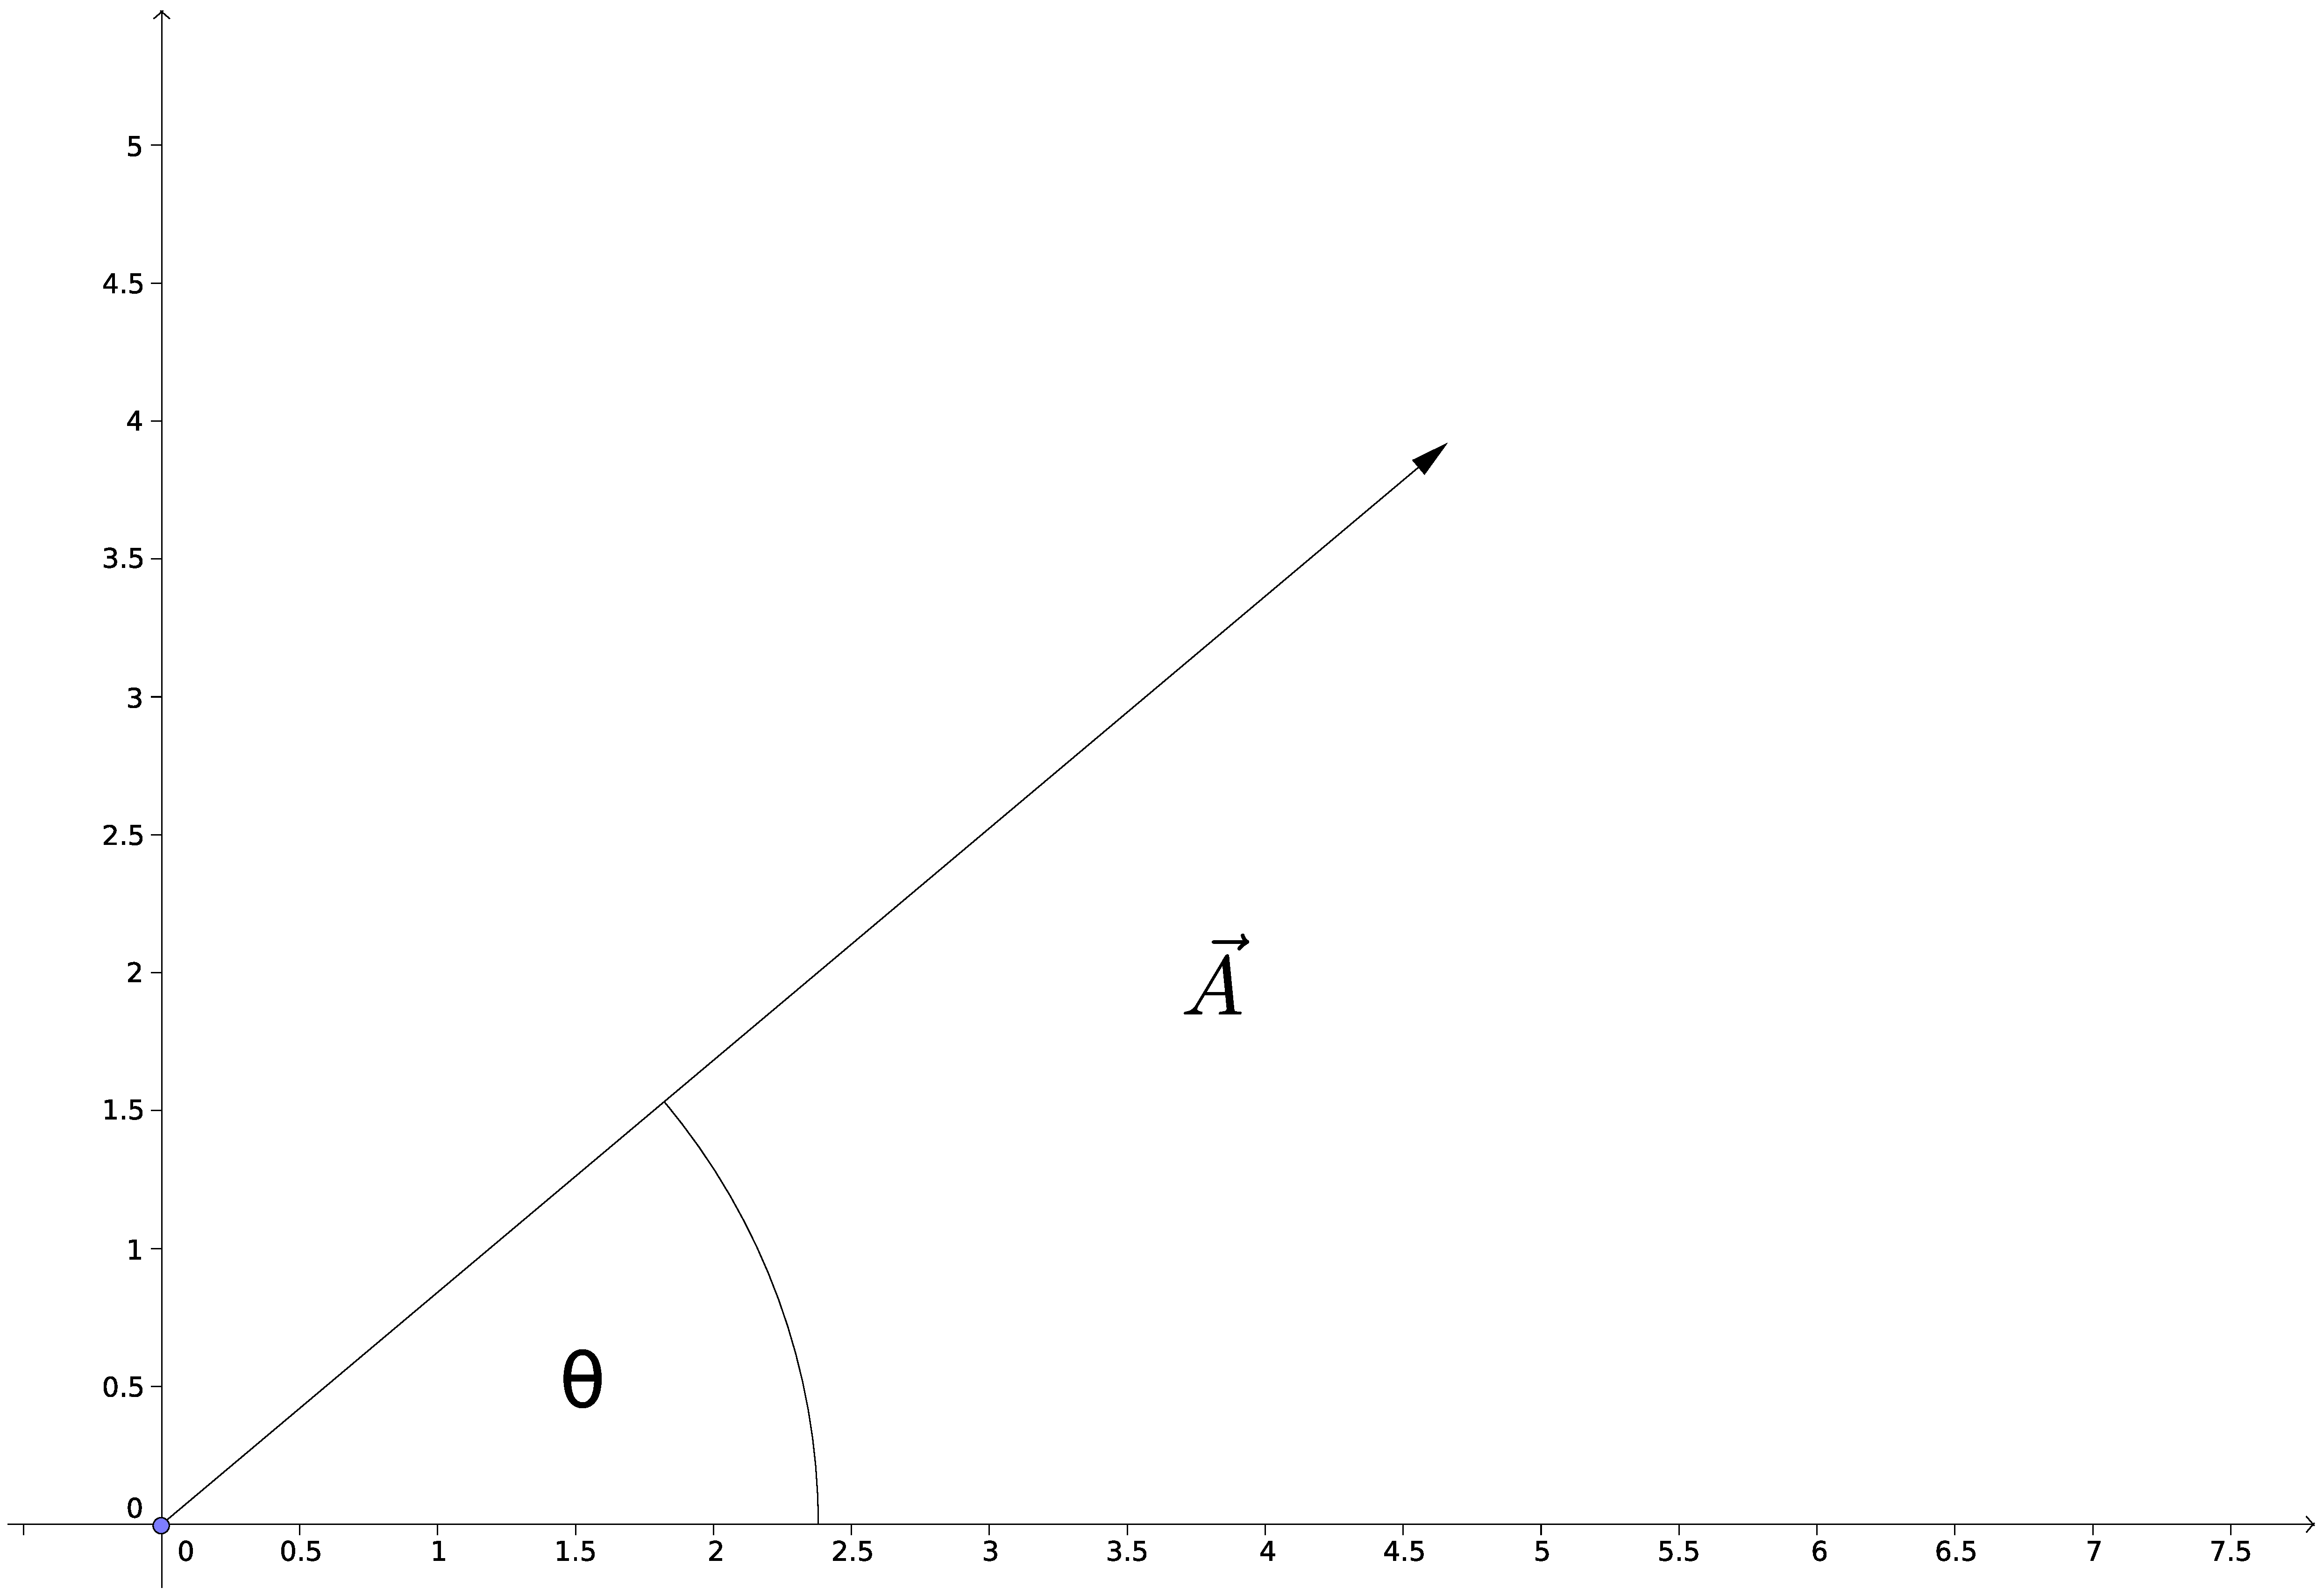
\includegraphics[width=0.7\textwidth]{images/vector_uno.eps}
  \caption{\small{Representación de un vector $\vec{A}$ en el plano cartesiano.}}
   \end{figure}

\textbf{Módulo}\\

El módulo de un vector queda definido como la longitud o tamaño que tiene la flecha que lo representa gráficamente y se 
representa como A, $|\vec{A}|$ ó $\|\vec{A}\|$. También denominado como la intensidad del vector.\\

\textbf{Dirección:}\\

Es el ángulo ($\theta$) que se forma desde la horizontal hasta el vector tomando el sentido antihorario como positivo y negativo 
en el sentido horario.\\

\textbf{Sentido:}\\

El sentido se refiere a la línea acción del vector, ó mejor dicho hacia donde apunta la flecha del vector.\\

Todo vector tiene un vector opuesto que se trata de un vector con el mismo módulo pero con su sentido contrario y se 
simboliza con un signo menos $-\vec{A}$.\\

\subsection{Representación en coordenadas cartesianas:}

\begin{figure}[H]
   \centering
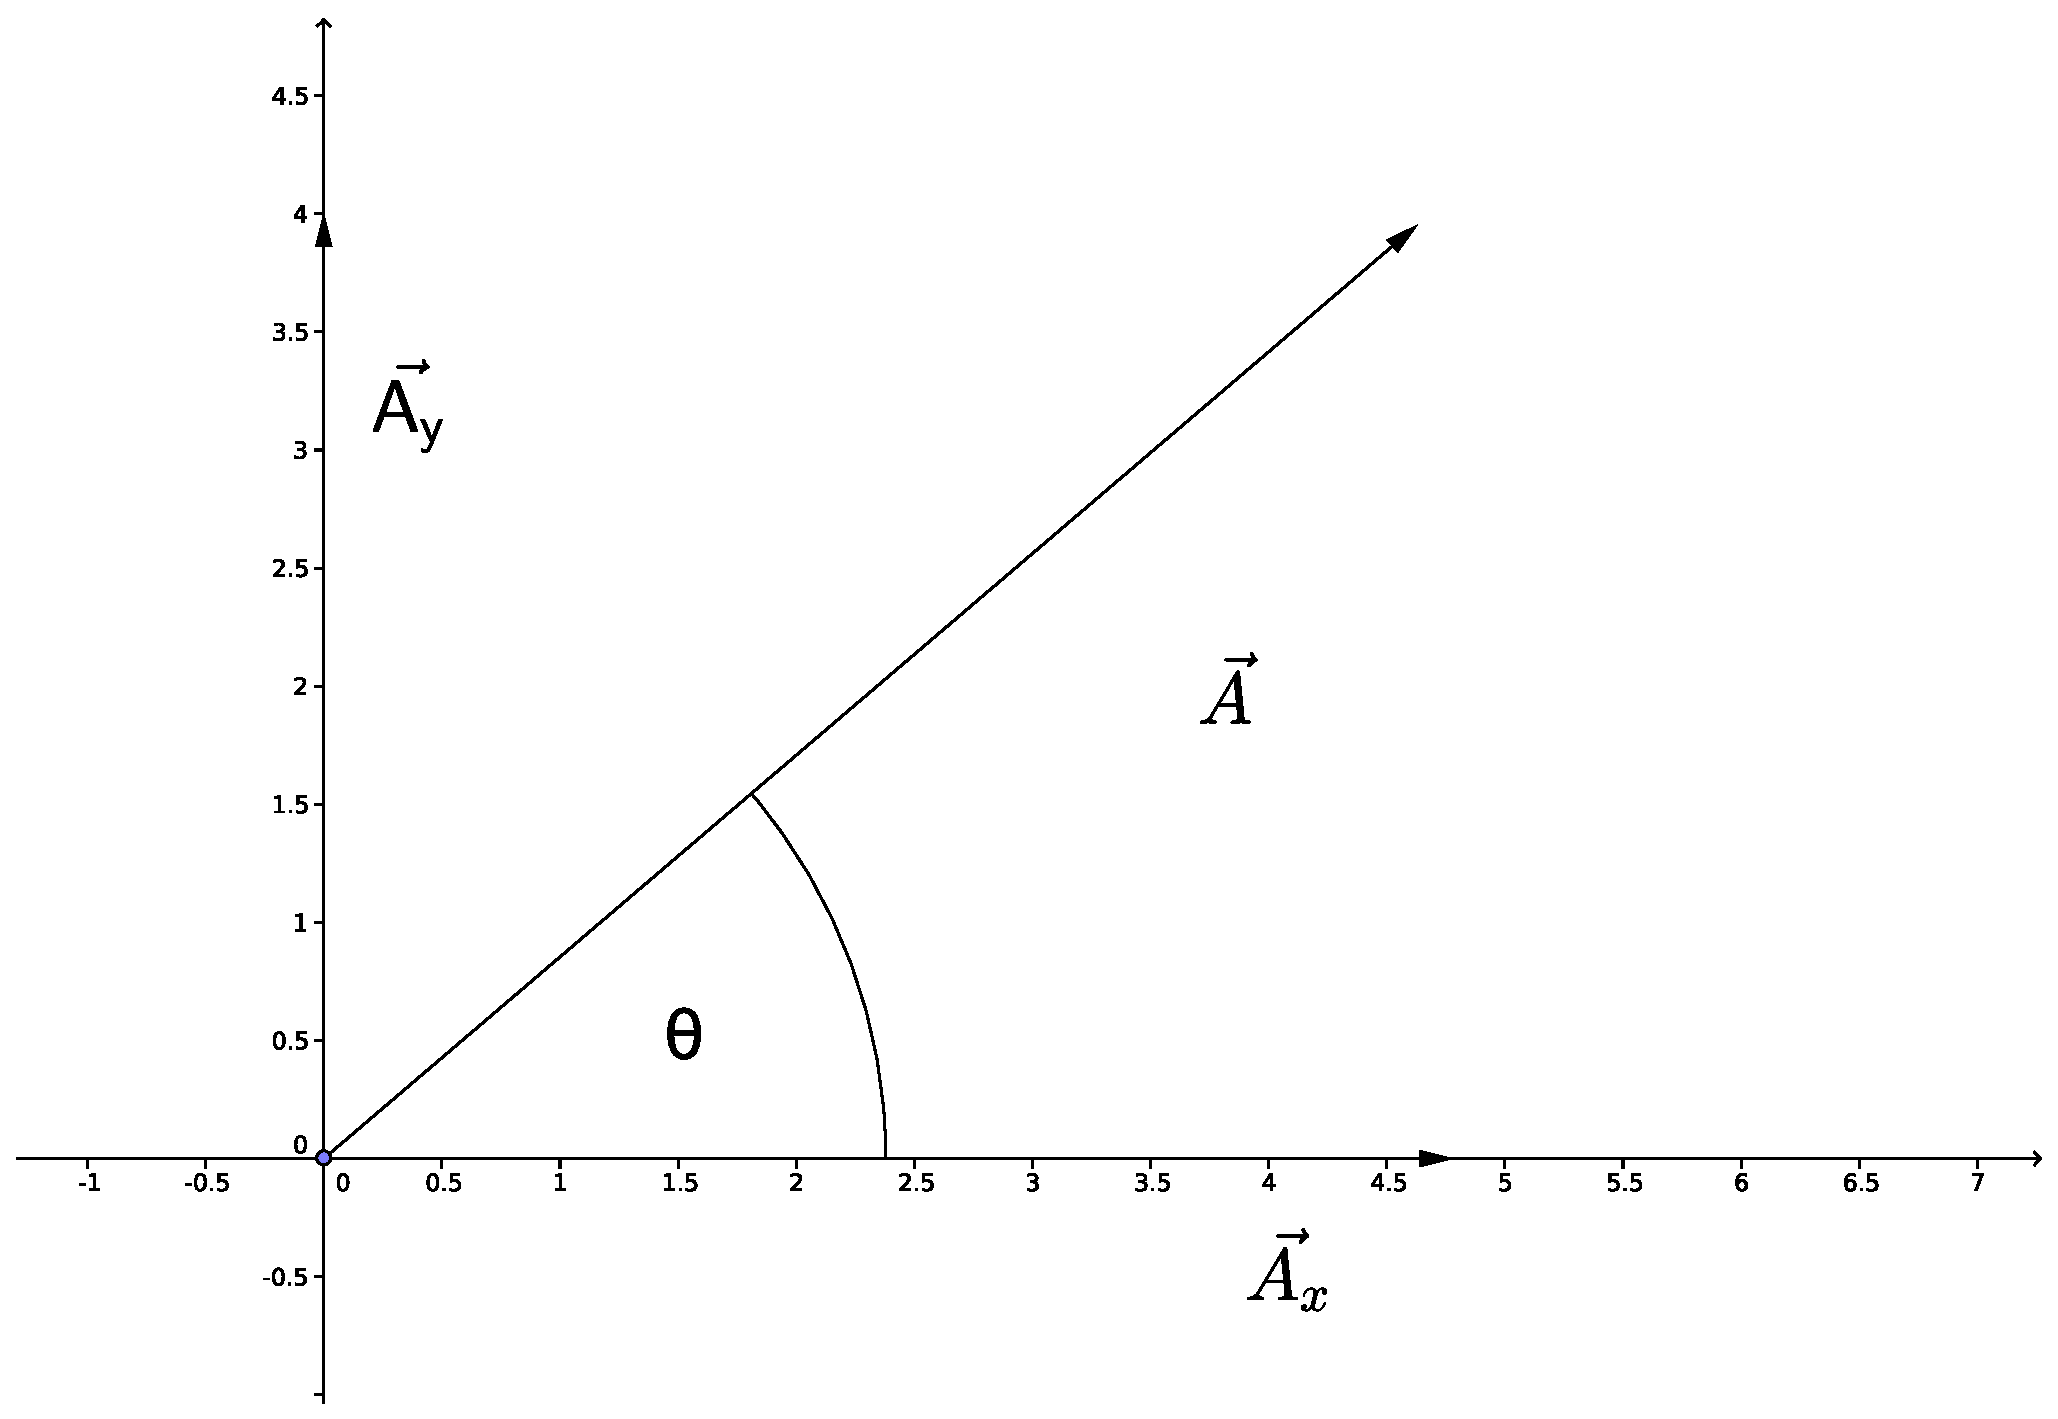
\includegraphics[width=0.7\textwidth]{images/vector_dos.eps}
  \caption{\small{Representación de las coordenadas cartesianas del vector $\vec{A}$ en el plano cartesiano.}}
   \end{figure}

En Matemáticas y Física a los vectores los representamos mediante un sistema de referencia cartesiano, y así de esta 
manera todo vector posee lo que se denomina coordenadas rectángulares. Estas componentes son las proyecciones del 
vector en cada uno de los ejes cartesianos, en otros palabras, son los vectores que se forman al proyectar 
perpendiculares desde el punto extremo del vector hacia los ejes coordenados.\\


Las coordenadas cartesianas o rectángulares de un vector $\vec{A}$, se calcula como:

\begin{equation}
A_x = Acos(\theta) \quad y \quad A_y = Asen(\theta) 
\end{equation}

donde $A_x$ es la componente del vector $\vec{A}$ en el eje de las $x$, y $A_y$ es la componente del mismo vector en el 
eje de las $y$.\\

La dirección del vector se lo encuentra de la siguiente manera:

\begin{equation}
 \theta = tan^{-1}(\frac{A_y}{A_x})
\end{equation}

, y por su puesto el módulo del vector queda definido en función de sus componentes como:

\begin{equation}
 |\vec{A}| = \sqrt{A_x^2 + A_y^2}
\end{equation}

\subsubsection{Ángulos y cosenos directores:}

Son aquello ángulos que parten desde los ejes coordenados positivos hacia el vector y cuyo valor esta en el intervalo 
de $0^\circ$ a $180^\circ$. El que parte desde el eje de las abcisas se simboliza como $\alpha$, mientras que el que 
parte desde el eje de las ordenadas se le simboliza como $\beta$.\\

Y a los cosenos directores son los cosenos de los ángulos directores simplemente:

\begin{equation}
 cos(\alpha) =\frac{A_x}{A}  \quad y \quad cos(\beta)=\frac{A_y}{A}
\end{equation}

\subsection{Representación en coordenadas polares:}

\begin{figure}[H]
   \centering
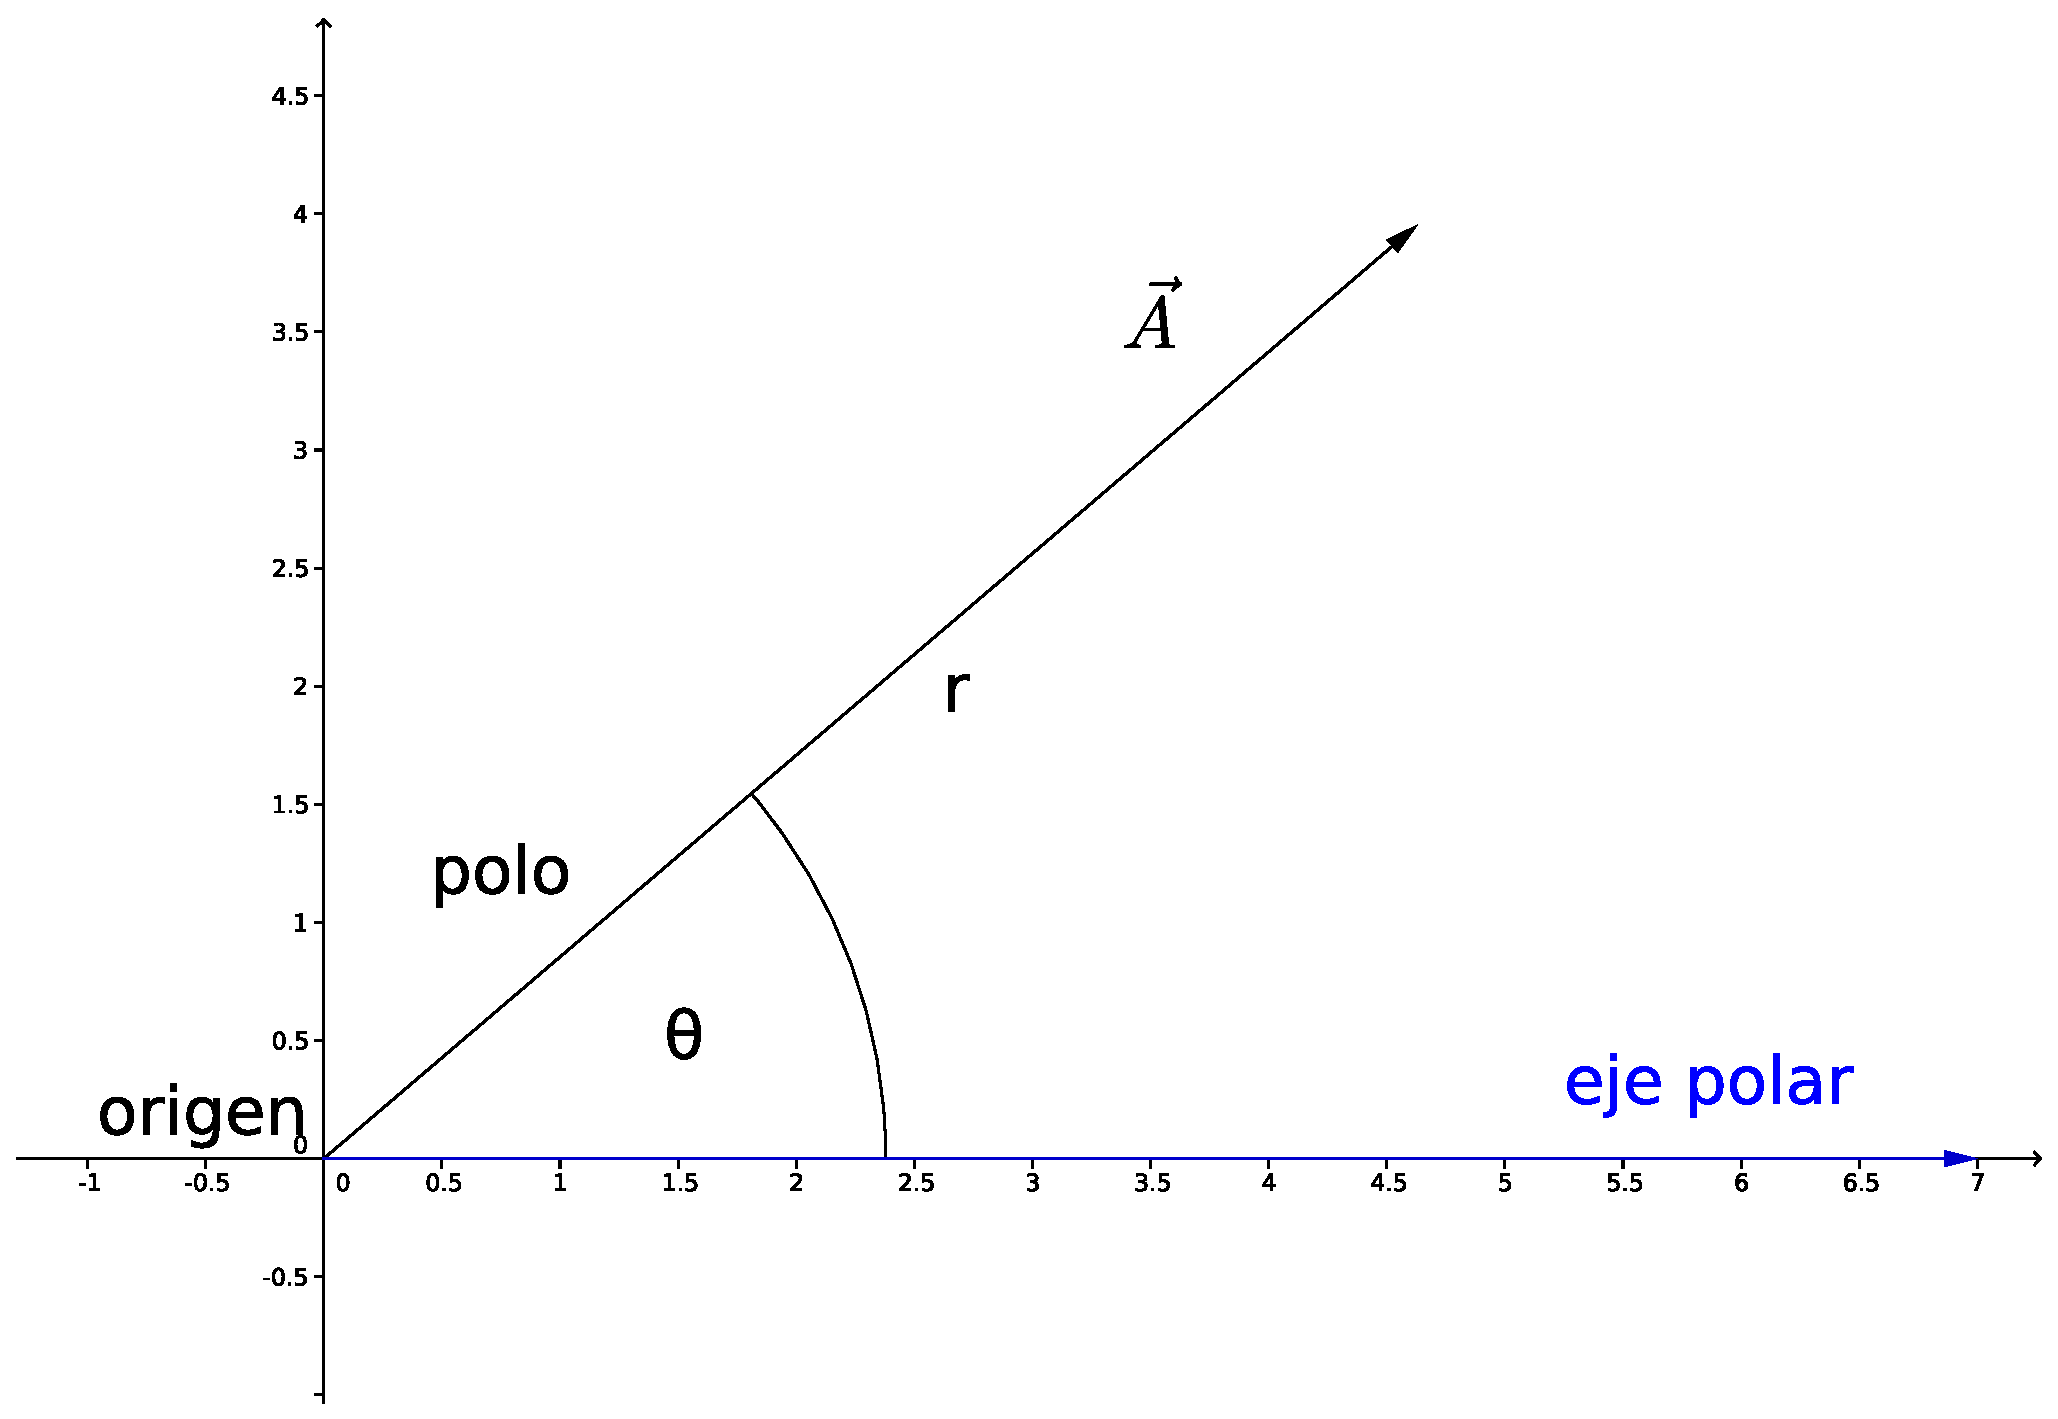
\includegraphics[width=0.7\textwidth]{images/vector_tres.eps}
  \caption{\small{Representación de las coordenadas polares del vector $\vec{A}$ en el plano cartesiano.}}
   \end{figure}

Los vectores usualmente también se los representa en función de su módulo y dirección:

\begin{equation}
 \vec{A} = (|\vec{A}|, \theta)
\end{equation}

\subsection{Representación en coordenadas geográficas:}

\begin{figure}
 \centering
 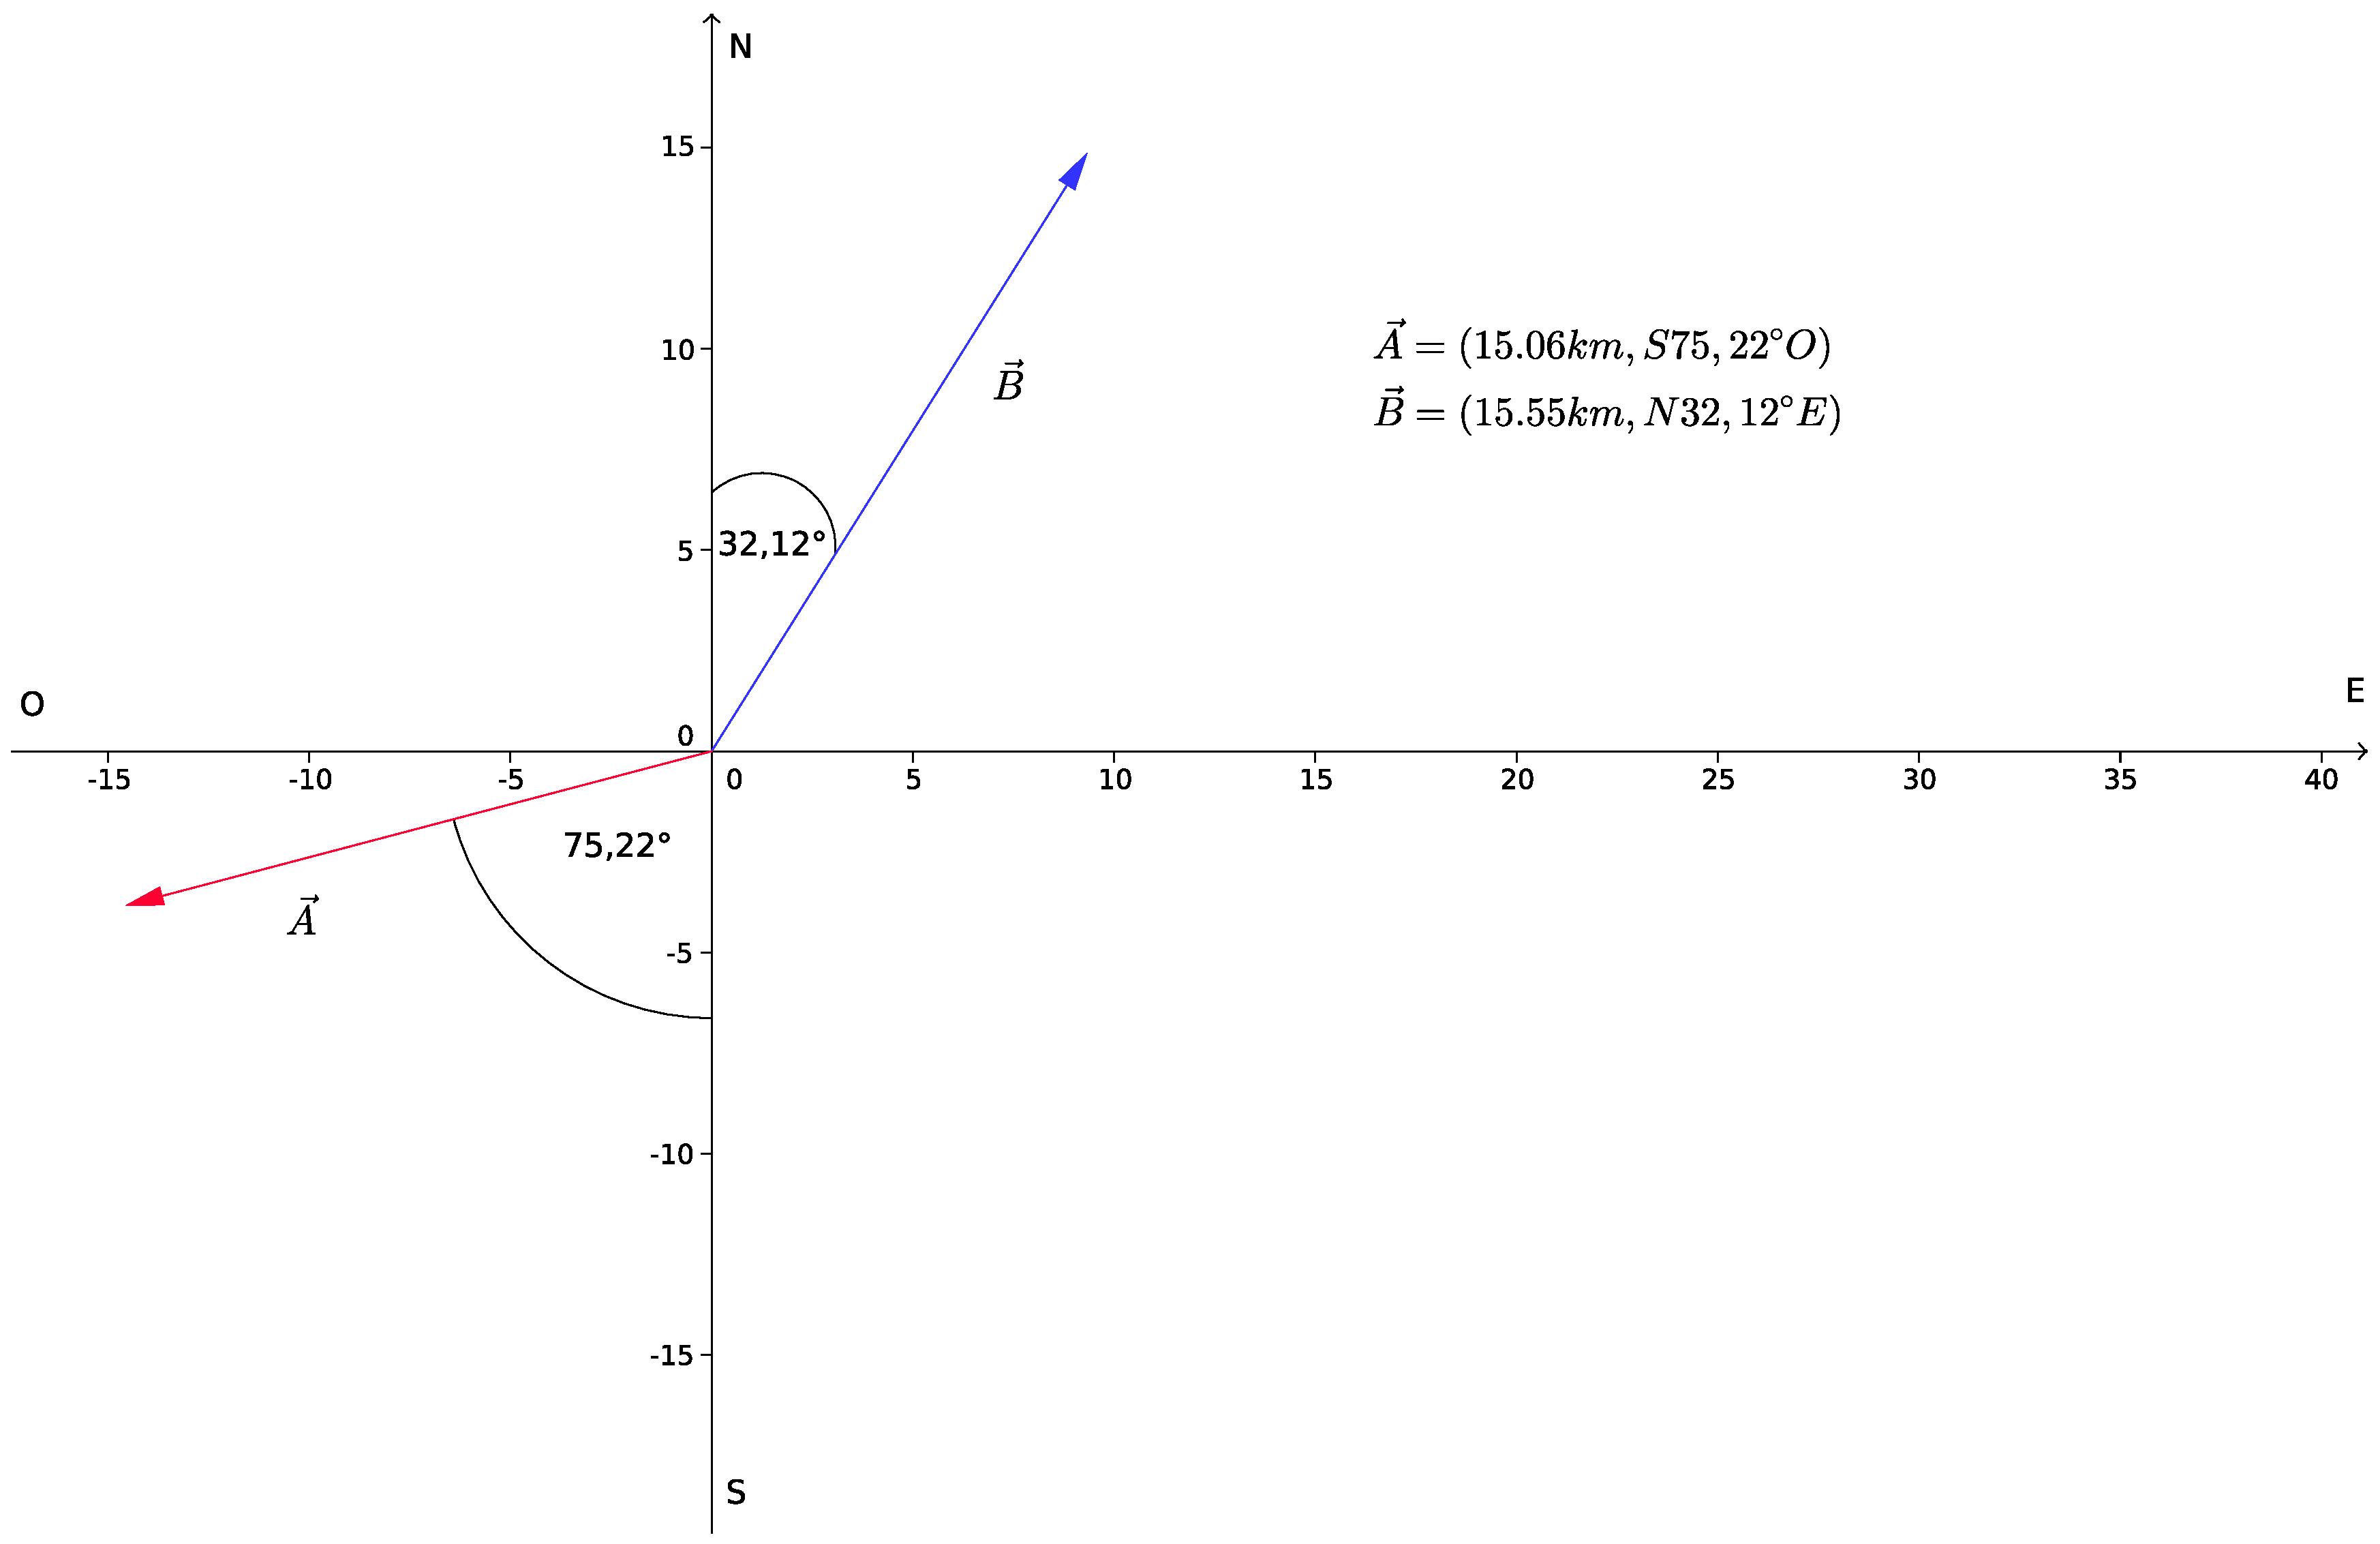
\includegraphics[width=1.1\textwidth]{images/vector_cuatro.eps}
   \caption{\small{Representación de las coordenadas geográficas de los vectores $\vec{A}$ y $B$.}}
\end{figure}

Un vector queda representado en coordenadas geográficas indicando primero su módulo, luego indicando a cual polo sea el 
Norte o el Sur al cual el vector está más cercano, posteriormente el ángulo desde ese eje hacia el vector y finalmente 
hacia que dirección sea Este o Oeste queda más cercana el vector.

\subsection{Suma y resta de vectores:}

Ya que las cantidades vectoriales poseen módulo y dirección, la suma de estas cantidades no sigue las reglas de la suma 
tradicional de los escalares.

\subsubsection{Método del paralelogramo:}

\begin{figure}
\centering
 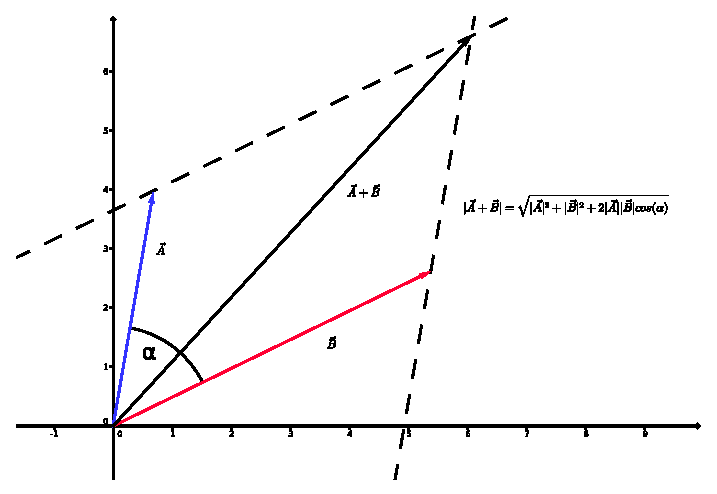
\includegraphics[scale=0.9]{images/vector_cinco.eps}
    \caption{\small{Representación de la suma entre dos vectores.}}
\end{figure}

El método del paralelogramo es un procedimiento gráfico sencillo que permite hallar la suma de dos vectores.

\begin{itemize}
 \item Primero se dibujan ambos vectores a escala, con el punto de aplicación común.
 \item Seguidamente, se completa un paralelogramo, dibujando dos segmentos paralelos a ellos.
 \item El vector suma resultante ($\vec{a} + \vec{b}$) será la diagonal del paralelogramo con origen común a los dos 
 vectores originales.
\end{itemize}

\subsubsection{Método cabeza - cola:}

\begin{figure}[H]
 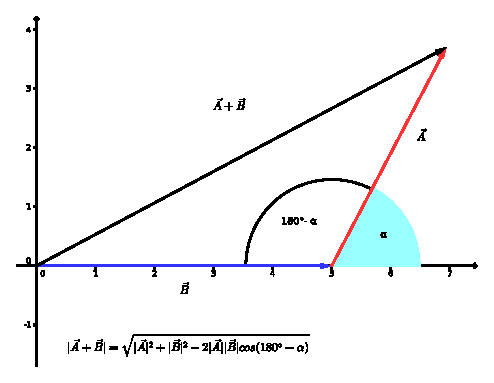
\includegraphics[scale=1.1]{images/vector_seis.eps}
    \caption{\small{Representación del método cabeza - cola.}}
 % suma-vectores-metodo-cabeza-cola.jpg: 410x261 px, 96dpi, 10.85x6.91 cm, bb=0 0 308 196
\end{figure}

Se trata de una variante del método del paralelogramo. Se desplaza el vector $\vec{b}$ paralelamente hasta el extremo 
del vector $\vec{a}$. El lado que completa el triángulo es el vector suma ($\vec{a} + \vec{b}$), cuyo inicio está en el 
extremo del primer vector $\vec{a}$ y su fin en el final del segundo vector sumando $\vec{b}$. 
    
\subsubsection{Método analítico:}     

A diferencia de los dos anteriores métodos, este se trata de un método analítico algebraico que no requiere de la 
realización del gráfico y por tanto es el más práctico y útil. Este método se trata de que primero los vectores a sumar 
deben estar expresados en sus coordenadas cartesianas y posteriormente se suman algebraicamente las componentes de los 
vectores en el eje x y así mismo en el eje y.

\begin{tcolorbox}
 Si $\vec{a} = a_x\vec{i}+a_y\vec{j}$ y $\vec{b} = b_x\vec{i}+a_y\vec{j}$, entonces el vector suma o resultante de los 
dos es: $\vec{c} =\vec{a}+\vec{b}$ tal que: $\vec{c} = (a_x + b_x)\vec{i} +(a_y+b_y)\vec{j}$. 
\end{tcolorbox}

\subsubsection{Propiedades de la suma:}

\textbf{Propiedad asociativa:}

\begin{equation}
 \vec{a} + (\vec{b} + \vec{c}) = (\vec{a} + \vec{b}) + \vec{c} = (\vec{a} + \vec{c}) +\vec{b} 
 \end{equation}

\textbf{Propiedad conmutativa:}
\begin{equation}
 \vec{a} + \vec{b} = \vec{b} + \vec{a}
\end{equation}

\textbf{Elemento opuesto:}

\begin{equation}
 \vec{a} + \vec{b} = \vec{0} \quad \text{si y solo si}\quad \vec{b} =-\vec{a} 
\end{equation}

\textbf{Elemento neutro:}

\begin{equation}
 \vec{a} + \vec{0} = \vec{a} 
\end{equation}

\subsection{Producto escalar o punto:}

\begin{figure}[H]
 \centering
 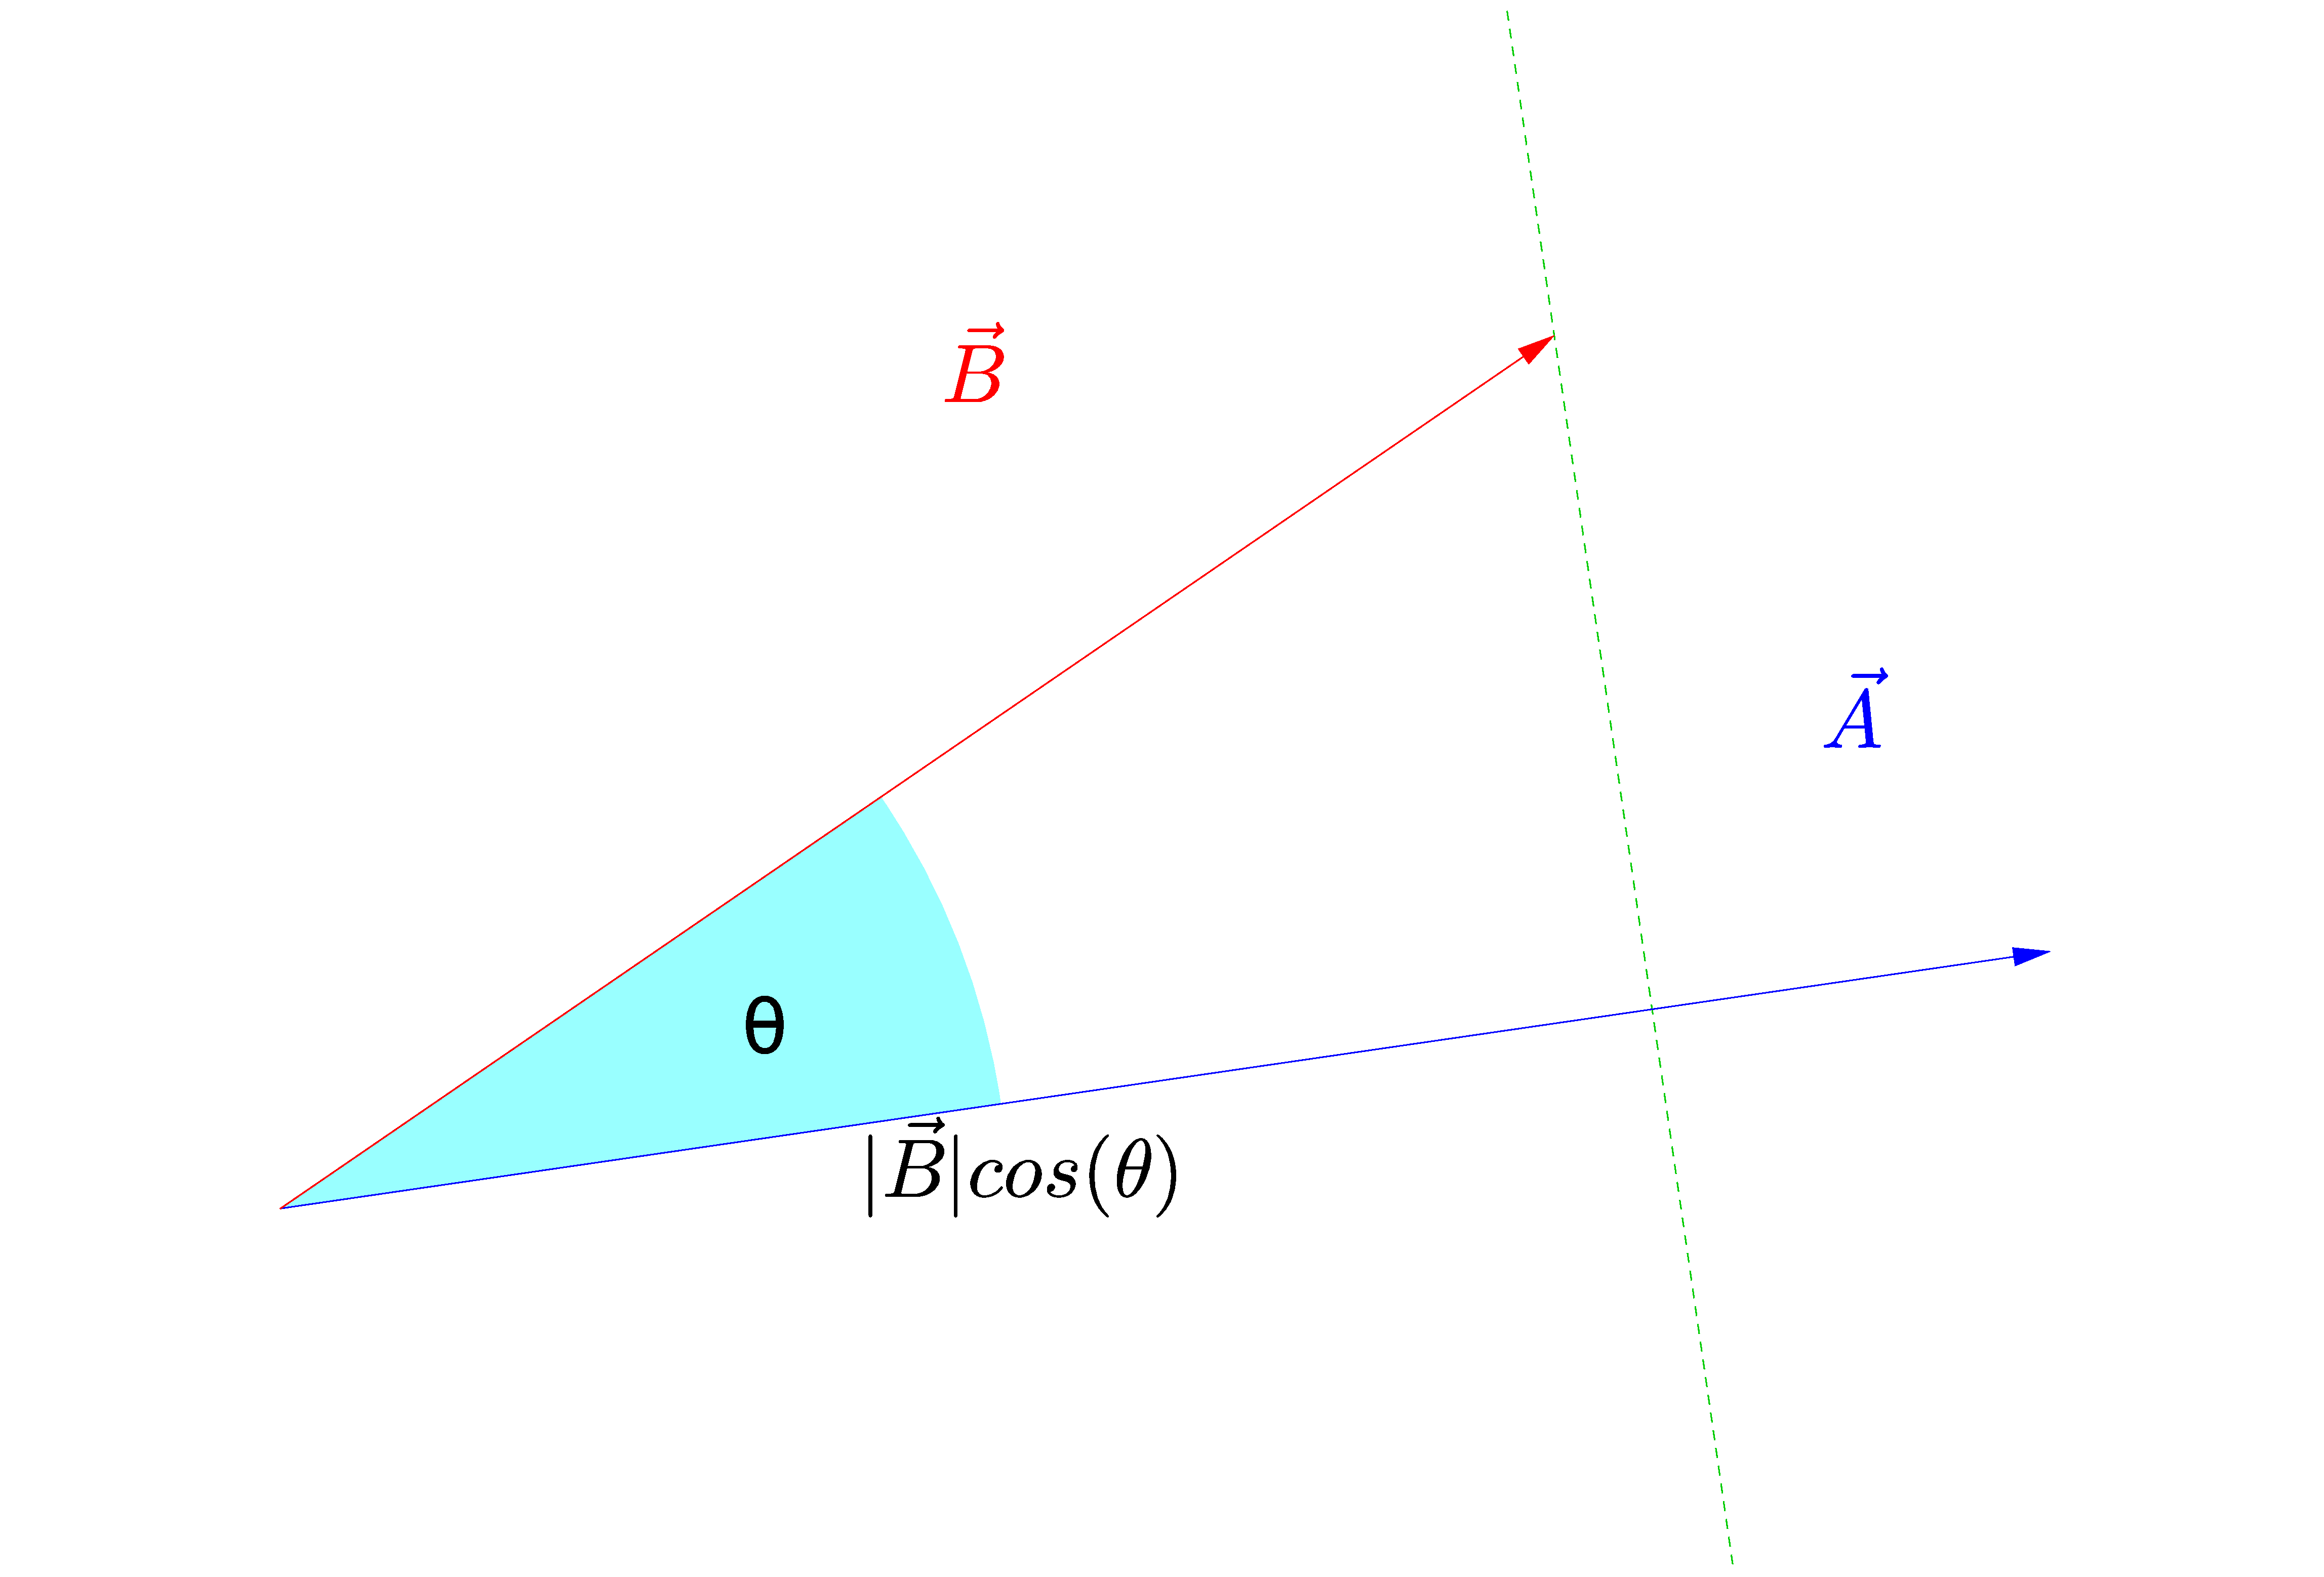
\includegraphics[width=0.7\textwidth]{images/vector_siete.eps}
 % productoescalar.png: 200x200 px, 72dpi, 7.06x7.06 cm, bb=0 0 200 200
 \caption{Ilustración geométrica del producto entre dos vectores.}
 \label{fig:escalar}
\end{figure}

Este producto se da entre dos vectores y su resultado es una cantidad escalar. Este operación se realiza de la 
siguiente manera:

\begin{tcolorbox}
Sean $\vec{a} =a_x\vec{i}+a_y\vec{j}$ y $\vec{b}=b_x\vec{i}+b_y\vec{j}$ dos vectores entonces el producto escalar 
entre ellos se define como $\vec{a}\cdot\vec{b}=|\vec{a}||\vec{b}|cos(\theta)= a_xb_x+a_yby$, donde $\theta$ es el 
ángulo formado entre los dos vectores.
\end{tcolorbox}

Así, es obvio que el producto escalar entre dos vectores que son perpendiculares es cero debido a que el ángulo entre 
ellos es de $90^\circ$.\\

Este producto tiene una interpretación geométrica que corresponde al área del paralelogramo formado entre los dos vectores.\\

A través del uso de este producto se puede calcular la proyección de un vector sobre otro de la siguiente manera:

\begin{tcolorbox}
La proyección de un vector $\vec{b}$ sobre otro vector $\vec{a}$ se define como: $\text{proj}_{\vec{a}}\vec{b} 
=|\vec{b}|cos(\theta)= \frac{\vec{a}\cdot\vec{b}}{|\vec{a}|}$.
\end{tcolorbox}

\subsection{Producto vectorial de vectores:}

\begin{figure}[H]
 \centering
 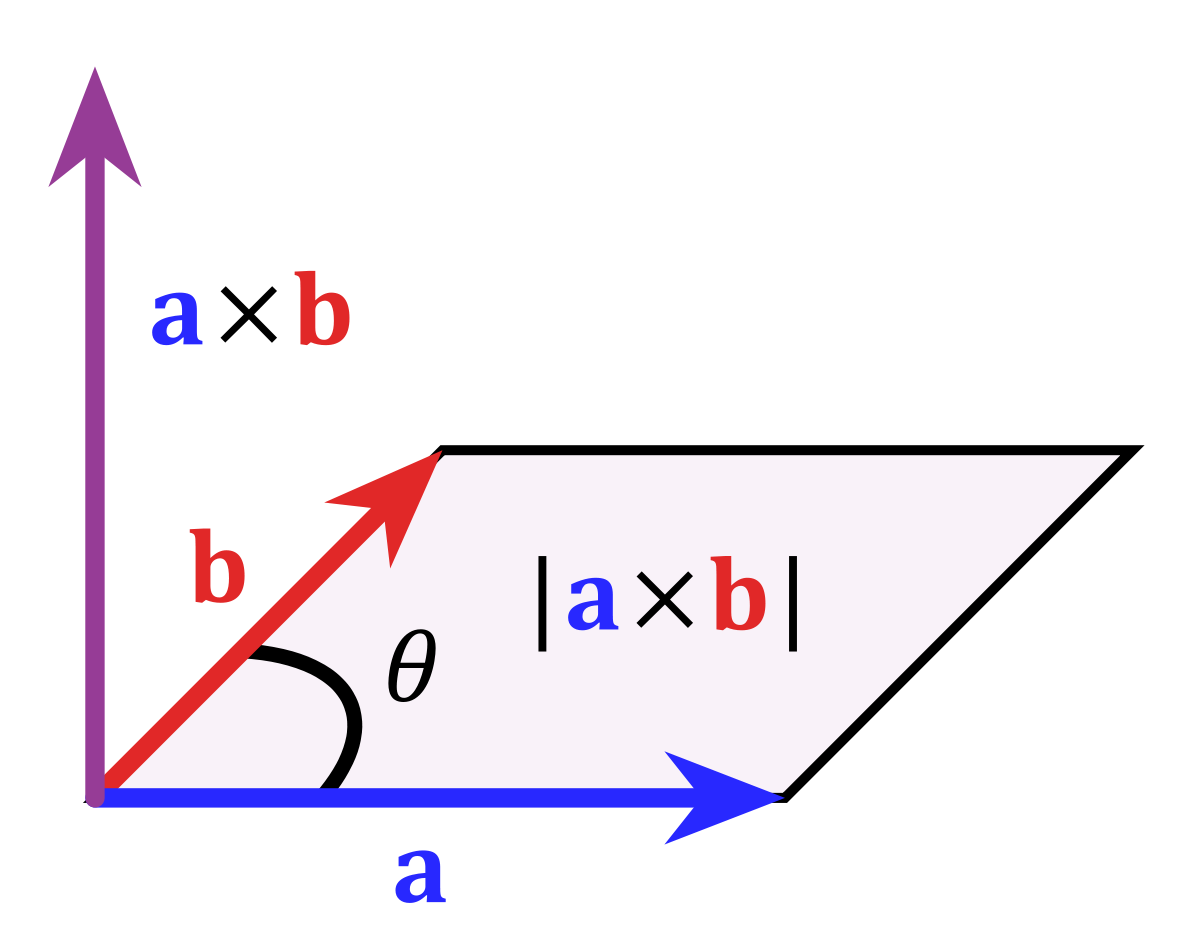
\includegraphics[scale=0.1]{images/1200px-Cross_product_parallelogram.png}
 % 1200px-Cross_product_parallelogram.svg.png: 1200x938 px, 72dpi, 42.33x33.09 cm, bb=0 0 1200 938
 \caption{Ilustración del producto vectorial entre vectores.}
 \label{fig:vectorial}
\end{figure}

Este producto se da entre dos vectores dando como resultado otro vector. Este producto se define de la siguiente manera:

\begin{tcolorbox}
 Sean $\vec{a} =a_x\vec{i}+a_y\vec{j}+a_z\vec{k}$ y $\vec{b}=b_x\vec{i}+b_y\vec{j}+b_z\vec{k}$ dos vectores entonces el 
 producto vectorial entre ellos se define como: 
\scriptsize{ 
 \[
\vec{a}\times\vec{b} =
\begin{vmatrix}
\vec{i} & \vec{j} & \vec{k} \\ 
a_x & a_y & a_z \\
b_x & b_y & b_z
\end{vmatrix} = (a_yb_z-b_ya_z)\vec{i}-(a_xb_z-a_zb_x)\vec{j}+(a_xb_y-b_xa_y)\vec{k}
\]}
\end{tcolorbox}

Siendo el vector $\vec{a}\times\vec{b}$ perpendicular a los vectores $\vec{a}$ y $\vec{b}$, y que cuyo módulo es:

\begin{equation}
 |\vec{a}\times\vec{b}|=|\vec{a}||\vec{b}|sen(\theta)
\end{equation}

Cabe resaltar que para este producto es necesario utilizar el eje coordenado espacial $z$ cuyo vector base en 
$\vec{k}$. En cuanto a la dirección del vector resultante está dada por la regla de la mano derecha. Por otro lado este 
producto da como resultado igual a cero si los vectores operandos son paralelos.

\begin{tcolorbox}
La dirección del vector $\vec{a}\times\vec{b}$ estaría definida por la dirección del pulgar, cerrando los demás dedos en torno al 
vector $\vec{a}$ primero y siguiendo con el vector $\vec{b}$.
\end{tcolorbox}

Así, cabe destacar que se cumple lo siguiente $\vec{a}\times\vec{b}=-\vec{b}\times\vec{a}$. También el módulo del producto 
vectorial de dos vectores equivale al área del paralelogramo construído en estos vectores.

\subsection{Problemas de vectores:}

\begin{enumerate}
 
 \item Calcular el vector unitario del vector $\vec{H} = 2\vec{i}+3\vec{j}$.
 
 \item Siendo el vector G = 3i – 5j, expresarlo en coordenadas polares y geográficas.
 
 \item Sean los vectores: A =(3,3), B=(-1,0) y C(2,2). Hallar la suma de esos vectores.
 
\item Sean los vectores: A =(3,3), B=(-1,0) y C(2,2). Hallar: 3A-4B+5C.

\item Que vector le debo restar al vector E =(8,7), para obtener el vector A =(2,3).
 
 \item Encuentre el módulo y dirección del vector $\vec{a}= \vec{i} - \vec{j}$.
 
 \item Encuentre el vector unitario del anterior problema.
 
 \item Hallar las coordenadas del punto C, sabiendo que B(2,2) es el punto medio de AC, A(3,1).
 
 \item Dos vectores forman entre sí un ángulo de 60°, si el valor de su resultante es de 156 unidades, y la magnitud de uno 
de los vectores componentes es de 100 unidades, ¿cuál será la magnitud del otro vector?
 
 \item Un alumno camina 50 m hacia el este, a continuación 30 m hacia el sur, después 20 m hacia el oeste, y finalmente, 10 m 
hacia el norte. Determina el vector desplazamiento desde el punto de partida hasta el punto de llegada. (incluyendo el ángulo que 
determina su dirección)
 
 \item Encuentre la suma de los vectores $\vec{c}=\vec{i}+\vec{j}$ y $\vec{d}=2\vec{i}-3\vec{d}$.
 
 \item Encuentre también la diferencia.
 
 \item Dado el vector $a =(3,-4)$, calcular el vector libre $b$ que tiene: la misma dirección y sentido que $a$ y módulo 
igual a la unidad.

\item Encuentre el producto escalar entre los siguientes vectores: $\vec{A} = 2\vec{i} + 3\vec{j}$ y $\vec{D} = 3\vec{i} - 
\vec{j}$.
 
 \item Exprese el siguiente vector en coordenadas cartesianas: c = (5, NE)
 
 \item Encuentre el vector unitario del vector que es opuesto al siguiente vector $\vec{S} =  10\vec{i}-7\vec{j}$.
 
 \item Encuentre el valor de t para el cual el siguiente vector resulta ser unitario: $\vec{v} = (t+1)\vec{i} +(t-1)\vec{j}$.

 
 \item Un vector hace un ángulo de $240^\circ$ en sentido antihorario con el eje de las abcisas y el valor de su componente 
en ese mismo eje es de 200 m, halle el vector unitario de ese vector.
 
 \item Encuentre el módulo del siguiente vector: $5\vec{d}-2\vec{c}$, donde $d=(34 m/s, 330^\circ)$ y $c = (54m/s, S20^\circ 
O)$.

\item Averigue si los vectores A = (-3,4) y B = (3,4) son perpendiculares entre si.
 
 \item Determina las coordenadas geográficas del siguiente vector: $\vec{R}=(23 m/s,N45^\circ E)$.
 
 \item Determina las coordenadas polares del siguiente vector: $\vec{T}=(7\vec{i}-4\vec{j})kgf$.
 
 \item Determina las coordenadas cartesianas del vector: $\vec{h}=(13,330^\circ)$.
 
 \item Encuentre el módulo del siguiente vector: 5d−2c, donde d = (34m/s, $330^\circ$ ) y c = (54m/s,
S$20^\circ$ O).

 \item Calcula el producto escalar entre $\vec{a}=6\vec{i}-7\vec{j}$ y $\vec{b}=-4\vec{i}+10\vec{j}$.

\item Determina si $\vec{a} = 12\vec{i}-13\vec{j}$ es perpendicular al vector $\vec{b}=4\vec{i}-3\vec{j}$.

\item Determine la proyección del vector $\vec{r} = (23 km, N40^\circ O)$ sobre el vector $\vec{q}=(40km,230^\circ)$.

\item Determine el área del paralelogramo formado por los vectores $\vec{u}=(1,1)$ y $\vec{v}=(1,-1)$.

\item Siendo los vectores $\vec{a} = (2,3)$, $\vec{b} = (-3,5)$ y $\vec{c} = (4,-1)$, calcular lo siguiente: 
$3\vec{a}\cdot\frac{1}{2}(\vec{c}+\vec{b})-7\vec{b}\cdot\vec{c}+5\vec{a}\cdot(\vec{c}-\vec{a})$ 

\item Dado los vectores $\vec{v} = 3\vec{i}-\vec{j}+4\vec{k}$ y $\vec{w}=-\vec{i}+3\vec{j}+5\vec{k}$, calcule lo 
siguiente: $\frac{1}{2}\vec{v}\times\vec{w}$.

\item Sabiendo que $\vec{A} = (m - 1) \vec{i} + (2 m + 3) \vec{j}$ y $\vec{B} = (m - 2) \vec{i} + (2 m - 19) \vec{j}$. 
Encuentre el número real m para que se cumpla que $3 \vec{A} + \vec{B} = 0$.

\item Halle el vector unitario del siguiente vector: A = (3,4), y luego encuentre su opuesto.

\item ¿Qué vector le debo restar al vector $\vec{v} = (2,4)$ para tener que el resultado sea el doble del vector $\vec{w} = 
(-2,3)$?.

\item Un automóvil recorre 3 km hacia el Norte y luego 5 km hacia el Norte $40^\circ$ Este, representar estos desplazamientos y 
hallar el desplazamiento resultante gráfica y analíticamente.

\item Calcula el valor de k sabiendo que el módulo del vector $\vec{v}$= (k, 3) es 5.

\item Dos vectores tienen como longitud 9 y 6 cm, formando entre sí ángulos de $180^\circ$, $60^\circ$, $150^\circ$, $0^\circ$. 
Halla gráficamente y analíticamente la magnitud del vector resultante y el ángulo que determina su dirección y sentido.

\item Dos vectores forman entre sí un ángulo de $60^\circ$, si el valor de su resultante es de 156 unidades, y la magnitud de uno 
de los vectores componentes es de 100 unidades, ¿cuál será la magnitud del otro vector?

\item Un alumno camina 50 m hacia el este, a continuación 30 m hacia el sur, después 20 m hacia el oeste, y finalmente, 10 m 
hacia el norte. Determina el vector desplazamiento desde el punto de partida hasta el punto de llegada. (incluyendo el ángulo que 
determina su dirección)

\item Una mosca se para en la pared de un cuarto. La esquina inferior izquierda de la pared se selecciona como el origen de un 
sistema de coordenadas cartesianas en dos dimensiones. Si la mosca está parada en el punto que tiene coordenadas (2, 1) m, (a) 
¿qué tan lejos está de la esquina del cuarto?, (b) ¿Cuál es su posición en coordenadas polares?

\end{enumerate}


\chapter{Análisis de errores en la medición}

En toda actividad técnica y científica se realizan todo tipo de mediciones de las diferentes magnitudes y estás siempre 
presentan errores, éstos son inevitables en cualquier tipo de medición. Es así, que la realización de un análisis de estos 
errores son muy necesarios para evaluar las certezas toda actividad de medición. Por ejemplo en el campo de la ingeniería una 
falla en el análisis de errores de una medición puede traer como consecuencia accidentes increíbles, por otro lado 
 en las ciencias básicas tales como la Física, el proceso de medición y el análisis de errores poseen una importancia muy 
marcada, pues están relacionados íntimamente con el método científico.\\

En el método científico se describen de una u otra forma muchos fenómenos de la naturaleza a través de modelos matemáticos 
simple o complejos, donde surge la necesidad de analizar aquellos  modelos ya sea de forma analítica, con lápiz y papel, o a 
través de simulaciones numéricas, y tratando de encontrar cuáles son sus consecuencias o predicciones. Una vez obtenido este 
análisis, se compara con experimentos y observaciones donde las mediciones están presentes. Y por tanto en este proceso lo que se 
busca hallar acuerdos entre las predicciones de los modelos y lo observado, y para ello resulta inevitable realizar un análisis 
riguroso de los errores de las mediciones para establecer concordancias coherentes y veraces, de tal modo que se obtenga como 
consecuencia conclusiones veraces y reales.

\section{El proceso de medición de errores}

En el proceso de medición siempre existe un resultado, el cual es afectado por distintos errores que surgen de la interacción 
entre el aparato de medida, el observador y el sistema bajo estudio.\\ 

Así, los errores asociados a las mediciones pueden dividirse en dos grandes clases: a) \textbf{errores sistemáticos}, y b) 
\textbf{errores aleatorios}.\\


\subsection{Errores sistemáticos:}

Los errores sistemáticos se cometen de una misma manera cada vez que se mide.  Pueden estar originados en los defectos de los 
instrumentos de medida, en una particularidad del operador o del proceso de medición, etc. Estos errores son llamados también 
errores corregibles o determinados, a fines de distinguirlos de los errores aleatorios, los cuales se encuentran en toda medición 
y están fuera del control del observador. Los errores sistemáticos no se manifiestan como fluctuaciones aleatorias en los 
resultados de las mediciones. Por lo tanto, dado que el mismo error está involucrado en cada medición, no pueden eliminarse 
simplemente repitiendo las mediciones varias veces. En consecuencia, estos errores pueden eliminarse sólo después de realizar 
cuidadosas calibraciones y análisis de todas las posibles correcciones. 

\subsection{Errores aleatorios:}

Los errores aleatorios o accidentales, aparecen como fluctuaciones al azar en los valores de mediciones consecutivas. Estas 
variaciones aleatorias se deben a pequeños errores que escapan al control del observador. Por ejemplo, 
si se observa varias veces la presión indicada por la escala de un barómetro, los valores fluctuarán alrededor de un valor medio. 
De hecho de manera estricta se puede afirmar que no se puede obtener el valor verdadero de ninguna cantidad, sino sólo una 
aproximación. El propósito del tratamiento de los datos experimentales es justamente determinar el valor más probable de una 
cantidad medida y estimar su confiabilidad.

 \section{Origen de los errores}
 
Independientemente  de  la  naturaleza  de  los  errores,  estos  pueden  deberse  a  causas  que pueden clasificarse de la 
siguiente manera:

\subsection{Errores  debidos  al  observador:} 

Son los que se atribuyen a un defecto en las percepciones sensoriales del 
observador (como por ejemplo mala visión) o a la posición incorrecta del mismo para observar la experiencia.

\subsection{Errores  debidos  al  instrumento:} 

Estos errores dependen del instrumento utilizado y pueden dividirse en: 

\begin{itemize}
 \item[a)] Defecto de construcción de escala o un corrimiento permanente de la misma: se corrigen con una correcta calibración.
 
 \item[b)] Deficiencias de construcción o desgastes: estos errores los poseen todos los instrumentos y son muy difíciles de  
detectar (se  pueden  acotar  con  un  correcto mantenimiento del aparato).
 
 \item[c)] Limitaciones propias del sistema de lectura: este tipo de error se entiende mejor con ejemplos: el grosor de la aguja 
 indicadora o el espesor de la línea de división de la escala en un instrumento analógico.
 \end{itemize}


\subsection{Errores debido al modelo físico  elegido:} 

Estos errores provienen  de  las  aproximaciones realizadas al modelar la realidad con fundamentos teóricos. Por ejemplo, para  
calcular el período de un péndulo se asume que este es puntual, el hilo es de masa despreciable y los ángulos pequeños.

\subsection{Errores causados por el propio acto de medición:} 

Estos errores se deben a que todas las veces que un experimentador hace una observación altera el fenómeno que esta estudiando. 
Por ejemplo, cuando se mide la presión de un neumático con un manómetro, se libera algo de aire alterando la presión a medir.  

\subsection{Errores producidos por condiciones externas al proceso de medición:}  

Este tipo de  errores  se deben a las condiciones ambientales en las cuales se realiza una experiencia.  Son, en general, 
calculables en forma de correcciones para cada instrumento y para cada método de medida.  


\section{Precisión y exactitud}

Es costumbre generalizada, sobre todo en algunas normas relativas a instrumentos de medida, designar a la exactitud como la 
precisión de los mismos pero, tienen significados muy diferentes. \textbf{La exactitud} da una idea del grado de aproximación con 
que el valor medido concuerda con el valor  verdadero;  es decir, es la cercanía del valor experimental obtenido respecto al 
valor real de dicha medida. Por otro lado, \textbf{La precisión} se refiere a la repetibilidad de los resultados; es decir, el  
grado con el cual las medidas sucesivas arrojan idénticos valores. También está asociada a la sensibilidad o menor variación 
de la magnitud que se pueda detectar con un instrumento (o un método de medición).\\

Existen dos maneras de cuantificar el error de medición:\\

Mediante el llamado \textbf{error absoluto}, que corresponde a la diferencia entre el valor medido $X_m$ y el valor real $X_r$:

\begin{equation}
 E_{abs} = |X_m - X_r |
\end{equation}

Ó mediante  el  llamado \textbf{error  relativo},  que  corresponde  a  el  cociente  entre  el  error  absoluto  y  el valor 
real.

\begin{equation}
 E_{rel} =  E/X_r
 \end{equation}

\subsection{Resultado de una medición:}

El resultado de cualquier proceso de medición se compone del valor medido, de un símbolo que representa la unidad y del error que 
indica la ``exactitud'' con que se conoce el valor medido.  Con lo cual, el resultado de una medición queda expresado de la 
siguiente forma:

\begin{equation}
 X = (X_m \pm E_{abs})[\text{unidad de medida}]
\end{equation}

donde $X$ es la  magnitud que se desea medir o conocer; $X_m$  es  el  valor  medido  (representa  el número de veces que 
contiene a la unidad seleccionada); $E_{abs}$ es el error absoluto o incerteza (indica la exactitud con que se conoce el valor 
medido). Entonces, por medirse se entiende conocer el valor de una magnitud y conocer también el error con que se la mide en la 
unidad seleccionada.

\subsection{Intervalo de incerteza:}

Se dice que hay concordancia entre las predicciones teóricas de una hipótesis, modelo o teoría y los resultados de una medición,  
cuando  ambos  valores  coinciden  dentro  de  un  rango  definido  por  el error de medición. El error ``E'' define alrededor 
del valor medido un intervalo de incerteza igual al doble  del  error  (2E). Es otras palabras, indica una zona (intervalo) 
dentro de la cual está comprendido el verdadero valor de la magnitud: $(x_m - E, X_m + E)$.

\section{Cifras Significativas (c.s.)}

Los científicos e ingenieros procuran que sus datos experimentales no digan más de lo que pueden decir  (``asegurar'')  según  
las condiciones de medida en que fueron obtenidos. Por ello, ponen cuidado en el número de cifras con que expresan el resultado  
de una medición. El  propósito  de ello  es  incluir sólo aquellas  que  tienen  algún  significado  experimental. Tales cifras  
reciben  el nombre de cifras significativas.  Una cifra es significativa cuando se la conoce con una exactitud aceptable. Así,  
cuando  se  mide  con  un  termómetro  que  aprecia  hasta  $0,1^\circ C$  no  tiene  ningún sentido que se escriban resultados, 
por ejemplo, del tipo $36,25^\circ C$ o $22,175^\circ C$.\\

Esto es, la cantidad de  decimales  después  de  la  coma  esta  
relacionada  con  la  exactitud  del  instrumento  (y  no  con  la cantidad de dígitos que maneja una calculadora). Las cifras 
significativas no tienen ninguna relación \textit{fija} con la posición de la coma decimal; esto es, no tiene siempre que ser 1 o 
2 lugares.  La cantidad de decimales depende del instrumento utilizado para medir.\\


Una posible fuente de ambigüedad se presenta con el número de cifras significativas cuando se hace  un  cambio  de  unidades. El  
número  de  cifras  significativas  de  un  resultado  es  el  mismo, cualquiera que sea la unidad en la que se lo exprese. Dada 
una cantidad, la pregunta es ¿cuáles son cifras significativas?: a)Los  ceros  a  la  izquierda no  son  c.s.: Cuando  los  ceros  
figuran  como  primeras  cifras  de  un resultado  no  son  considerados  como  cifras  significativas. No  indican  exactitud  en 
 el resultado de la medición sino que indican el orden de magnitud de la unidad que acompaña al mismo, y b) Los  ceros  a  la  
derecha: Cuando  los  ceros  figuran  como  últimas  cifras  de  números  enteros, ello no implica que deban ser considerados 
necesariamente como cifras significativas.

\subsection{Empleo de cifras significativas:}


\subsubsection{Cifras significativas en operaciones aritméticas:}

Cuando se dispone de una calculadora electrónica parece como si fuese ``correcto'' o ``más exacto'' escribir los resultados con 
tantas cifras decimales como aparecen en pantalla, pero esto la mayoría de las veces carece de sentido. Para expresar 
correctamente los resultados de operaciones aritméticas, mediante cifras significativas, es necesario tener en cuenta que dicho 
resultado no puede tener más decimales que el número de menor cantidad de decimales involucrado en la operación.

\subsubsection{Reglas de aproximación o acotación de números:} 

Cuando  se  requiere  acotar  la  parte  decimal  de  un  número  hay  que  fijarse  en  el  número  de  su derecha. Si  éste  es 
 mayor o igual que  5,  entonces  se  redondea  incrementando  el  “último”  dígito significativo en +1.  Si es menor a 5, el 
``último'' dígito significativo permanece sin cambio; es decir, no se modifica. (éste método no es general pero es el que 
utilizaremos en este libro)

\section{Teoría Estadística de errores:}


En este apartado analizaremos los errores en la medición de una magnitud que se repite N veces.  Dado el carácter al azar de los 
errores es claro que, al promediar  los  resultados,  el  promedio  estará  menos  afectado  por  las  desviaciones estadísticas 
 que los valores individuales.  Se asume que no se cometen errores groseros y que los sistemáticos han sido debidamente acotados 
de manera tal que, los únicos errores a considerar sean los casuales. Para  analizar  la  serie  de N  mediciones  de  una  misma 
 magnitud  obtenida  en  igualdad  de condiciones  se  emplea  la  \textbf{Teoría  Estadística}.\\
 
La teoría estadística se basa en los tres postulados de Gauss:\\

i) Dada una serie de mediciones $x_1$, $x_2$,$\ldots$, $x_N$, la 
mejor estimación de la magnitud medida o valor más probable de la misma es el promedio aritmético de todas las mediciones de esa 
cantidad efectuadas en las mismas condiciones:

\begin{equation}
 \overline{x} = \frac{\sum_{i = 1}^{N} x_i}{N} = \frac{x_1+x_2+\ldots + x_N}{N}
\end{equation}

ii) Es igualmente probable cometer errores del mismo valor numérico y distinto signo.\\

iii) En  una  serie  de  mediciones, es tanto más probable un error cuanto menor sea su valorabsoluto. Es decir, los errores más 
pequeños son los más probables de cometer.\\

Se dice que la calidad de una medición será tanto mejor cuanto más parecidos sean entre sí los valores medidos, o dicho de otra 
forma, más parecidos al valor medio $\overline{x}$. Otros conceptos útiles en el análisis de una serie de mediciones son la 
mediana y la moda. La mediana hace énfasis en el verdadero ``centro'' del conjunto de datos. En otras palabras, la mediana es el 
valor central de un conjunto de mediciones ordenado por magnitud creciente o decreciente.  El  propósito  de  la  misma  es  
reflejar  la  tendencia  central  de  la  serie  de  medidas  de  manera  que  no esté  influenciada  por  los  valores  
extremos. Mientras  que  la moda (M)  es  aquel  valor  que  ocurre más  a  menudo  o  con  mayor  frecuencia. La moda puede 
no existir, y cuando existe no necesariamente es única.
 
\subsection{Error estadístico de la serie de N medidas:}

Dada  una  serie  de N  mediciones  de  la  magnitud $x$,  se  define  en  primer  lugar la desviación  de  la medición $epsilon_i$,  
la  cual  se  mide  respecto  del  valor  medio $x$  y  no  es  más  que  la  diferencia  existente entre  el  valor i-ésimo  
medido y el  valor  más  probable  (o  valor  medio  o  promedio  aritmético  de  la serie, i.e. $\overline{x}$): 

\begin{equation}
\epsilon_{i} = x - x_{i} = f_{i}( x - x_{i} ) 
\end{equation}

siendo, de nuevo, $f_i$ las veces que el i-ésimo valor $x_i$ se repite. La  sumatoria  de  la  desviación  ($\sum_i \epsilon_i$)  
no  tiene  significado  físico  e  incluso  puede  ser  cero;  en cambio, sí lo tiene la sumatoria de las desviaciones al 
cuadrado ($\sum_i \epsilon_i^2$) que representa la forma en que los valores individuales fluctúan alrededor del promedio.  Pero 
esta última cantidad depende de N.  Para independizarse de N es que se define la \textbf{varianza} $\nu$ como el promedio de las 
desviaciones cuadráticas:

\begin{equation}
 \nu = \frac{\sum_i \epsilon_i^2}{N}
\end{equation}

Es más común utilizar la raíz cuadrada de la varianza ($\sqrt{\nu}$) que proporciona la distribución de las mediciones alrededor 
del valor más probable ($\overline{x}$) pero con la misma unidad que los datos originales.  Dicha  cantidad  se  denomina  la 
dispersión  ó desviación  estándar  ó error  cuadrático  medio ($\sigma$)  de cada medida:

\begin{equation}
 \sigma = \sqrt{\nu} =\sqrt{\frac{\sum_i \epsilon_i^2}{N}}
\end{equation}

La desviación estándar es una medida del grado de dispersión de los datos alrededor del valor promedio.  Dicho de otra manera, la 
desviación estándar es simplemente el ``promedio'' o variación esperada con respecto de la media aritmética.  Una desviación 
estándar grande indica que los puntos están lejos de la media, y una desviación pequeña indica que los datos están agrupados 
cercanos a la media.\\

Un parámetro que nos  da  el  orden  de  magnitud  con  el  cuál  el  promedio  habrá  de  fluctuar  alrededor  del 
``verdadero  valor''  de  la  magnitud  en  cuestión  y  se  mantendrá  casi  constante  cuando  el  número  de observaciones es 
suficientemente grande (N grande) es el error estadístico:

\begin{equation}
 E_{est}=\frac{\sigma}{\sqrt{N}}
\end{equation}

, cuanto más mediciones se realicen, tanto más se acercará el promedio al ``verdadero valor'' de la magnitud en cuestión, y la 
fluctuación será cada vez menor.  Es  por  ello  que  el  promedio  es  utilizado  como  ente  representativo  del  valor  más  
probable  de  una magnitud.  

Hay que tomar en cuenta lo siguiente para nuestros procesos de medición:\\

\textit{Como no tiene sentido disminuir $E_{est}$ más allá de la apreciación $\Delta x$ del instrumento de medición, resulta más  
correcto cambiar el instrumento o mejorar el método que aumentar el número de mediciones. Es preferible obtener veinte ``buenas'' 
medidas y no mil mediocres.}\\

\subsection{Error medio cuadrático (rms)}

En Física experimental resulta muchas veces evaluar el error cuadrática metido para una colección de N valores 
{$x_1, x_2, \ldots , x_N$} de una variable discreta $x$, el cual dado por:


\begin{equation}
 x_{rms} =\sqrt{  \frac{1}{N}\sum_{i = 1}^N x_{i}^2 }
\end{equation}

\vspace{1.5cm}

Con todo lo anterior analizado es posible dar como medida final de las $x_i$ mediciones como:

\begin{equation}
 x =  \overline{x} \pm \sigma
\end{equation}









 
 


\chapter{Física}

\textit{``Sería muy triste ser un átomo en el universo sin los físicos. Y los físicos están hechos de átomos. Un físico es la 
forma de un átomo de saber que hay átomos.''} \textbf{George Wald}
\vspace{1.0 cm}

\section{Física: Filosofía Natural}

La Física es parte de las Ciencias Naturales, ésta ciencia estudia a la energía, la materia, el tiempo y el espacio en toda su 
comportamiento, estructura, e interacciones. El término \textbf{Física} proviene del lat. physica, y este del griego 
$\varphi\upsilon\sigma\iota\kappa o\varsigma$, 'natural, relativo a la naturaleza'.\\

Una muy precisa definición de Física es la siguiente:

\begin{tcolorbox}
Ciencia que estudia las leyes fundamentales que rigen el Universo.
\end{tcolorbox}

Entiendiéndose como Universo el conjunto de cuerpos celestes y materia interestellar que se encuentra en el espacio. También otra 
precisa definición es la siguiente:

\begin{tcolorbox}
Ciencia natural que estudia los fenómenos físicos y lo que ocurre en la naturaleza, los componentes fundamentales del Universo, 
la 
energía, la materia, el espacio-tiempo y las interacciones fundamentales. La Física es una ciencia básica estrechamente vinculada 
con las matemáticas y la lógica en la formulación y cuantificación de sus principios.
\end{tcolorbox}

En esta ciencia se estudia aquellos fenómenos llamados físicos en los cuales la estructura química de las materia permanence 
inalterada. Ejemplos de fenómenos físicos: la ebullición del agua, la caída de los cuerpos, la transmición del calor, la 
evaporización de los líquidos, etc.\\

Esta disciplina incentiva competencias, métodos y una cultura científica que permiten comprender nuestro mundo físico y viviente, 
para luego actuar sobre él. Sus procesos cognitivos se han convertido en protagonistas del saber y hacer científico y tecnológico 
general, ayudando a conocer, teorizar, experimentar y evaluar actos dentro de diversos sistemas, clarificando causa y efecto en 
numerosos fenómenos. De esta manera, la física contribuye a la conservación y preservación de recursos, facilitando la toma de 
conciencia y la participación efectiva y sostenida de la sociedad en la resolución de sus propios problemas.\\

Y como podemos apreciar nos encontramos viviendo en un mundo tecnológico y científico, siendo la física parte fundamental del 
mundo, ya que esta abarca desde lo infinitamente pequeño, como es el caso de la física de las partículas, a lo infinitamente 
grande, como es el caso de la astrofísica. Es por eso que no debe ser extraño para nosotros que la física se encuentre presente 
en 
cada ámbito del progreso técnico y científico.\\

La Física trata de responder dos grandes preguntas: ¿Cómo funciona el Universo? y ¿Por qué funciona?. La respuesta o las 
respuesta 
a la primera pregunta se manifiesta mediante el surgimiento de las leyes físicas, que cuyo sueño científico es lograr llegar a 
una 
sóla ley de unificación, mientras que la segunda pregunta se ve responde mediante el reconocimiento de principios físicos que a 
su 
vez responde a la inevitabilidad de los fenómenos en el Universo.


\chapter{Cinemática}

\textit{``Si en un instante determinado conociésemos la situación y la velocidad exactas de todas las partículas del universo, 
podríamos deducir por cálculos todo lo pasado y lo futuro de él.''}  \textbf{Laplace}

\section{El movimiento}

\begin{figure}[ht]
 \centering
 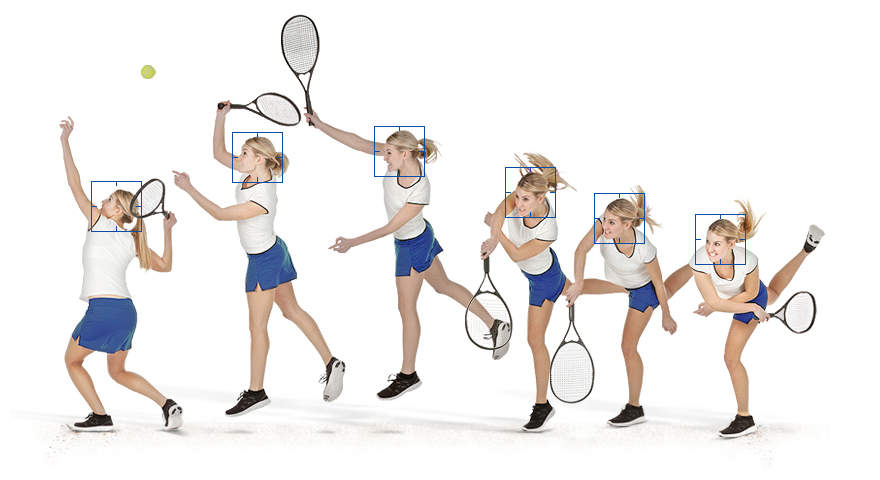
\includegraphics[scale=0.3]{images/movimiento.jpg}
 \caption{Ilustración del movimiento de una tenista.}
 \label{fig:vectorial}
\end{figure}

El estudio de la Física comienza con el fenómeno más fundamental que existe en el Universo el cual es el movimiento. Cada 
componente del Universo está en movimiento, incluso en a temperaturas muy bajas cercanas al cero absoluto el movimiento no cesa, 
y 
es por eso que el movimiento es el fenómeno más fundamental del Universo y el primer apartado a estudiar en Física.\\

La Cinemática es la rama de la Física que estudia a el movimiento sin analizar sus causas, es decir, estudia las magnitudes que 
describen la geometría del movimiento de los cuerpo.\\ 

\begin{figure}[ht]
 \centering
 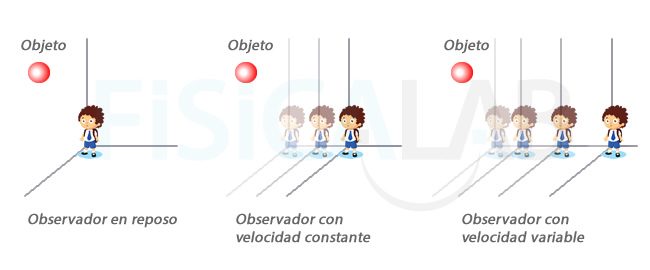
\includegraphics[scale=0.37]{images/sistema_inercial_no_inercial.jpg}
 % sistema_inercial_no_inercial.jpg: 650x270 px, 72dpi, 22.93x9.52 cm, bb=0 0 650 270
 \caption{Ilustración de tres sistemas de referencia diferentes.}
\end{figure}

Para estudiar el fenómeno del movimiento se hace referencia a uno o más observadores que analizan el movimiento y realizan las 
medidas de las magnitudes involucradas en el fenómeno, por ello es necesario plantear un sistema de referencia desde el cual el 
observador u observadores hacen sus medidas, en general el sistema de referencia es el plano cartesiano.\\

Una vez ya ubicado el sistema de referencia lo más natural es observar que el cuerpo o partícula en movimiento tendrá diferentes 
posiciones cuando el tiempo avanza, es por tanto la necesidad de definir lo que se llama vector posición.\\ 

\textbf{Vector posición:} Es el vector que indica la posición del cuerpo respecto a un sistema de referencia. Este vector tiene 
su origen en el origen del sistema de referencia (donde se supone que está un observador) y su extremo donde está el cuerpo o 
partícula de estudio.

\begin{figure}[ht]
 \centering
 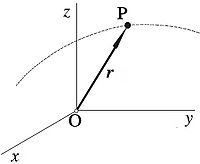
\includegraphics[scale=0.6]{images/posicion.jpg}
 % vector_de_posición.jpg: 200x164 px, 96dpi, 5.29x4.34 cm, bb=0 0 150 123
 \caption{Ilustración del vector posición.}
\end{figure}

Así, si tenemos dos posiciones diferentes del cuerpo o partícula en movimiento se puede definir lo que se llama desplazamiento.\\

\textbf{Desplazamiento:}\\

Se entiende por desplazamiento el vector o segmento recto orientado que une la posición inicial con otra posición posterior en el 
tiempo del cuerpo en movimiento; así, el origen del vector posición es la posición inicial del cuerpo y el extremo del vector 
desplazamiento se halla en la posición final del cuerpo tomada en cuenta. El vector desplazamiento ($\Delta \vec{r}$) resulta de 
hecho la resta del vector posición final ($\vec{r_f}$) con la posición inicial ($\vec{r_o}$).

\begin{equation}
 \Delta \vec{r} = \vec{r_f}-\vec{r_o}
\end{equation}

\begin{figure}[ht]
 \centering
 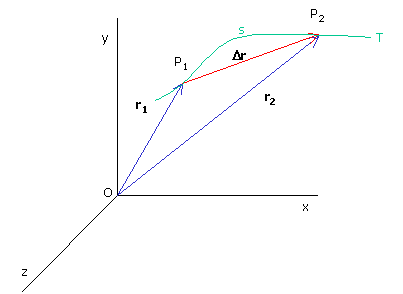
\includegraphics[scale=0.5]{images/cinematica.png}
 % cinematica.png: 0x0 px, 300dpi, 0.00x0.00 cm, bb=
 \caption{Ilustración del vector desplazamiento.}
\end{figure}

\textbf{Trayectoria:}\\

La trayectoria es el camino por el cual el cuerpo en movimiento\footnote{Muchas veces a un cuerpo en movimiento también se le 
dice móvil en Física.} se mueve.

\begin{figure}[ht]
 \centering
 
\includegraphics[scale=0.4]{images/trayectoria.png}
 % cinematica.png: 0x0 px, 300dpi, 0.00x0.00 cm, bb=
 \caption{Ilustración de la trayectoria de un avión de papel.}
\end{figure}

\textbf{Distancia:}\\

En Física, la distancia es la longitud total recorrida por un objeto móvil en su trayectoria. Como tal, es una magnitud escalar, 
y, por lo tanto, es expresada en unidades de longitud (En el SI en metros).\\

\textbf{Velocidad:}\\

La velocidad ($\vec{v}$) es una cantidad vectorial muy usada en Física que mide el ritmo de cambio de la distancia recorrida por 
un móvil con respecto al tiempo, y en este vector brinda la idea de cuan rápido o tan despacio se mueve un cuerpo. El módulo de 
la velocidad se llama rápidez o celeridad, generalemente se simboliza simplemente como $v$ y se la mide en el SI en $m/s$. 

\begin{equation}
 v = \frac{\text{distancia recorrida}}{\text{tiempo necesario para el movimiento}} \quad [m/s]
\end{equation}

\begin{equation}
 \vec{v} = \frac{\Delta \vec{r}}{\Delta t}
\end{equation}

Una de las principales características del vector velocidad es que siempre es tangente a la trayectoria que sigue el móvil.

\begin{figure}[ht]
 \centering
 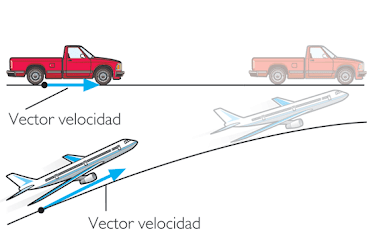
\includegraphics[scale=0.4]{images/vectorvelocidad.png}
 % cinematica.png: 0x0 px, 300dpi, 0.00x0.00 cm, bb=
 \caption{Ilustración del vector velocidad.}
\end{figure}

\textbf{Velocidad instantánea:}\\

 Es la que tiene el cuerpo en un instante específico, en un punto determinado de su trayectoria. Se define la velocidad 
instantánea o simplemente velocidad como el límite de la velocidad media cuando el intervalo de tiempo considerado tiende a 0. 
Esta velocidad es la que marca el velocímetro dentro de un auto por ejemplo.

 \begin{equation}
 \vec{v}=\lim_{\Delta t \to 0}\frac{\Delta \vec{r}}{\Delta t}\quad [m/s]
 \end{equation}

Una vez comprendido estos conceptos fundamentales del movimiento es tiempo de analizar el movimiento más simple que existe: 
\textit{El movimiento rectilíneo}.

\subsection*{Problemas}

\begin{enumerate}
 \item ¿Cuál es el desplazamiento realizado por un móvil que partió desde la posición $\vec{r_0} = 20 km;N34^\circ O$ hacia la 
posición $\vec{r_f} = 30 km; S45^\circ E$? 

\item Si el desplazamiento realizado por el móvil del problema anterior fue realizado en un tiempo promedio de 4 minutos,¿cuál es 
la velocidad promedio desarrollada por dicho móvil?

\end{enumerate}


\chapter{Movimiento Rectilíneo:}

\textit{``Al principio vienen necesariamente a la mente la fantasía y la fábula. Desfilan después los cálculos matemáticos, y 
solo 
al final la realización corona el pensamiento.''} \textbf{Konstantin Tsiolkovski.} 
\vspace{1.0 cm}

Un movimiento es rectilíneo cuando describe una trayectoria recta. En ese tipo de movimiento la aceleración y la velocidad son 
siempre paralelas. Usualmente se estudian dos casos particulares de movimiento rectilíneo: Uniforme y el uniformemente variado.

\section{Movimiento Rectilíneo Uniforme (MRU):}
 
Es el movimiento en que un cuerpo móvil se mueve a tráves de una trayectoria recta (una línea recta) y con una velocidad 
constante; lo que implica que este cuerpo con este tipo de movimiento recorre distancias iguales en tiempos iguales.Esto implica 
que la velocida en cualquier instante cualesquiera siempre
 tendrá el mismo valor.\\

En este movimiento apenas se tiene una ecuación de movimiento:

\begin{equation}
 v = \frac{d}{t}\quad [m/s]
\end{equation}

donde $v$ es la velocidad del cuerpo, $d$ la distancia recorrida y $t$ el tiempo recorrido para cubrir dicha distancia. Y de 
forma vectorial se tiene que:

\begin{equation}
 \vec{v} = \frac{\Delta\vec{r}}{\Delta t}
\end{equation}

es de notar que como el movimientoes rectilíneo la distancia recorrida por el cuerpo coindide con el módulo del vector 
desplazamiento del movimiento.\\
 
\begin{figure}[ht]
 \centering
 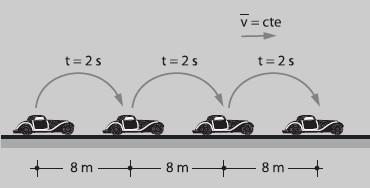
\includegraphics[scale=0.8]{images/Movimiento_rectilineo_uniforme.jpg}
 % cinematica.png: 0x0 px, 300dpi, 0.00x0.00 cm, bb=
 \caption{Ilustración del vector velocidad.}\label{mru}
\end{figure} 
 
La ilustración \ref{mru} muesta a un auto con MRU que cada 2 segundos recorre una distancia de 8 metros, esto  corresponde a 
decir que su velocidad es de $v = \frac{8m}{2s} = 4 m/s$, por lo cual despues de 6 segundos el auto habrá recorrido 24 metros.

\subsection{Problemas de mru}

\begin{enumerate}

\item Encuentre la longitud recorrida por un móvil que va a una velocidad de 1200 cm/s durante
 media hora. 

\item Un tren va a una velocidad de 200 km/h.
 ¿Qué distancia recorrerá en media hora? 

\item Calcula la velocidad expresada en unidades el SI de un camión que recorre los 90 km que
 existe entre dos ciudades 
separadas en 1 hora y 10 minutos. 

\item  Un automóvil recorre 180 m en 30 segundos. ¿Cuál es su
 velocidad? 

\item  Una partícula situada en el punto 
 (3,-4)m se mueve con velocidad constante hasta el punto (4,5)m en 12 segundos, 
determina la 
velocidad empleada

\item  Dos autos de carrera compiten entre si
 en una pista en
 línea recta cuya longitud es de 30 km. ¿Cuál será el auto 
ganador si el primero tiene una
 velocidad de 144 km/h, mientras que el segundo tiene una velocidad de 300 km/h pero

parte desde una posición de ventaja de 500 m?

\item Un coche se mueve durante 30 minutos a 40 km/h;
 después se mueve a 60 km/h durante la siguiente hora. Finalmente durante 
15 minutos
 circula a 20 km/h. ¿Qué distancia total habrá recorrido?
 
\item En el mismo instante, una motocicleta sale de la ciudad A y otra de la ciudad B, con la intención de encontrarse en el 
camino recto de 60 kilómetros que une ambas ciudades. Sabiendo que las velocidades de las motocicletas son 70km/h y 55km/h, 
calcular cuánto tardarán en encontrarse.

\item En una persecución policial, el automóvil a la fuga lleva una velocidad de 150km/h cuando
 pasa por un determinado punto 
de una carretera. Tres minutos después, el automóvil oficial que sigue al
 anterior pasa por dicho punto a una velocidad de tan 
solo 240km/h para evitar causar un accidente con los
 demás vehículos de la carretera a causa de un exceso de velocidad. Se 
supone que las velocidades indicadas
 son constantes y la carretera es recta. Calcular cuánto tardará la policía en alcanzar 
al delincuente.


\item Para recorrer dos puntos que distan entre sí 200 m, un
 móvil se desplaza con una velocidad constante de 50 m/s, si se 
duplica su velocidad para
 cubrir la misma distancia , ¿cuántos segundos utilizará?

\item  Dos autos de carrera compiten entre si
 en una pista en
 línea recta cuya longitud es de 30 km. ¿Cuál será el auto 
ganador si el primero tiene una
 velocidad de 144 km/h, mientras que el segundo tiene una velocidad de 300 km/h pero

parte desde una posición de ventaja de 500 m?

\item  La velocidad de la luz en el vacío es, 
aproximadamente, v = 300.000 km/s. ¿Cuánto tarda en llegar la luz del Sol al 
planeta Tierra si éstos 
distan unos 149,6 millones de kilómetros?


\item  Dos trenes parten de una misma
 estación; uno a 50 km/h y el otro a 72 km/h. ¿A qué distancia se encontrarán al cabo de 
media
 hora si marchan en sentido contrario? 


\item  ¿En que momento se cruzan dos 
 autos que parten de dos ciudades que distan 80 km, si sus velocidades son de 70 km/h y 90 
km/h, 
respectivamente y que van al encuentro del uno con respecto al otro?

\item  Un auto viaja con MRU y debe llegar a su destino a las
 8.00 PM. Si viajara a 140 km/h llegarııa una hora después y si 
viajara a 180 km/h llegaría
 media hora antes. ¿A qué velocidad debe el auto viajar para que llegar a la hora indicada?

\item Dos
 móviles están separados 200 km, y se mueven al encuentro llegando a cruzarse al cabo
 de 8 horas. Calcula la velocidad 
del más veloz, si la velocidad del otro es 2 km/h menos. 
\end{enumerate}


\section{Movimiento Rectilíneo Uniformemente Variado:}
 
En este movimiento al contrario que el MRU la velocidad con la que se mueve el móvil ya no es constante en el tiempo, y existe 
una nueva cantidad cinemática que da de cuenta de este cambio llamada \textit{aceleración}. 

\subsection{La aceleración:}

La aceleración $a$ es una cantidad vectorial que mide el ritmo de cambio de la velocidad con respecto al tiempo. Es decir, esta 
cantidad es una medida de como cambia la velocidad del móvil. Y esta cantidad se calcula así:

\begin{equation}
 \vec{a}=\frac{\Delta \vec{v}}{\Delta t}\quad [m/s^2] 
 \end{equation}
 
siendo $\Delta \vec{v}=\vec{v_f}-\vec{v_0}$ la diferencia entre velocidades (desde una velocidad inicial $\vec{v_0}$ hasta una 
velocidad final $\vec{v_f}$) realizado por el cuerpo en el intervalo de tiempo $\Delta t$.\\

La principal característica del MRUV es que posee una aceleración que es constante en el tiempo, es decir, la aceleración del 
cuerpo con MRUV siempre tendrá el mismo valor para cualquier instante de tiempo. Por ejemplo la caída libre de un cuerpo, con 
aceleración de la gravedad constante.\\

El movimiento rectilíneo uniformemente variado puede ser acelerado o desacelerado (retardado):\\

\textbf{Acelerado:} El movimiento es acelerado cuando la aceleración que experimenta el cuerpo en movimiento es de signo positivo 
($a > 0$), y esto quiere decir que con el paso del tiempo el cuerpo se ``acelera'': su velocidad va aumentando en el tiempo.\\

\textbf{Retardado:} Es cuando la aceleración que experimenta el cuerpo en movimiento es de signo negativo ($a < 0$), y esto 
quiere decir que con el paso del tiempo el cuerpo se ``desacelera'' o se ?frena?: su velocidad va disminuyendo en el tiempo.\\

\begin{figure}[ht]
 \centering
 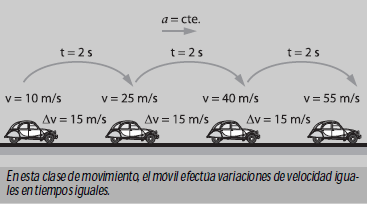
\includegraphics[scale=0.7]{images/mruv.png}
 % cinematica.png: 0x0 px, 300dpi, 0.00x0.00 cm, bb=
 \caption{Ilustración de una automóvil con MRUV.}\label{mruv}
\end{figure} 

En la figura \ref{mruv} se observa como un automóvil con MRUV cada 2 segundos incrementa su velocidad en $\Delta v = 15 m/s$, y 
así por tanto su aceleración es $a = \frac{\Delta v}{\Delta t} = \frac{15 m/s}{2s} = 7.5 m/s^2$, y como en este caso como $a>0$ 
se trata de un movimiento acelerado.\\

Este movimiento esta regido por cuatro ecuaciones de movimiento siguientes:

\begin{equation}
 v_f = v_o + at
\end{equation}

\begin{equation}
 v_f^2 = v_0^2 + 2ad
\end{equation}

\begin{equation}
 d = (\frac{v_f+v_0}{2})t
\end{equation}

\begin{equation}
 d = v_0t+ \frac{1}{2}at^2
\end{equation}

Dónde: $v_f$ : es la velocidad final del cuerpo en movimiento (se mide en $[m/s]$), $v_0$ : es la velocidad inicial del cuerpo en 
movimiento (se mide en $[m/s]$), $a$ : es la aceleración del cuerpo en movimiento (se mide en $[m/s 2]$), $t$: es el tiempo que 
emplea el cuerpo durante el movimiento (se mide en $[s]$), d: es la distancia recorrida por el cuerpo (se mide en $[m]$). Estas 
ecuaciones están planteadas de forma escalar, es decir, relacionan los módulos de las magnitudes vectoriales del cuerpo en 
movimiento, pero es importante notar que estas ecuaciones también se pueden plantear de forma vectorial de la siguiente manera: 

\begin{equation}
\vec{v_f} = \vec{v_0} + \vec{a}t 
\end{equation}

\begin{equation}
 v_f^2 = v_0^2+2a\Delta r
\end{equation}

\begin{equation}
 \Delta \vec{r} = (\frac{\vec{v_f}+\vec{v_0}}{2})t
\end{equation}

\begin{equation}
 \Delta \vec{r} = \vec{v_0}t + \frac{1}{2}\vec{a}t^2
\end{equation}
 
Observando detenidamente estas ecuaciones se infiere que cada ecuación tiene cuatro diferentes magnitudes relacionadas 
a través de ella, y por tanto conocer cualquiera de ella está en función de las otras tres, es decir, es suficiente con 
este tipo de ecuaciones encontrar una magnitud conociendo otras tres distintas (este es un dato importante en el momento de 
resolver problemas relacionados con el MRUV).

\subsection{Problemas de mruv}

\begin{enumerate}
 \item Un ciclista que está en reposo comienza a pedalear hasta alcanzar los 6 m/s en 6 minutos. Calcular la distancia total que 
recorre si continúa acelerando durante 5 minutos más.

\item  Un cuerpo se mueve con una velocidad de $3 \vec{i} – 4\vec{j}$ [m/s] y
 se le aplica una aceleración de $0.3 m/s^2$

 en la misma dirección de la velocidad. Determine la
 distancia recorrida al cabo de un minuto de recorrido.

 
\item Dos vehículos separados por 20 km parten al encuentro
 en el instante t=0. El primero lo hace con una velocidad inicial 
constante de 20 km/h. El
 segundo parte desde el reposo y con una aceleración de $0,5 m/s^2$. ¿A qué distancia de la
 salida del 
primer vehııculo se encuentran? 

\item Un móvil viaja a 60 km/h y comienza a reducir su velocidad a partir del instante t=0. Al
 cabo de 8 segundos se detiene 
completamente. ¿Cuál fue aceleración durante el período en el que redujo su
 velocidad?

\item Un tren viaja a 80 km/h. Inmediatamente después de pasar una señal en rojo comienza a
 detenerse. Se detiene completamente 
a los 150 metros. Determinar su aceleración.

\item Un automóvil corre a una velocidad 
 de 20 m/s, en ese instante pisa el acelerador produciendo una aceleración constante 
que aumenta 
su velocidad a 30 m/s en 5s. ¿Cuál será su velocidad al cabo de 10s?

\item Un móvil se desplaza con velocidad inicial desconocida. A partir de t=0 comienza a acelerar
 a $1,7 m/s^2$
. Luego de 12 
segundos se desplaza a 110 km/h. Determinar la velocidad inicial.

\item Un tren viaja a una velocidad constante de 90 km/h y pasa una señal en rojo. A 80 metros
 de pasar la señal comienza a 
reducir su velocidad a razón de $3m/s^2$
. ¿A qué distancia de la señal se detiene
 por completo?¿Cuánto tarda en hacerlo a 
partir del momento en el que pasa la señal?

\item Dos vehículos separados por 20 km parten al encuentro en el instante t=0. El primero lo
 hace con una velocidad inicial 
constante de 20 km/h. El segundo parte desde el reposo y con una aceleración
 de $0,5 m/s^2$
 . ¿A qué distancia de la salida 
del primer vehículo se encuentran?

\item Dos vehículos A y B se mueven con aceleración
 constante, el vehículo B tiene una velocidad inicial $\vec{v_0B} = (50 
\vec{i} – 4 \vec{j}) km/h$, y después de 2
 horas alcanza una velocidad final $\vec{v_fB}=(54 \vec{i} + 16\vec{j}) km/h$. Si se 
conoce que la aceleración
 del vehículo A es el doble que la del vehículo B, determine la aceleración del vehículo A.



\end{enumerate}


\section{Caída libre y lanzamiento vertical de los cuerpos:}

Un caso especial de MRUV es el movimiento de los cuerpos cuando están exclusivamente sólo bajo la influencia de la fuerza de la 
gravedad. También en este apartado se supondrá que la resistencia aerodinámica del aire es insignificante (para el caso real esto 
depende de la forma del cuerpo), es decir, se supone que el cuerpo se mueve el vacío. 

\subsection{Caída libre:}

Se trata del movimiento de un cuerpo cuando cae desde cierta altura (la distancia que recorre el cuerpo durante toda la caída) 
por encima del nivel de la superficie de la Tierra (piso) hacia abajo. Este movimiento es un MRUV con una aceleración la cual es 
la gravedad $a = g = 9.8 m/s^2$ (constante), la cual está en la misma dirección de la velocidad lo cual hace que se trate de un 
movimiento acelerado. 

\begin{figure}[ht]
 \centering
 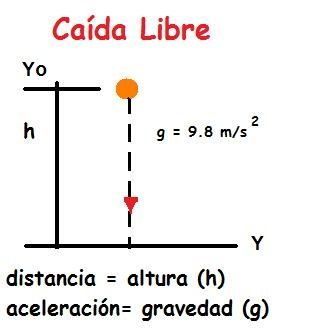
\includegraphics[scale=0.5]{images/caida-libre.jpg}
 % cinematica.png: 0x0 px, 300dpi, 0.00x0.00 cm, bb=
 \caption{Ilustración de la caída libre de un cuerpo.}\label{caidalibre}
\end{figure} 

Y las ecuaciones de movimiento son las de un MRUV:

\begin{equation}
 v_f = v_0 + gt
\end{equation}

\begin{equation}
 v_f^2 = v_0^2 + 2gh
\end{equation}

\begin{equation}
 h = (\frac{v_f + v_0}{2})t
\end{equation}

\begin{equation}
 h = v_0t + \frac{1}{2}gt^2
\end{equation}

En la figura \ref{caidalibre2} se observa como un cuerpo parte del reposo ($v_0 = 0$) y cae bajo la acción de la gravedad y 
consecuentemente su velocidad va aumentado rápidamente con el paso del tiempo.
 
\begin{figure}[ht]
 \centering
 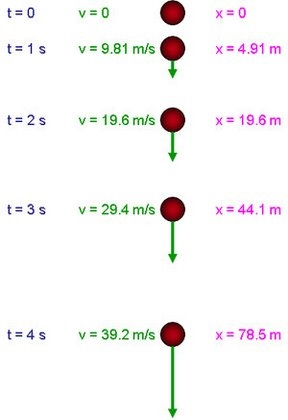
\includegraphics[scale=0.4]{images/freefall-timeline-large.jpg}
 % cinematica.png: 0x0 px, 300dpi, 0.00x0.00 cm, bb=
 \caption{Ilustración del tiempo de caída de un cuerpo.}\label{caidalibre2}
\end{figure}  
 
\subsection{Lanzamiento vertical:}

Este movimiento es de tipo MRUV que trata del lanzamiento de un cuerpo en línea recta hacia arriba en contra de la gravedad, y 
por tanto en este caso para cálculos la gravedad se toma como $g = -9.8 m/s^2$, se nota el signo negativo por cuanto en este caso 
el movimiento es retardado y la fuerza de la gravedad está encontra del movimiento. Obviamente para que ocurra este movimiento el 
cuerpo lanzado debe partir con una velocidad inicial diferente de cero ($v_0 = 0$), y así mismo la velocidad alcanzará su valor 
mínimo de cero donde se dice que el cuerpo ha alcanzado su altura máxima ($h_{max}$) y ya no sube más, y posteriormente bajará 
con 
un movimiento de caída libre que parte del reposo.
 
\begin{figure}[ht]
 \centering
 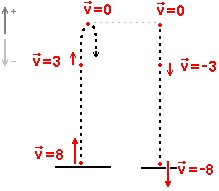
\includegraphics[scale=0.7]{images/lanzamientovertical.jpg}
 % cinematica.png: 0x0 px, 300dpi, 0.00x0.00 cm, bb=
 \caption{Ilustración del lanzamiento vertical.}\label{lanzamientov}
\end{figure}   
 
Es importante mencionar que cuando cuerpo realiza un lanzamiento vertical, este movimiento tiene cierta simetría con la caída 
libre que luego realizará una vez que alcanze la altura máxima, debido a que esta bajo la mismo módulo de la aceleración de la 
gravedad y que además recorre la misma distancia (altura), y por tanto el tiempo que demorá en subir el cuerpo (tiempo de subida: 
$t_s$) es el mismo tiempo que demora en bajar (tiempo de bajada: $t_b$).

\subsection{Problemas de caída libre y lanzamiento vertical}

\begin{enumerate}
 \item Supongamos que arrojamos una piedra hacia arriba, ¿a que velocidad la tenemos que lanzar para que alcance una altura máxima
de 32 metros?
\item Hallar la velocidad con que fue lanzado un cuerpo hacia arriba si ésta se reduce a la tercera parte cuando ha subido 29.4 m.
\item Un tipo está parado a 20 m de altura. Calcular qué tiempo tarda y con qué velocidad toca el suelo una piedra si el tipo:
\begin{itemize}
 \item[a.] La deja caer.
 \item[b.] La tira para abajo con V0 = 10 m/s.
\end{itemize}
\item Se lanza un cuerpo hacia arriba con una velocidad de 24,5 m/s desde un punto a 68,6 metros por encima del suelo. Halla:

\begin{itemize}
 \item[a.] La altura máxima que alcanza el cuerpo.
 \item[b.] El tiempo necesario para volver al punto de lanzamiento.
 \item[c.] La velocidad de llegada al suelo.
 \item[d.] El tiempo total en el aire.
\end{itemize}

\item Determina la velocidad con que fue lanzado un cuerpo hacia arriba si ésta se reduce a la tercera 
parte cuando ha subido 
29.4 m.

\item  Se deja caer una
 piedra desde lo alto de un edificio de 40 m de altura, ¿con que velocidad llegará al suelo?

\item  Una piedra es lanzada verticalmente
 hacia arriba con una velocidad de 98 m/s. ¿A qué altura llegará?

\item Un cuerpo se lanza verticalmente hacia arriba desde una ventana y luego de 4 segundos triplica su velocidad. Hallar la 
máxima altura alcanzada por el cuerpo respecto al lugar de lanzamiento.
\item Una esfera se deja caer desde 80 m de altura y al rebotar en el piso se eleva siempre la cuarta parte de la altura 
anterior. 
¿Qué tiempo ha transcurrido hasta que se produce el tercer impacto?.
\item Un cuerpo cae libremente desde el reposo. La mitad de su caída se realiza en el último segundo, calcular el tiempo total.

\item Un cuerpo se suelta desde una altura H. ¿Con qué velocidad llegará al suelo?.

\item Desde la boca de un pozo de 50 metros de profundidad, ¿a qué velocidad hay que lanzar una
 piedra para que llegue al fondo 
en 2 segundos?

\item Lanzamos hacia arriba un objeto desde la altura de 1,5 m y con una velocidad de 24,5 m/s.
 Determina la posici´on y la 
velocidad al instante de 3 segundos.


\item  Un cuerpo parte del reposo con una aceleración de $5 m/s^2$
.
 ¿Cuál es la distancia recorrida durante el octavo segundo 
del recorrido?

\item  Un niño deja caer una piedra desde lo alto de un árbol de 5
 m del suelo. Simultáneamente, otro niño lanza una piedra 
desde el suelo hacia arriba con una
 velocidad de 3 m/s. ¿A qué distancia del suelo coinciden las dos piedras en sus respectivas

trayectorias?

\item  Desde una altura de 200
 m se deja caer un cuerpo, y simultáneamente desde el suelo se lanza un cuerpo con una
 velocidad 
de 20 m/s hacia arriba. ¿Cuándo la distancia entre ellos es de 20m?.


\item Un niño deja caer una piedra desde lo alto de un árbol de 4 m del suelo. Simultáneamente,
 otro niño lanza una piedra desde 
el suelo hacia arriba con una velocidad de $6 m/s$
. ¿A qué distancia del
 suelo coinciden las dos piedras en sus respectivas 
trayectorias?

\item A una niña se le cae una pelota desde el quito piso de un edificio, a 15 metros del suelo.
 El vecino del tercero, a 9 m 
del suelo la ve pasar. Calcular: a) El tiempo que tarda en llegar al suelo, b) su
 velocidad al pasar por el tercer piso.


\item Nahiara deja caer una moneda a un pozo y escucha el sonido del agua 2,5 s después de
 iniciarse la caída. Halla: a) La 
profundidad del pozo y, b) la velocidad con la que llega al agua (La velocidad del sonido $340 m/s$).

\end{enumerate}


\chapter{Movimiento parabólico:} 
 
\textit{``¿Por qué las cosas son como son y no de otra manera?''} \textbf{Johannes Kepler}
\vspace{1.0cm}  
 
También llamado tiro de proyectiles, corresponde al movimiento de un proyectil en el campo gravitatorio y que cuya  trayectoria 
es 
una parábola.
 
\begin{figure}[ht]
 \centering
 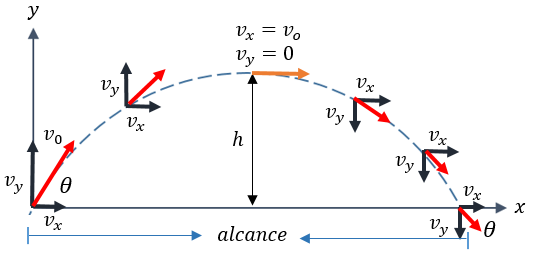
\includegraphics[scale=0.6]{images/movimiento_parabolico.png}
 % cinematica.png: 0x0 px, 300dpi, 0.00x0.00 cm, bb=
 \caption{Ilustración del movimiento parabólico.}\label{movparabola}
\end{figure}   

Para el análisis de este movimiento se lo considera como la composición de dos movimientos: horizontal (respecto al eje x) y 
vertical (respecto al eje y).\\

Antes de analizar estos submovimientos hay que considerar que el móvil inicia su movimiento con una velocidad inicial $\vec{v_0}$ 
que hace un ángulo $\theta$ (ángulo de tiro) con la horizontal referenciada con el eje x positivo. Así, resulta conveniente 
encontrar las componentes de esta velocidad en cada eje cartesiano, y estas son:

\begin{equation}
 \vec{v_{0x}}=\vec{v_0}cos(\theta)
\end{equation}

\begin{equation}
 \vec{v_{0y}}=\vec{v_0}sen(\theta)
\end{equation}

\textbf{Movimiento horizontal:}\\

Este movimiento se refiere al movimiento de la proyección del cuerpo en el eje $x$, en este eje la velocidad es constante, es 
decir, $\vec{v_{0x}} =  \text{constante} = v_x$ y por tanto el movimiento en este eje es MRU, y por tanto la ecuación de 
movimiento es:

\begin{equation}
 x = v_{0x}t=v_x \Delta t
\end{equation}

A la distancia máxima en el eje $x$ que la proyección del cuerpo logra moverse se la denomina alcance máximo ($x_{max}$). Y al 
tiempo que demoró en cubrir esa distancia se la llama tiempo de vuelo ($t_v$), con lo cual alcance máximo es:

\begin{equation}
 x_{max} =  v_x t_v
\end{equation}

\textbf{Movimiento vertical:}\\

Este es el movimiento correspondiente en el eje $y$, en este movimiento se considera la acción de la gravedad ($g$), además, hay 
que distinguir que el movimiento se divide en dos etapas: la primera en la que el cuerpo sube con una velocidad inicial $v_{0y} = 
 v_0 sen(\theta)$ y llega a una altura máxima $h_{max}$ donde el cuerpo tiene una velocidad en $y$ de 0 (en esta etapa se ha 
realizado un lanzamiento vertical), luego en el cuerpo cae con una velocidad inicial en $y$ de cero así que cae realizando una 
caída libre.\\

Entonces la velocidad del cuerpo en cualquier instante es:

\begin{equation}
 \vec{v} = \vec{v_x} + \vec{v_y}\quad \text{cuyo módulo es:} \quad v = \sqrt{v_x^2+v_y^2}
\end{equation}

Debido a la simetría del movimiento en el eje $y$ es notorio que el tiempo de vuelo es el doble del tiempo de subida como el 
tiempo de bajada.

\begin{equation}
 t_v = 2t_s =2t_b
\end{equation}

Además, que las ecuaciones de movimiento en el eje de las $y$ son las de lanzamiento vertical y caída libre respectivamente:

\begin{equation}
 v_{fy} = v_{0y} + gt
\end{equation}

\begin{equation}
 v_{fy}^2 = v_{0y}^2 + 2gh
\end{equation}\label{dos}

\begin{equation}
 h =(\frac{v_{fy}+v_{oy}}{2})t
\end{equation}

\begin{equation}
 h = v_{oy}t + \frac{1}{2}gt^2
\end{equation}

Y así por tanto para encontrar por ejemplo la altura mámixa se utiliza la ecuación (\ref{dos}) sabiendo que la $v_{fy} = 0$, así 
que:

\begin{equation}
 h_{max} = -\frac{v_0^2sen^2(\theta)}{2g}
\end{equation}

\section{Problemas de movimiento parabólico}

\begin{enumerate}

 \item Un soldado acostado en el suelo lanza una granada con velocidad inicial de 25 m/s, y un ángulo de elevación de
 $53^\circ$. Despues de que tiempo escuchará el estallido. Velocidad del sonido: 340m/s.
 
 \item Se dispara una flecha a 25 m/s y a $30^\circ$ con la horizontal,
 para dar en un árbol que está a 30 metros de distancia. 
Determinar: a) la altura a la que se elevará
 la flecha,  b) el ángulo que formarán la
 flecha con el árbol, y c) el tiempo que 
tarda la flecha hasta dar con el árbol. 


\item Un jugador de Fútbol Americano patea el balón con una velocidad de 30 m/s, y éste mismo
 lleva un ángulo de elevación de 
$45^\circ
$ respecto a la horizontal. Calcule; a) altura, b) alcance, y c) tiempo que
 permanece en el aire.

\item  Un proyectil es lanzado de modo que su alcance máximo
 es de 44 m. Sabiendo que el ángulo de tiro es de $45^\circ$, 
averigua la velocidad inicial del
 lanzamiento. 

\item Se dispara un proyectil con una velocidad inicial de 50 m/s
 y un ángulo de $25^\circ$, por encima de la horizontal. 
Calcular la velocidad del proyectil después de
 los 6s.

\item Se dispara un proyectil con una velocidad inicial de 60 m/s y un ángulo de $30^\circ
$, por encima de
 la horizontal. 
Calcular: a) Posición y velocidad después de los 6s, b) tiempo para alcanzar la altura máxima
 y c) el  alcance horizontal.

\item  Un proyectil es lanzado de modo que su alcance máximo
 es de 55 m. Sabiendo que el ángulo de tiro es de $45^\circ$, 
averigua la velocidad inicial del
 lanzamiento. 

\item Dos personas, A y B, se encuentran en las ventanas de dos edificios ubicados uno frente a
 otro, en los lados opuestos de 
una calle. Los edificios est´an separados entre sí 10 m y las alturas de las
 ventanas respecto al piso son 15 m para A y 20 m 
para B. Si B lanza, hacia la derecha, un globo con agua
 con la intención de impactar a A y la rapidez inicial del globo es de 
10 m/s, calcule: a) el ángulo de disparo
 respecto a la horizontal, y b) el vector velocidad del proyectil el momento del impacto.

\end{enumerate}


\chapter{Movimiento circular:}

\textit{``Y, lógicamente, se mueve con movimiento incesante: pues todas las cosas cesan de moverse cuando llegan a su lugar 
propio, mientras que el lugar de donde parte el cuerpo circular es el mismo adonde va a parar.''} \textbf{Aristóteles}
\vspace{1.0cm}

El movimiento circular es el que recorre una partícula o cuerpo realizando una circunferencia como trayectoria. Este movimiento 
tiene un eje y todos los puntos por los que pasa la partícula se encuentran a una distancia constante (R: radio de la 
circunferencia) del eje. De modo que cuando el cuerpo con movimiento circular se mueve recorre un longitud de arco ($s$) 
sostenido por un ángulo recorrido $\theta$, y así se tiene que:

\begin{equation}
 s = R\theta
\end{equation}

donde la longitud de arco $s$ se mide en metros, $R$ es el radio de la circunferencia y el ángulo recorrido $\theta$ se mide en 
radianes.\footnote{Los grados sexagésimales se convierten a radianes mediante el uso de la equivalencia de: $360^\circ = 2\pi 
rad$.}

\begin{figure}[ht]
 \centering
 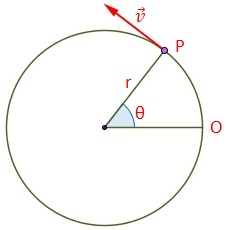
\includegraphics[scale=0.6]{images/movimiento-circular.jpg}
 % cinematica.png: 0x0 px, 300dpi, 0.00x0.00 cm, bb=
 \caption{Ilustración del movimiento circular.}\label{circular}
\end{figure}   

Ya que el cuerpo se mueve a tráves de la trayectoria circular posee dos velocidades: una angular y otra lineal.\\

\subsection{Velocidad angular:}

Esta velocidad mide el ritmo de cambio del ángulo recorrido por el cuerpo en movimiento con respecto al tiempo:

\begin{equation}
\omega = \frac{\Delta \theta}{\Delta t} \quad [rad/s]
\end{equation}

\subsection{Velocidad Lineal:}

También llamada velocidad tangencial mide el ritmo de cambio de la longitud de arco recorrida por el cuerpo con respecto al 
tiempo.

\begin{equation}
v = \frac{\Delta s}{\Delta t} = \frac{R\Delta \theta}{\Delta t} = R\omega \quad [m/s]
\end{equation}

Esta velocidad depende exclusivamente de la velocidad angular de manera directa.\\

También se definen dos magnitudes importantes para este movimiento:\\

\textbf{Período:} es el tiempo $T$ que tarda la partícula en dar una vuelta a la circunferencia completa.\\

\textbf{Frecuencia:} Es el número de vueltas $f$ que recorre la partícula en una unidad de tiempo. Se expresa en ciclos/s o 
hertzios (Hz).\\

Estas dos cantidades se relacionan de manera inversa:

\begin{equation}
f = \frac{1}{T}\quad [Hz]
\end{equation}
, y también con la velocidad angular: 
\begin{equation}
w = 2\pi f = \frac{2\pi}{T}
\end{equation}

Cuando un móvil se mueve con movimiento circular su velocidad lineal siempre esta en constante cambio de dirección, y como se 
sabe que siempre el cambio de velocidad en el tiempo esta medido por una aceleración, y esta aceleración se llama aceleración 
centrípeta.

\subsection{Aceleración centrípeta:}

\begin{figure}[ht]
 \centering
 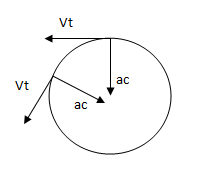
\includegraphics[scale=0.6]{images/aceleracion-centripeta.jpg}
 % cinematica.png: 0x0 px, 300dpi, 0.00x0.00 cm, bb=
 \caption{Ilustración de a aceleración centrípeta.}\label{ac}
\end{figure}

Esta aceleración es la que se origina debido al cambio de dirección constante de la velocidad lineal cuando el cuerpo gira a 
través de la circunferencia, y su dirección es central, siempre apuntando al centro del círculo. Y su expresión de cálculo es:

\begin{equation}
a_c = \frac{v^2}{R} =  \omega^2 R\quad [m/s^2]
\end{equation}

\begin{figure}[ht]
 \centering
 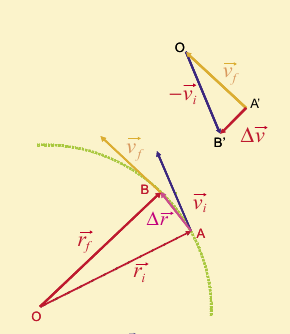
\includegraphics[scale=0.6]{images/acentripeta.png}
 % cinematica.png: 0x0 px, 300dpi, 0.00x0.00 cm, bb=
 \caption{Ilustración del origen vectorial de la aceleración centrípeta.}\label{ac}
\end{figure} 

\section{Movimiento Circular Uniforme (MCU):}

Es aquel movimiento circular en que el móvil se mueve con velocidad tanto angular y lineal constante, es decir la velocidad 
angular y la lineal no cambian su valor en el tiempo. De este modo se puede decir que el móvil en este movimiento recorre 
distancias iguales en tiempo iguales. 

\begin{tcolorbox}
Es decir, en el MCU: $\omega = constante$ y $v = constante.$
\end{tcolorbox}

Esto implica que el cuerpo que tiene MCU sólamente posee una aceleración que es la centrípeta.

\subsection{Problemas de mcu}

\begin{enumerate}
\item Tranformar los siguientes ángulos en radianes:
\begin{itemize}
 \item[a.] $40^\circ$
 \item[b.] $140^\circ$
 \item[c.] $155^\circ$
 \item[d.] $640^\circ$
 \item[e.] $60^\circ$
 \item[f.] $40^\circ$
 \item[g.] $55^\circ$
 \item[h.] $64^\circ$
\end{itemize}

 \item Encontrar la longitud de arco de circunferencia de radio y ángulo:
\begin{itemize}
 \item[a.] 20 cm y $45^\circ$
 \item[b.] 5.0 km y $75^\circ$
 \item[c.] 30 m y $360^\circ$
 \item[d.] 6.5 m y $60^\circ$
  \item[e.] 200 cm y $45^\circ$
 \item[f.] 50.0 km y $75^\circ$
 \item[g.] 77 cm y $360^\circ$
 \item[h.] 50 mm y $60^\circ$
\end{itemize}

\item Una partícula gira por una trayectoria circular de radio 1m da 40 vueltas en 6 segundos. Calcular: a) la velocidad angular 
y b) la aceleración centrípeta.

\item  Una partícula gira por una trayectoria circular de radio 1m da 40 vueltas en 6 segundos. Calcular: a) la velocidad 
angular y b) la aceleración centrípeta.

\item  Un móvil se mueve en una circunferencia de 50 cm de radio con una velocidad angular de 180 rpm, determine la distancia 
recorrida y la frecuencia alcanzada después de 10s.


\item  Del problema anterior encuentre lo siguiente: a) La frecuencia y b) el ángulo girado luego de un minuto.


\item Un punto de la periferia de la rueda de un automóvil con radio 0,30 m se mueve con una velocidad de 36 km/h. ¿Cuál es su 
velocidad angular en rad/s? ¿Cuál es su aceleración centrípeta? 

\item Las aspas de un ventilador giran uniformemente a razón de 90 vueltas por minuto. Determina: a) su velocidad angular, en 
rad/s; b) el número de vueltas que darán las aspas en 5min; c) Su periodo y d) su frecuencia.

\item Un móvil se mueve en una circunferencia de 50 cm de radio con una velocidad angular de 180 rpm/min, determine la distancia 
recorrida y la frecuencia alcanzada después de 10s

 \item Un ciclista recorre 5,4 km en 15 min a velocidad constante. Si el diámetro de las ruedas de su bicicleta es de 80 cm, 
calcula: a) la velocidad angular de las ruedas y b) el número de vueltas que dan las ruedas en ese tiempo.

\item Dos poleas de 6 y 15 cm de radio respectivamente, giran conectadas por una banda. Si la velocidad angular de la polea de 
menor radio es 20 vueltas/segundo. ¿Cúal es la velocidad angular de la polea de radio mayor?.
\begin{figure}[H]
 \centering
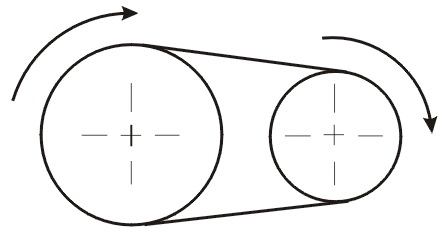
\includegraphics[width=5.0cm,height=3.0cm]{images/poleas.jpg}
\end{figure}

\item Un auto se mueve alrededor de una pista circular cuyo radio es de 50 metros de radio con un velocidad constante de 90 km/h.
 ¿Cuál es la velocidad angular que posee ese auto?
 
\item La rueda de una bicicleta tiene 30 cm de radio y gira uniformemente a razón de 25 vueltas por minuto. Calcula: a) La 
velocidad angular, en rad/s, b) La velocidad lineal de un punto de la periferia de la rueda, c) Ángulo girado por la rueda en 30 
segundos y d) número de vueltas en ese tiempo.

\item Un coche circula a una velocidad de 90 Km/h , si el radio de las ruedas del coche es de 30 cm, calcula: a)su velocidad 
lineal en m/s y b)la velocidad angular de las ruedas en rad /s y r.p.m.

\item  Si la velocidad angular de un disco se duplica, ¿Qué ocurre con la velocidad lineal?
 
\item Un astronauta da la vuelta a la Tierra cada 300 minutos.¿Cuál es la velocidad angular?¿Cuál es su velocidad lineal si 
describe una orbita de 30000 km de radio?

\item ¿Cuál es la velocidad de un angular de un disco que gira con una velocidad angular de 13,4 rad en un minuto? Si el radio 
del disco es 20 cm, ¿cuál es la velocidad lineal en el borde del mismo?.

\item ¿Cuánto tiempo necesitará el disco anterior para girar 3 vueltas enteras?¿Cuál es la aceleración centrípeta en el borde del 
disco?

\item ¿Cuál es la velocidad angular de un disco que gira con una velocidad angular de $3\pi$ rad en medio minuto? Si el radio del 
disco es 40 cm, ¿cuál es la aceleración centrípeta en el borde del mismo?.

\item ¿Cuál es la velocidad angular de las manecillas del reloj?¿El periodo del movimiento?

\item Un móvil recorre una circunferencia de 2 m de radio dando 20 vueltas en 10 segundos. Determinar:

\begin{itemize}
 \item [a.] La frecuencia.
 \item [b.] El periodo.
 \item [c.] La velocidad angular.
 \item [d.] La velocidad lineal.
\end{itemize}

\item Calcule la aceleración centrípeta de la   Luna.

\item Calcule la aceleración centrípeta y angular de la Tierra alrededor del Sol.

\item  Un punto de la periferia de la rueda de un automóvil con radio 0,30 m se mueve con una velocidad de 36 km/h. ¿Cuál es su 
velocidad angular en rad/s? ¿Cuál es su aceleración centrípeta?

\item Desde un mismo punto de la circunferencia parten dos móviles en sentido opuesto. El primero recorre la circunferencia en 
1h10 min y el segundo recorre un ángulo de $30^\circ$ en 3 segundos. Determine cuándo se encuentran los móviles.

\end{enumerate}


\section{Movimiento Circular Uniformemente Variado:}

Es el movimiento que realiza un cuerpo con trayectoria circular y con una aceleración tangencial, que hace que la velocidad 
lineal y angular no sean constantes en el tiempo. El cuerpo con MCUV tiene una aceleración angular y aceleración tangencial 
constantes, y estás miden la variación de la velocidad angular y lineal respecto al tiempo.\\

\subsection{Aceleración angular:}

Es una cantidad vectorial que mide el ritmo de cambio de la velocidad angular con el tiempo, la cual se mantiene constante en el 
MCUV. Esta aceleración se calcula así:

\begin{equation}
\alpha = \frac{\Delta \omega}{\Delta t} =  \frac{\omega_f - \omega_0}{\Delta t}\quad [rad/s^2]
\end{equation}
  

donde $\Delta \omega = \omega_f-\omega_0$ representa la variación de la velocidad angular desde una inicial $\omega_0$ hasta una 
final $\omega_f$. Si esta aceleración $\alpha$ es positiva el movimiento es acelerado, mientras que si $\alpha$ es negativa el 
movimiento es de frenado.

\subsection{Aceleración tangencial:}

O también llamada lineal, esta mide la variación de la velocidad tangencial con respecto al tiempo, la cual se mantiene constante 
en el MCUV. Esta aceleración se calcula así:

\begin{equation}
a_T =\frac{\Delta v}{\Delta t} =\frac{v_f-v_0}{\Delta t}\quad [m/s^2]
\end{equation} 

donde $\Delta v = v_f-v_0$ representa la variación de la velocidad tangencial desde una inicial $v_0$ hasta una final $v_f$. Si 
esta aceleración $a_T$ es positiva el movimiento es acelerado, mientras que si $\alpha$ es negativa el movimiento es de frenado. 
Así, mismo como la velocidad tangencial esta aceleración es tangente a la trayectoria, y mide de que tan rápido o tan lento el 
cuerpo está cambiando su velocidad.

\begin{tcolorbox}
En el MCUV: $a_T = constante$ y $\alpha = constante$
\end{tcolorbox}

Las dos aceleraciones anteriores descritas se relacionan mediante la siguiente ecuación:

\begin{equation}
a_T = \alpha R
\end{equation} 

, y la aceleración resultante de un cuerpo con MCUV es:

\begin{equation}
\vec{a} = \vec{a_T}+\vec{a_c}
\end{equation}

cuyo módulo es entonces:

\begin{equation}
a_R =\sqrt{a_c^2+a_T^2} 
\end{equation}

\begin{figure}[ht]
 \centering
 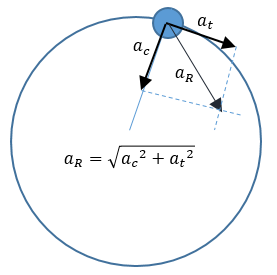
\includegraphics[scale=0.5]{images/aceleracion-resultante.png}
 % cinematica.png: 0x0 px, 300dpi, 0.00x0.00 cm, bb=
 \caption{Ilustración de la aceleración resultante en un MCUV.}\label{ac}
\end{figure} 
 
Este movimiento queda descrito completamente con las siguientes ecuaciones:\\

\textbf{Parte angular:}

\begin{equation}
\omega_f = \omega_0 + \alpha t
\end{equation}

\begin{equation}
\omega_f^2 = \omega_0^2 + 2\alpha\theta
\end{equation}

\begin{equation}
\theta = (\frac{\omega_f + \omega_0}{2})t
\end{equation}

\begin{equation}
\theta = \omega_0t+\frac{1}{2}\alpha t^2
\end{equation}

\textbf{Parte lineal:}

\begin{equation}
v_f = v_0 + a_Tt
\end{equation}

\begin{equation}
v_f^2 = v_0^2 +2a_Ts
\end{equation}

\begin{equation}
s = (\frac{v_f + v_0}{2})t
\end{equation}

\begin{equation}
s = v_0t+\frac{1}{2}a_Tt^2
\end{equation}


\section{Problemas de mcuv}

\begin{enumerate}

\item Una partícula inicia su M.C.U.V. con una velocidad tangencial de 6 m/s. Si su aceleración tangencial es $4 m/s^2$, y su 
radio de giro es 9 m. Determinar su velocidad tangencial y angular luego de 12 segundos.

\item Calcular la aceleración angular que tiene un disco, sabiendo que éste es capaz de triplicar la velocidad que tiene luego de 
dar 600 vueltas en 20 s.

\item La velocidad de una rueda, que gira con movimiento uniformemente retardado, disminuyó al ser frenada durante 1 minuto, 
desde 
300 R.P.M. hasta 180 R.P.M. Hallar la aceleración angular de la rueda.

\item Un ventilador alcanza su velocidad máxima de trabajo de 900 R.P.M. en 40 s. Si al ``encenderlo'' inicia su movimiento con 
aceleración constante, calcular cuántas revoluciones completa en el primer minuto de su movimiento.

\item La velocidad angular de un motor cambia uniformemente
 200 rpm a 120 rpm en 4 segundos. Determinar: a) la aceleración 
angular y b) el
 desplazamiento angular.

\item  La velocidad de
 un automóvil aumenta en 5 segundos de 15 km/h a 55 km/h. Si el radio de las ruedas es de 70
 cm, ¿cuál es 
la aceleración angular de las mismas? 

\item Un móvil tiene una velocidad tangencial de 120m/s; luego de 5 segundos esta velocidad se convierte en 154 m/s. Si el radio 
de la circunferencia es de 4m, hallar la aceleración angular. 

\item Una rueda de 50cm de diámetro tarda 10 segundos en adquirir una velocidad constante de 360rpm. Calcula la aceleración 
angular y la aceleración centrípeta que posee un punto en la periferia de la rueda a los 5 segundos la rueda del problema.

\item Un volante de 50cm de radio gira a 180 rpm. Si es frenado y se detiene en 20 segundos, calcula: a) La velocidad angular 
inicial en radianes por segundo, y b) La aceleración tangencial de frenado.

\item Calcular la  velocidad  angular  final  y  el desplazamiento  angular de  una  rueda  que  tiene una velocidad angular 
inicial de $8 rad/s$ y experimenta una aceleración de $3 rad/s^2$ en 12 s.

\item Una  rueda  gira  con  una  velocidad  angular inicial  de  12  rad/s  experimentando  una  aceleración de $5 rad/s^2$ en 
6s. Calcular: a) el desplazamiento angular total, b) la velocidad angular final.

\item La velocidad angular de un motor cambia uniformemente 200 rpm a 120 rpm en 4 segundos. Determinar la aceleración lineal de 
un punto que esta a 50 cm del eje de rotación del motor.

\item Un punto de la periferia de la rueda de un automóvil con radio 0,30 m  se mueve con una velocidad de 72 km/h, de pronto el 
automóvil se frena uniformemente a razón de $4 m/s^2$.  Calcular  el ángulo girado  después de 10 segundos.

\item  Un motor que tiene 
una frecuencia de 20 Hz, se apaga y se detiene en 5 segundos. ¿Cuál es su velocidad lineal al 

tiempo de 2 segundos de un punto que se ubica a 50 cm del eje de rotación del motor?

\end{enumerate}


\chapter{Dinámica}

\textit{``Si he realizado descubrimientos invaluables ha sido más por tener paciencia que cualquier otro talento.''}\textbf{Sir 
Isaac Newton}
\vspace{1.0cm}

En este apartado se refiere a la Dinámica, la cual es la parte de la Física que estudia o analiza el movimiento desde sus causas 
(fuerzas), es decir, que es lo que genera el movimiento.\\

Las causas que generan el movimiento se denominan fuerzas, entiendiéndose como fuerza a aquella capacidad física que ejerce un 
cuerpo sobre otro y que genera movimiento e incluso deformaciones.\\

La persona que realizó un estudio formidable acerca de Dinámica fue Sir Isaac Newton, y sobre cuyo estudio plasmado en tres leyes 
descansa la base de la Dinámica.
 
\section{Las leyes de Newton:}

Son un total de tres leyes que describen el comportamiento de las fuerzas y como los cuerpos reaccionan ante ellas.

\subsection{Primera Ley de Newton:}

\begin{figure}[ht]
 \centering
 
\includegraphics[scale=0.5]{images/primera-ley-de-newton.jpg}
 % cinematica.png: 0x0 px, 300dpi, 0.00x0.00 cm, bb=
 \caption{Ilustración de la primera ley de Newton.}\label{ac}
\end{figure} 

O también conocida como \textbf{Ley de la Inercia\footnote{Oposición o resistencia que presenta un cuerpo para ponerse 
en movimiento.} o de la Masa}, esta ley dice:

\begin{tcolorbox}
"Todo cuerpo que esta en movimiento o en reposo continua en ese estado indefinidamente y solo cambia de estado cuando existe una 
fuerza exterior que modifica la permanencia".
\end{tcolorbox}

Esto implica que si la fuerza resultante aplicado sobre un cuerpo es igual a cero sólo existen dos posibilidades de estado de 
movimiento para ese cuerpo; ya sea el reposo o el MRU. Así, esta ley nos dice que la causa del movimiento es la fuerza, es decir, 
si quiero darle movimiento a un cuerpo debo aplicarle obligatoriamente una fuerza.

\begin{tcolorbox}
Si $\sum \vec{F} = 0$ entonces se tienen reposo ($v = 0$) o MRU ($v =  \text{constante}$)
\end{tcolorbox}

\subsection{Segunda Ley de Newton:}

\begin{figure}[ht]
 \centering
 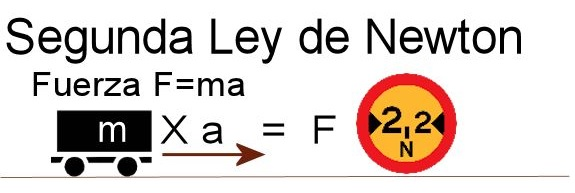
\includegraphics[scale=0.5]{images/segunda-ley-de-newton.jpg}
 % cinematica.png: 0x0 px, 300dpi, 0.00x0.00 cm, bb=
 \caption{Ilustración de la primera ley de Newton.}\label{ac}
\end{figure} 

Tambien conocida como \textbf{Ley de la Fuerza}, y dice:

\begin{tcolorbox}
"Si a un cuerpo de masa $m$ se le aplica una fuerza $\vec{F}$, ésta fuerza le produce una aceleración $a$."
\end{tcolorbox}

Esta aceleración es directamente proporcional a la Fuerza e inversamente proporcional a la masa, y esto se escribe así:

\begin{equation}
\vec{a} \propto \vec{F} \quad y \quad \vec{a} \propto \frac{1}{m}
\end{equation}

Uniendo estas dos proporcionalidades se obtiene que la fuerza es directamente proporcional a la masa y a la aceleración, y así 
queda como ecuación:

\begin{equation}
\vec{F} = m\vec{a} \quad [N]
\end{equation}
donde se ha tomado como constante de proporcionalidad la unidad, y las unidades de la fuerza es el Newton($N$), así mismo para el 
caso de varias fuerzas aplicadas en un cuerpo la ley se generaliza así:

\begin{equation}
\sum \vec{F} = m\vec{a}
\end{equation} 

\subsection{Tercera Ley de Newton}

\begin{figure}[ht]
 \centering
 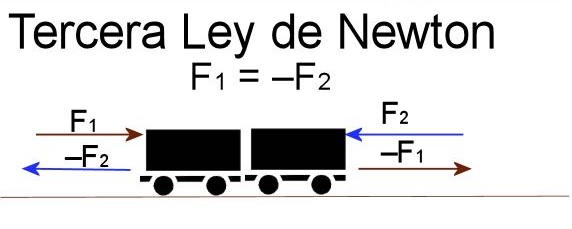
\includegraphics[scale=0.5]{images/tercera-ley-de-newton.jpg}
 % cinematica.png: 0x0 px, 300dpi, 0.00x0.00 cm, bb=
 \caption{Ilustración de la tercera ley de Newton.}\label{ac}
\end{figure}

A esta ley se la conoce como la \textbf{ley de la acción y reacción}, y dice:

\begin{tcolorbox}
''En el Universo las fuerzas nunca aparecen solas, sino en parejas donde una la acción y la otra la reacción, estás fuerzas son 
de igual tamaño pero de sentido contrario".
\end{tcolorbox}

\begin{equation}
\vec{F_{\text{acción}}} = -\vec{F_{\text{reacción}}}
\end{equation}

Es importante descatar que la fuerza de acción y reacción actuan sobre cuerpos diferentes no sobre el mismo.\\

Para abordar problemas de dinámica un poco complejos es importante definir bien algunos tipos de fuerza comunes:

\subsection{El Peso:}

El peso es la fuerza gravitatoria que actúa sobre un objeto que tiene masa ($g$). El peso es causado por la acción del campo 
gravitatorio local sobre la masa del cuerpo. Por ser una fuerza, el peso se representa como un vector, definido por su módulo, 
dirección y sentido, aplicado en el centro de gravedad del cuerpo y dirigido aproximadamente hacia el centro de la Tierra.\\

Clásicamente se calcula así:

\begin{equation}
\vec{P} = m\vec{g}
\end{equation}

\begin{figure}[ht]
 \centering
 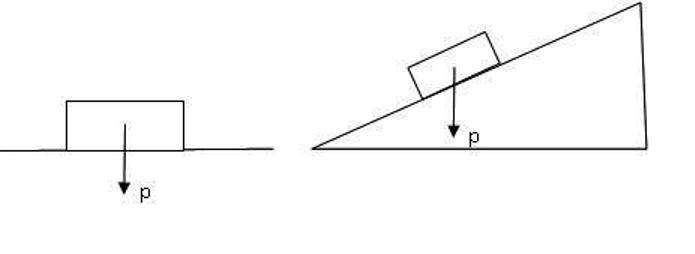
\includegraphics[scale=0.4]{images/peso.jpg}
 % cinematica.png: 0x0 px, 300dpi, 0.00x0.00 cm, bb=
 \caption{Ilustración de la dirección del peso en dos casos diferentes.}\label{ac}
\end{figure}

\subsection{La fuerza normal ($\vec{N}$):}

Es la fuerza que ejerce una superficie sobre un cuerpo apoyado sobre ella. Esta es de igual magnitud y dirección, pero de sentido 
contrario a la fuerza ejercida por el cuerpo sobre la superficie.La fuerza normal es una fuerza de contacto. Si dos superficies 
no están en contacto, no pueden ejercer fuerza normal una sobre la otra.\\

La fuerza normal es la fuerza que las superficies ejercen para prevenir que los objetos sólidos se atraviesen entre sí. Ésta 
fuerza siempre es perpendicular a la superficie de contacto.

\begin{figure}[ht]
 \centering
 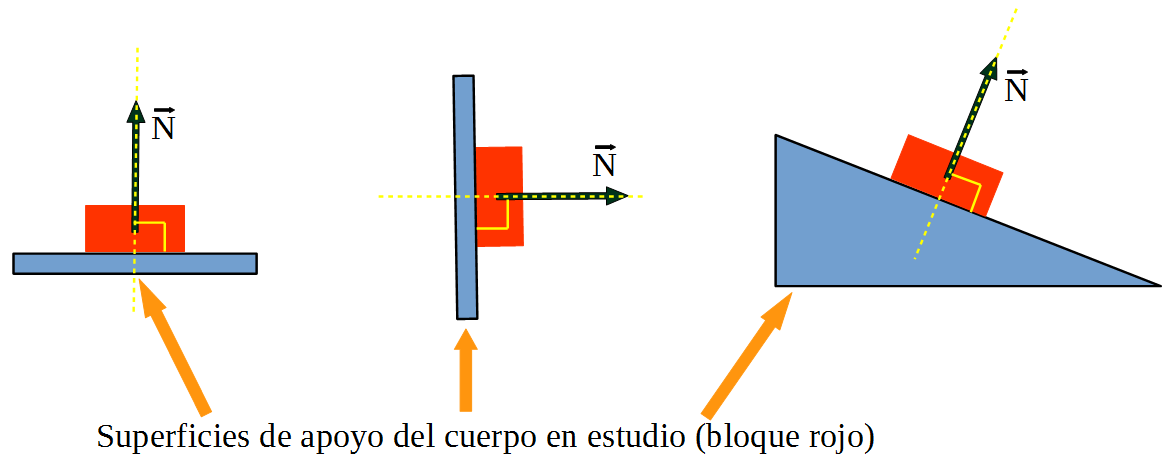
\includegraphics[scale=0.2]{images/fuerzanormal.png}
 % cinematica.png: 0x0 px, 300dpi, 0.00x0.00 cm, bb=
 \caption{Ilustración de la dirección de la fuerza normal en diferentes casos.}\label{ac}
\end{figure}

\subsection{Fuerzas de tensión ($\vec{T}$):}

Son aquellas fuerzas que se transmiten a tráves de cuerdas o hilos cuando se los tensiona.

\begin{figure}[ht]
 \centering
 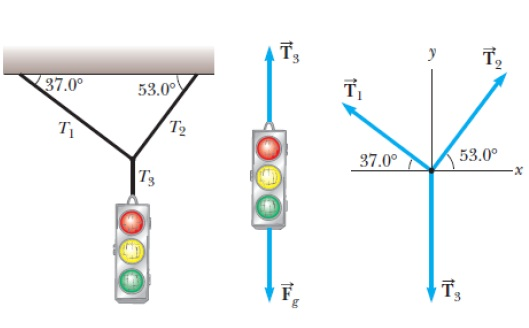
\includegraphics[scale=0.7]{images/tensiones.jpg}
 % cinematica.png: 0x0 px, 300dpi, 0.00x0.00 cm, bb=
 \caption{Ilustración de las tensiones sobre unas cuerdas que sostienen un semáforo.}\label{ac}
\end{figure}

\subsection{Fuerza de rozamiento:}

\begin{figure}[ht]
 \centering
 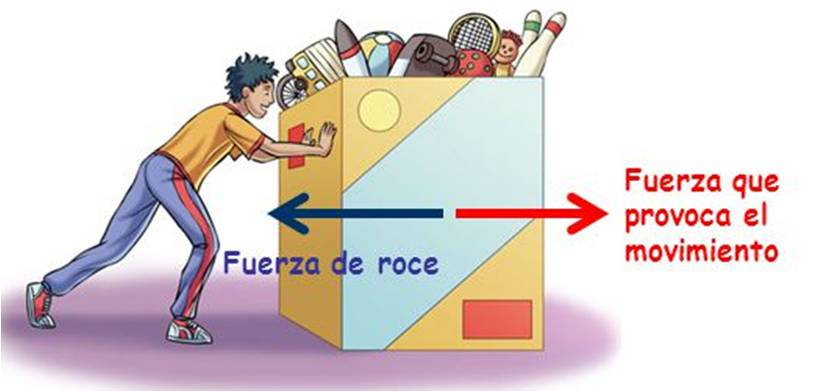
\includegraphics[scale=0.5]{images/fuerza-rozamiento.jpg}
 % cinematica.png: 0x0 px, 300dpi, 0.00x0.00 cm, bb=
 \caption{Ilustración de la fuerza de rozamiento.}\label{fr}
\end{figure}

Se trata de aquella fuerza que se origina cuando dos superficies en contacto se deslizan una sobre otra, debido a que las 
superficies, aún las que se consideran pulidas son extremadamente rugosas a escala microscópica. Es decir, esta fuerza es la que 
se opone al movimiento relativo entre ellas. Esta fuerza es de tipo disipativa, es decir, cuando esta se genera también se genera 
una pérdida de energía que se convierte en calor.\\

Esta fuerza de fricción se comporta de tal manera que cumple con los siguientes postulados básicos:\\

\textbf{a.} La resistencia al deslizamiento tangencial entre dos cuerpos es proporcional a la fuerza normal ejercida entre los 
mismos.
\textbf{b.} La resistencia al deslizamiento tangencial entre dos cuerpos es independiente de las dimensiones de contacto entre 
ambos.\\

La fuerza de fricción ($f_r$) en forma general se calcula de la siguiente manera:

\begin{equation}
f_r = \mu N
\end{equation}
  
donde $\mu$ es una constante adimensional\footnote{Se dice adimensional a aquellas cantidades que no poseen unidades de medida.} 
de llamada coeficiente de rozamiento que depende de la naturaleza de las superficies de rozamiento, que es además un número entre 
0 y 1, además, $N$ es la fuerza normal. Esta fuerza se opone al movimiento relativo al movimiento, por cuanto tendrá una 
dirección opuesta a este movimiento.  
    
\subsubsection{Tipos de Rozamiento:}

Existen dos tipos de rozamiento o fricción, la fricción estática ($f_{rs}$) y la fricción cinética ($f_{rk}$).\\ 
 
\textbf{Fuerza de fricción estática:}\\

Es la resistencia que se debe superar para poner en movimiento un cuerpo con respecto a otro que se encuentra en 
contacto. Se calcula así:

\begin{equation}
f_{rs} = \mu_e N
\end{equation}
donde $\mu_s$ es el coeficiente de rozamiento estatico.\\

\textbf{Fuerza de rozamiento cinética:}\\

Es la resistencia, de magnitud considerada constante, que se opone al movimiento pero una vez que este ya comenzó.

\begin{equation}
f_{rk} = \mu_k N
\end{equation}
donde $\mu_k$ es el coeficiente de rozamiento cinético.

\begin{figure}[ht]
 \centering
 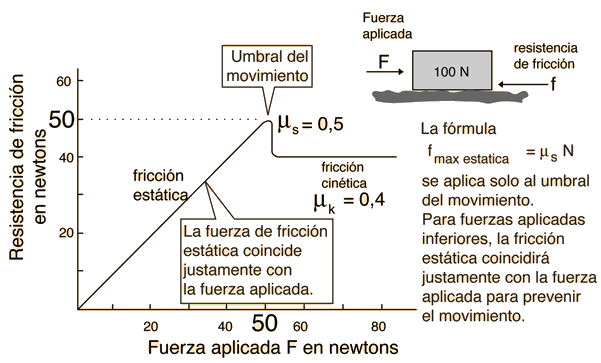
\includegraphics[scale=0.4]{images/fsta.png}
 % cinematica.png: 0x0 px, 300dpi, 0.00x0.00 cm, bb=
 \caption{Ilustración del comportamiento de la fuerza de fricción.}\label{frb}
\end{figure}

En la figura \ref{frb} se puede apreciar como actua el rozamiento cuando se mueve un cuerpo desde el reposo, primero se genera 
fuerza de rozamiento estática ($f_{rs}$) que se va incrementando desde cero hasta un valor máximo donde se supone que el cuerpo 
que se quiere mover comienza a moverse, luego esta fuerza de rozamiento disminuye en valor teniéndose de hecho a lo que se llama 
fuerza de rozamiento cinético ($f_{rk}$).

\section{Diagrama de cuerpo libre:}

Para la resolución de sistemas dinámicas usualmente se usa una técnica llamada el diagrama de cuerpo libre que consiste en un 
boceto de un objeto de interés despojado de todos los objetos que lo rodean y mostrando todas las fuerzas que actúan sobre el 
cuerpo.\\

Consiste en colocar la partícula en el origen de un plano de coordenadas, y representar a las fuerzas que actúan sobre ella por 
medio de los vectores correspondientes, todos concurrentes en el origen. La mayor aplicación de los DCL es visualizar mejor el 
sistema de fuerzas que actúan sobre un cuerpo; además, se identifican mejor las fuerzas pares, como la de acción - reacción y las 
componentes de las fuerzas.\\

Si en un sistema existen dos o más cuerpos de interés, éstos se deben separar y cada uno tiene un DCL propio con sus respectivas 
fuerzas actuando.

\begin{figure}[H]
 \centering
 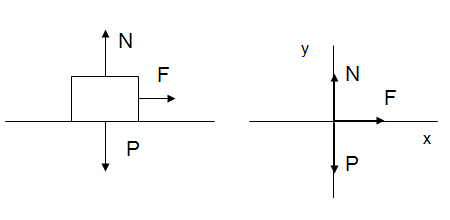
\includegraphics[scale=0.6]{images/cuerpo-libre.png}
 % cinematica.png: 0x0 px, 300dpi, 0.00x0.00 cm, bb=
 \caption{Ilustración de un ejemplo de diagrama de cuerpo libre.}\label{frb}
\end{figure}

\subsection{Problemas de Dinámica}

\begin{enumerate}
 \item Una fuerza neta de 7.5 kN dirigida hacia el oeste actúa sobre un auto de carreras de 1208 kg. ¿A qué velocidad acelerará 
el auto?

\item  ¿Cuál es la masa de un cuerpo, si
 al aplicarle una fuerza de 200 N le produce una aceleración de $40 m/s^2$?

\item  ¿Cuánto tiempo deberá actuar
 una fuerza de 250 N sobre un cuerpo de 12,5 kg para lograr detenerlo si va a una velocidad 
de
 720 km/h?

 \item Un automóvil, con una masa de 1485 kg viaja hacia el sur a 116 km/h, disminuye su velocidad en 10.25 segundos. ¿Cuál es la 
magnitud y la dirección de la fuerza neta que actuó en el camión?

\item Un ascensor pesa 400 Kg. ¿Qué fuerza debe ejercer el cable hacia arriba para que suba con una aceleración de $5 m/s^2$?.

\item Una pelota de fútbol de 550 g de masa adquiere una
 velocidad de 70 m/s mediante un puntapié de 0,2 s de duración, ¿qué 
fuerza recibió la pelota?

\item Una locomotora de 8000 kg de masa tira de un tren de 40000 kg a lo largo de una vía nivelada y lo mueve con una aceleración 
de $1,2 m/s^2$. ¿Con qué aceleración tiraría a un tren de 16000 kg?

\item Resover el problema anterior si la vía descrita tiene un ángulo de $12^\circ$ con respecto a la horizontal.

\item  Una grúa eleva una masa m = 800 kg
 mediante un cable que soporta una tensión de 12000 N. ¿Cuál es la máxima aceleración 
con que
 se puede elevar?

\item Un vehículo de 150 kg de masa se mueve en línea recta a 70 km/h. ¿Qué fuerza debe aplicarse en forma constante para que 
reduzca su velocidad a 20 km/h durante los siguientes 10 segundos de aplicada la fuerza?

\item Calcula la fuerza que habrá que realizar para frenar, hasta detener en 10 segundos un trineo que se mueve a 50 km/h.

\item ¿Cómo cambia la el valor de la aceleración que adquiere un cuerpo si se duplica su masa y se reduce a la mitad el módulo de 
la fuerza aplicada sobre el mismo?.

\item Un vehículo de 800 kg se mueve en un tramo recto y horizontal de autovı́a a 72 km/h. Si por una averı́a deja de funcionar 
el motor y se detiene a los 100 m, calcula la fuerza de rozamiento.

\item ¿Cuál es la masa de un cuerpo, si al aplicarle una fuerza de 420 N de produce una aceleración de $8.4 m/s^2$ ?

\item ¿Cuánto tiempo deberá actuar una fuerza de 80 N sobre un cuerpo de masa de 12.5 kg para lograr detenerlo si va a una 
velocidad de 720 km/h?

\item ¿Cuál es la fuerza necesaria para que un móvil de 1500 kg, partiendo de reposo adquiera una rapidez de $2 m/s^2$ en 12 s?

\item Calcular la masa de un cuerpo, que estando de reposo se le aplica una fuerza de 150 N durante 30 s, permitiéndole recorrer 
10 m. ¿Qué rapidez tendrá al cabo de ese tiempo?

\item  Una auto se mueve a una 
velocidad de 36 km/h, y de pronto debe frenar hasta detenerse antes de cruzar con un semáforo en 
rojo que se ubica a 0,1 km. Determine la fuerza de frenado si el auto tiene una masa de 500 kg.

\item  Si una fuerza se aplica a un 
cuerpo de masa $m$ éste adquiere una aceleración. Si la misma fuerza se aplica a un cuerpo 
de 
masa $2m$, ¿Cuál sería su aceleración?

\item Calcular la magnitud de la aceleración que produce una fuerza cuya magnitud es de 50 N a un cuerpo cuya masa es de 13,000 
gramos.

\item Determinar la magnitud de la fuerza que recibe un cuerpo de 45 kg, la cual le produce una aceleración cuya magnitud es de 
$7 
m/s^2$.

\item Una bala de 0,25 g de masa sale de un cañón de un rifle con una velocidad de 350m/s. ¿Cual es la fuerza promedio que se 
ejerce sobre la bala mientras se desplaza por el cañón de 0.8 m de longitud del rifle?

\item Un carrito de juguete de 3 kg parte del reposo y se mueve una distancia de 4 m en 2 s bajo la acción de una fuerza 
constante 
única.Encuentre la magnitud de la fuerza. 

\item ¿Cuál es la fuerza necesaria para que un móvil de 1700 Kg, partiendo de reposo adquiera una rapidez de $2 m/s^2$ en 12.4 s?

\item Un protón tiene una masa de $1,7 \times 10^{−27} kg$ y se mueve con una velocidad de $2 \times 10^8 m/s$. ¿Qué fuerza será 
necesaria para reducir su velocidad a $10^8 m/s$ en 0.0001 s?

\item Calcular la velocidad final con la que un bloque de masa 10 kg llega a la parte inferior de un plano inclinado de 20 cm 
de largo y 15 cm de alto. Considérese que no hay fuerzas de rozamiento y que la el valor de la aceleración de la gravedad
igual a $10 m/s^2$.

\item Dos bloques de masas $m_1 = 20 kg$ y $m_2 = 8 kg$, están unidos mediante una cuerda homogénea inextensible que pesa 2 kg. Se
aplica al conjunto una fuerza vertical hacia arriba de 560 N. Calcular: a) La aceleración del conjunto; b) Las fuerzas que actúan 
en los extremos de la cuerda.

\item Un astronauta percibe que se aleja lentamente de la estación espacial y la cuerda que lo conecta está rota. En sus manos 
tiene un equipo de 5 kg. ¿Qué podría hacer el astronauta de forma rápida para intentar volver a la estación espacial?     

\end{enumerate}


\chapter{Trabajo y Energía}

\textit{``El movimiento es un modo de ser que resulta necesariamente de la materia; ésta se mueve por su propia energía; sus 
movimientos se deben a las fuerzas que le son inherentes.''}\textbf{Barón de Holbach}\vspace{1.0 cm}

El concepto de energía (\textbf{E}) es uno de los más utilizados y destacados en esta ciencia. En este Universo la energía juega 
un papel muy importante, es aquella encargada del movimiento de los cuerpos y que los procesos naturales sean posibles.

\begin{tcolorbox}
La energía es la capacidad que poseen los cuerpos para poder efectuar un trabajo (movimiento) o de lograr alguna transformación.  
\end{tcolorbox}

Según la forma o el sistema físico en que se manifiesta, se consideran diferentes formas de energía: térmica, mecánica, 
eléctrica, 
química, electromagnética, nuclear, luminosa, etc. En cuanto a su unidad de medida es el "JOULE" ó "JULIO", que se denota 
simplemente como \textbf{J}.\\

Aunque la energía puede cambiar de forma en los procesos de conversión energética, la cantidad de energía se mantiene constante 
conforme con el \textbf{principio de conservación de la energía} que establece:

\begin{tcolorbox}
``La energía no se crea ni se destruye, sólo se transforma''. 
\end{tcolorbox}

Por consiguiente, la energía total de un sistema aislado se mantiene constante y en el universo no puede existir creación o 
desaparición de energía, sino transferencia de un sistema a otro o transformación de energía de una forma a otra, es en otras 
palabras, la energía es una invariante física. Así en un sistema aislado se tendrá que la energía total de cuyo sistema es el 
mismo, es decir:

\begin{equation}
E_{inicio} = E_{final}
\end{equation}

En este momento nos referiremos específicamente a la energía mecánica ($E_m$) la cual es aquella relacionada con el fenómeno del 
movimiento, y así está energía se la puede visualizar como la suma de la energía cinética ($E_c$), la energía potencial 
gravitatoria ($E_p$) y la energía potencial elástica ($E_k$), así inicialmente:

\begin{equation}
E_m = E_c + E_p + E_k \quad [J]
\end{equation} 

\section{Energía cinética:}

Esta energía es la que tiene un cuerpo movimiento por el simple hecho de que tiene una velocidad diferente de cero. Por tanto la 
energía que tiene un cuerpo de masa $m$ cuya velocidad $v$ es:

\begin{equation}
E_c = \frac{1}{2}mv^2
\end{equation}

\section{Energía potencial gravitatoria:}

Está energía está asociada a la posición que tienen los cuerpos, y no a su movimiento. Se define como aquella que poseen los 
cuerpos por el hecho de encontrarse en una determinada posición en un campo de fuerzas.\\

Un concepto más acertado es el siguiente:

\begin{tcolorbox}
La energía potencial gravitatoria. de una masa en un punto del espacio es el trabajo que realiza en un campo gravitatorio para 
trasladar la masa desde dicho punto hasta el infinito. 
\end{tcolorbox}

Es decir, está energía es la que posee un cuerpo por el hecho de encontrarse bajo la acción de la gravedad. Su valor, para el 
caso 
de alturas pequeñas sobre la superficie terrestre, viene dado por:

\begin{equation}
E_p = mgh
\end{equation}

donde la $h$ es la altura del cuerpo con respecto al suelo.

\section{Energía Potencial Elástica:}

Esta energía es la que se almacena o se libera cuando un resorte es comprimido o estirado, esta energía depende del material del 
resorte como también de la variacción de su longitud al ser manipulado.\\

Todo resorte tiene una constante elástica $k$ llamada constante de elásticidad del resorte y está relacionado con la energía 
potencial elástica ($E_k$) como:

\begin{equation}
E_k = \frac{1}{2}k\Delta x^2
\end{equation}

donde $\Delta x$ es la longitud comprimida o alargada el resorte por una fuerza. Un concepto más acertado de está energía es el 
trabajo realizado por una fuerza al comprimir o alargar un resorte.

Se ha mencionado el término de trabajo, por lo cual es pertinente conocer el significado físico de ese término.

\section{Trabajo mecánico:}

El trabajo mecánico es la capacidad de una fuerza para desplazar un cuerpo una cierta distancia. Es decir, es esa energía 
necesaria para poder mover a ese cuerpo una distancia mediante una fuerza.\\

\begin{figure}[ht]
 \centering
 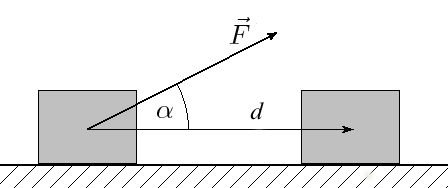
\includegraphics[scale=0.5]{images/trabajo.png}
 % cinematica.png: 0x0 px, 300dpi, 0.00x0.00 cm, bb=
 \caption{Ilustración del trabajo mecánico.}\label{tmec}
\end{figure}

El trabajo es una magnitud física escalar que se representa con la letra $W$ y se expresa en unidades de energía (\textbf{J}) en 
el Sistema Internacional de Unidades. Para el cálculo del trabajo sólo se tiene en cuenta la componente de la fuerza que actúa en 
la dirección de desplazamiento del cuerpo, por lo que el trabajo es una magnitud escalar. De este modo el trabajo se computa así:

\begin{equation}
W = \vec{F}\cdot\vec{\Delta r}\quad [J]
\end{equation}

donde se observa que el trabajo mecánico es el producto escalar entre la fuerza $\vec{F}$ y el desplazamiento $\Delta \vec{r}$ 
que 
realiza el cuerpo bajo la influencia de $\vec{F}$.\\

El trabajo mecánico puede tener dos signos: uno positivo y otro negativo. El signo positivo es cuando la fuerza aplicada va en el 
mismo sentido del movimiento, pero es negativo cuando va en contra del movimiento, ya que el trabajo mecánico es:

\begin{equation}
W = F\Delta r cos(\theta)
\end{equation}
 
siendo el $\theta$ el ángulo entre la fuerza $\vec{F}$ y el desplazamiento $\Delta \vec{r}$. También, existe el caso cuando el 
trabajo es nulo que correspondería cuando la fuerza y el desplazamiento son perpendiculares entre sí.
  
\section{Potencia:}  

La potencia se puede entender como la rapidez con la que se efectúa trabajo y se define como el trabajo realizado por unidad de 
tiempo. La potencia mecánica se simboliza con la letra P

\begin{equation}
P = \frac{W}{\Delta t}\quad [W]
\end{equation}

También la potencia la podemos expresar en término de la velocidad, para cuando la fuerza es constante

\begin{equation}
P = Fv
\end{equation}

Las unidad de medida para la potencia en el S.I son el Watts ($W$), el cual se define como $Joule/s$.

\section{Problemas de trabajo y energía}

\begin{enumerate}

\item Un hombre sube por las escaleras de un edificio llevando a cuestas una lavadora que pesa 500 N, y cuando llega al octavo 
piso, se había dado cuenta que se ha equivocado de edificio, y regresa a la planta baja. Si el octavo piso esta a 20 metros de 
altura, ¿cuál fue el trabajo realizado por el hombre durante su recorrido?

\item Se suelta un bloque de masa de 10 kg desde lo alto de un plano inclinado que forma un ángulo de $30^\circ$ con la
horizontal y de longitud 50 cm. El bloque choca contra un resorte horizontal ideal y lo deforma 10 cm en la parte baja del plano 
inclinado. Conociendo que el coeficiente de rozamiento entre el plano inclinado y el bloque es 0.3; determine la constante 
elástica del resorte.

\item Un pedazo de plastilina, de 40 g de masa, se mueve con velocidad de 100 m/s y choca, quedando incrustada, en un bloque de 
madera de 1 kg de masa que está en reposo. El bloque está unido a un muelle que se contrae 20 cm. Si no hay rozamiento entre 
el suelo y el bloque, determina el periodo de oscilación del movimiento vibratorio generado.

\item Una maceta cae de un balcón a una velocidad de 9,81m/s adquiriendo una energía cinética de 324J, ¿cuál es su masa?  

\item Una persona transporta sobre sus hombros un bulto de 25 kg con el que recorre 20 m. Determina el trabajo realizado para 
soportarlo. 

\item Un automóvil de 1.500 kg lleva una velocidad de 120 km/h por una carretera horizontal. En un determinado momento ve un 
obstáculo y frena hasta pararse. Calcula el trabajo realizado.

\item Un automóvil de 1.000 kg tarda 8 segundos en alcanzar la velocidad de 72 km/h.¿Qué potencia desarrolla el motor sabiendo 
que 
la fuerza de rozamiento es equivalente a la décima parte del peso? 

\item Se tiene un plano inclinado cuya longitud es 15 m y cuya base es 9 m. ¿Con qué velocidad y con qué energía cinética  
llegará 
a su extremo inferior un cuerpo de 60 Kg que partió del extremo superior con una velocidad de 2 m/s? 

\item  Si la masa de un cuerpo se duplica y su velocidad se reduce a la cuarta parte, ¿cómo cambia su cantidad de energía 
cinética?

\item  Una pelota de fútbol de 550 g de masa adquiere una velocidad de 70 m/s mediante un puntapié de 0,2 s de duración, ¿cuál 
es el trabajo mecánico realizado por la fuerza ? 

\item  Sobre un cuerpo de 10 kg de masa actúa una fuerza de 100N que forma un ángulo de 30º con la horizontal que hace que se 
desplace 5 m. Si el coeficiente de rozamiento entre el cuerpo y el suelo es 0,2, calcula el trabajo realizado por la normal. 

\item Calcule la potencia realizado por un motor de un ascensor de 300 kg que se eleva a una velocidad 0.5 m/s.

\item Un paquete es lanzado por un plano inclinado $20^\circ$ con la horizontal con una velocidad de 8m/s en un punto A del 
plano. Llega a un punto B situado 7 m más arriba de A y se detiene. ¿Cuál es el coeficiente de fricción entre el paquete y el
plano inclinado?

\item Un cuerpo de 1,5 kg de masa cae desde 60 m. Determinar la energía potencial y cinética a 15 metros antes de topar el piso.

\item  Un motor eléctrico realiza trabajo sobre un compresor a un ritmo de 1.5 KW. ¿Cuánto trabajo ha realizado en un mes si el 
compresor funciona ininterrumpidamente?

\item Una fuerza de 150 N paralela a un plano inclinado de ángulo $30^\circ$ actúa sobre un cuerpo de masa 10 Kg. Si el cuerpo 
asciende 5 m por el plano inclinado y μ= 0,2. Calcular la energía perdida como calor.

\item  Un cuerpo 4 kg cae desde 2,3 m de altura sobre un resorte cuya constante es 200 N/m. Calcular la velocidad del cuerpo 
cuando el resorte se ha comprimido 2.5 cm.

\item Se deja caer sobre un muelle en posición vertical una masa de 0.5 kg desde 1 m de altura. El muelle tiene una longitud de 
0.5 m y una constante de 100 N/m. Calcular la longitud h del muelle cuando está comprimido al máximo.

\begin{figure}[h]
 \centering
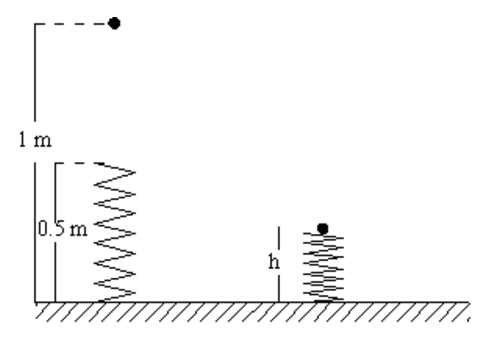
\includegraphics[width=4.0cm,height=3.0cm]{images/energia.eps}
\end{figure}

\item Desde la parte más baja de un plano inclinado, sube un bloque hasta detenerse en la parte más alta del mismo plano. Si la 
energııa mecánica total del bloque en la parte inferior y la superior es de 100J y 70 J, respectivamente, determine el 
coeficiente de rozamiento entre el bloque y el plano.

\item Se lanza una pelota desde 2m de altura. En el segundo rebote la altura que alcanza es 0.35 m. ¿Qué porcentaje de energía 
pierde cada vez que rebota?

\item Se suelta un bloque de masa de 10 kg desde lo alto de un plano inclinado que forma un ángulo de $30^\circ$ con la 
horizontal y de longitud 50 cm. El bloque choca contra un resorte horizontal ideal y lo deforma 10 cm en la parte baja del plano 
inclinado. Conociendo que el coeficiente de rozamiento entre el plano inclinado y el bloque es 0.3; determine la constante 
elástica del resorte.

\item  Un paquete es lanzado por un plano inclinado $20^\circ$ con la horizontal con una velocidad de 8m/s en un punto A del 
plano. Llega a un punto B situado 7 m más arriba de A y se detiene. ¿Cuál es el coeficiente de fricción entre el paquete y el 
plano inclinado?

\item El quarterback de un equipo de fútbol americano lanza el balón (435 gramos de masa) con una velocidad de 18 m/s y ángulo de 
$50^\circ$ respecto a la dirección horizontal. Debido a la fricción del aire, el balón cae al suelo 0,5 metros antes de lo que 
habría alcanzado en ausencia de la fricción. Con base en lo mencionado anteriormente y suponiendo una fricción constante en la 
dirección de horizontal, determine: a) La aceleración que imparte la fricción del aire al balón, b) el trabajo realizado por 
dicha fricción sobre el balón, y c) la energía cinética que el balón pierde debido a esta fricción. 


\end{enumerate}


\chapter*{Bibliografía:}

\begin{enumerate}
\item Kuhn, Thomas S., "The Function of Measurement in Modern Physical Science", ISIS 52(2), 161?193, 1961.
 
\item Molina M.J.T.- El Método Científico Global.
 
\item René Descartes. Discurso del método. segundo título o indicación al título principal Discours de la methode. Pour bien 
conduire la raison \& chercher.
 
\item Rozenberg, I. M. (2002). O sistema internacional de unidades-SI. Instituto Mauá de Tecnologia.
 
\item Alonso M., O. Rojo, FÍSICA: Mecánica y Termodinámica, Adisson Wesley, 1979.

\item Panchi Nuñez C., Física Vectorial Elemental, Vol. 1, 8va Ed. Quito,1999.

\item P. Vallejo, J. Zambrano, Física Vectorial, Vol. 1, Séptima Edición, 2019.

\item Profesores del Curso Propedéutico de la Escuela Politécnica Nacional, FÍSICA PARA PREPOLITÉCNICO, PrepoFis Pub, Quito, 2011.  

\end{enumerate}



\end{document}
